\documentclass[11pt]{article}
\usepackage{debulletin,times,epsfig,subfigure,wrapfig,algorithmic,color,boxedminipage,graphicx,url}
% this is the template for an issue of the Data Engineering Bulletin

% all packages used by any paper must be listed here
%\usepackage{hyperref}
%\usepackage{authblk}
%\setlength{\affilsep}{0em}
%\usepackage{inputenc}
%\usepackage{debulletin}
%\usepackage{times}
%\usepackage{graphicx}
%\usepackage{array}
%\usepackage{wrapfig}
%\usepackage[table]{xcolor}
%\usepackage{tcolorbox}
%\usepackage{amssymb}
%%\usepackage[labelfont=bf,labelsep=space,list=true]{subcaption}
%\usepackage{url}
%\usepackage{mathtools, bm}
%\usepackage{float}
%\usepackage{multirow}
%\usepackage{multicol}
%\usepackage{algorithm}
%\usepackage{subfig}
%\usepackage{algpseudocode}
%\setlength{\intextsep}{10pt plus 2pt minus 2pt}
%\hyphenation{finally}

\usepackage{amsmath, amssymb, amsfonts}

\usepackage{hyperref}
\usepackage{enumitem}
\usepackage{xspace} 
%\usepackage{xcolor}
\usepackage{tikz}
\usepackage[T1]{fontenc}
\usepackage{beramono}
\usepackage{listings}
\usepackage{xcolor}



\usepackage{wrapfig}

\usepackage{graphics}
\usepackage{pifont}
%\usepackage{subcaption} % for subtable
%\usepackage{threeparttable} % for tablenotes




\usepackage[numbers]{natbib}
% \documentclass{article}
% Recommended, but optional, packages for figures and better typesetting:
\usepackage{microtype}
\usepackage{graphicx}
% \usepackage{subfigure}
\usepackage{booktabs} % for professional tables
%\usepackage[table,dvipsnames]{xcolor}
\usepackage{epsfig}
\usepackage{pgfplotstable}
\usepackage{pgfplots}
\usepgfplotslibrary{groupplots}
\usepackage{bbm}
\usepackage{booktabs}
\usepackage{verbatim}
\usepackage[T1]{fontenc}
\usepackage{caption}
\usepackage{siunitx}
\usepackage{xspace}
%\usepackage[colorinlistoftodos,textsize=footnotesize]{todonotes}
%\usepackage[utf8]{inputenc}
\usepackage[autostyle, english=american]{csquotes}
\usepackage{breakurl}




\begin{document}


% please enter real date, vol no, issue no
\bulletindate{December 2020}
\bulletinvolume{43}
\bulletinnumber{4}
\bulletinyear{2020}

% these are files that I have- but your part of the issue can be done without
% them
\IEEElogo{cs.pdf}
\insidefrontcover{incvA19.pdf}
%\insidebackcover[ICDE Conference]{./calls/icde-new-a.ps}

\begin{bulletin}

% the above samples assume the issue is generated from a directory structure of the following sort
% major directory name is month and year of issue
% there are sub-directorys for
% letters: directory name is "letters"
% technical articles: a directory per paper, named for an "author"
% news articles: directory name is "news"
% calls: directory name is "calls

%
%  Editor letters section.  Use the lettersection environment.
%  Each letter is contained in a letter environment, where the two required
%  options to \begin{letter} are the author and the address of the author.
%

\begin{lettersection}

% there will be other letters- and a blank page will appear in your document
% but the special issue part will be fine

\begin{letter}{Letter from the Editor-in-Chief}
{Haixun Wang}{WeWork Corporation}
\documentclass[11pt]{article} 

\usepackage{deauthor,times,graphicx}
%\usepackage{url}
\usepackage{hyperref}

\begin{document}
Around the time we published our last issue in March, the nation went
into a lockdown. Life in the last 3 months has been unprecedented in
many ways. As governments around the world scrambled to fight
coronavirus, people in the scientific community, especially those on
the frontline -- doctors, healthcare professionals, medical staff and
researchers -- made heroic efforts and sacrifices to curb the pandemic
and save lives. The data management and data science communities also
sprang to action immediately. Globally, it is the first time that data
driven approaches are being used at such a large scale toward solving
a common problem. Under this backdrop, in this special issue of the
Data Engineering Bulletin edited by Joseph Gonzalez, we feature 8
papers on the topic of {\it digital contact tracing}, a technique that
may prove crucial in the fight against Covid-19.

This issue also features two opinion pieces. Divyakant Agrawal and Amr
El Abbadi's wake-up call on managing data in an untrusted environment
takes us to the fascinating world of cryptocurrencies and
blockchains. It shows what the database community, which was
responsible for creating and perfecting transaction management and
distributed systems, can learn from the blockchain approach when it
comes to handling untrusted behaviours from the underlying
infrastructure. The second opinion piece, written by Jeffrey
D. Ullman, addresses a question on the mind of every data management
person: What is our role in the machine learning and AI revolution?
Have we missed the boat again and become irrelevant? Ullman's
perspective, illustrated by his remake of the well known Conway Venn
Diagram that illustrates the relationship between computer science,
mathematics \& statistics, and domain knowledge is incisive,
thought-provoking, and entertaining at the same time.
\end{document}


\end{letter}
%
\newpage
%
%% your introductory letter goes here
%
\begin{letter}{Letter from the Special Issue Editor}
{James Foulds and Shimei Pan}{University of Maryland, Baltimore County}
\documentclass[11pt]{article} 

\usepackage{deauthor,times,graphicx}
%\usepackage{url}

\begin{document}

Software applications that learn from data using machine learning (ML) are being deployed in increasing numbers in the real world. Designing and operating such applications introduces novel challenges, which are very different from the challenges encountered in traditional data processing scenarios. ML applications in the real world exhibit a much higher complexity than ``text book'' ML scenarios (e.g., training a classifier on a pre-existing dataset). They do not only have to learn a model, but must define and execute a whole ML pipeline, which includes data preprocessing operations such as data cleaning, standardisation and feature extraction in addition to learning the model, as well as methods for hyperparameter selection and model evaluation. Such ML pipelines are typically deployed in systems for end-to-end machine learning, which require the integration and validation of raw input data from various input sources, as well as infrastructure for deploying and serving the trained models. The system must also manage the lifecycle of data and models in such scenarios, as new (and potentially changing) input data has to be continuously processed, and the corresponding ML models have to be retrained and managed accordingly. The majority of these challenges have only recently begun to attract the attention of the data management community. 
%
A major obstacle is that the behavior of ML-based systems heavily depends on the consumed input data, which can rapidly change, for example due to changed user behavior or due to errors in external sources that produce the inputs. This area represents a gap between the data management and ML communities: research in ML mostly focuses on learning algorithms, and research in data management is mostly concerned with data processing and integration. In this issue, we focus on this gap in data validation for machine learning, and provide perspectives from both the academic and industrial research communities to learn about the state of the art, open problems and to uncover interesting research directions for the future.

The first paper presents \textit{A Data Quality-Driven View of MLOps} and demonstrates how different aspects of data quality propagate through various stages of machine learning development. It connects data quality to the downstream machine learning process, an approach that is also taken by our second paper, which argues that we should move \textit{From Cleaning before ML to Cleaning for ML}. The authors propose an end-to-end approach to take the entire application's semantics and user goals into account when cleaning data, instead of performing the cleaning operations in an isolated manner beforehand.

The next two papers on \textit{Validating Data and Models in Continuous ML pipelines} and \textit{Automated Data Validation in Machine Learning Systems} from Google and Amazon provide us with an industry perspective on the area in the focus of this issue. The first paper describes tools developed at Google for the analysis and validation of two of the most important types of artifacts: Datasets and Models. These tools (which are part of the Tensorflow Extended Platform) are currently deployed in production at Google and other large organizations, and are heavily inspired by well-known principles of data-management systems. The second paper from Amazon reviews some of the solutions developed to validate data at the various stages of a data pipeline in modern ML applications, discusses to what extent these solutions are being used in practice, and outlines research directions for the automation of data validation.

The subsequent paper on \textit{Enhancing the Interactivity of Dataframe Queries by Leveraging Think Time} focuses on the highly exploratory and iterative nature of data validation in the early stages of an ML application, where data scientists start with a limited understanding of the data content and quality, and perform data validation through incremental trial-and-error. The final paper of this issue on \textit{Responsible AI Challenges in End-to-end Machine Learning} completes the view on data validation for machine learning by connecting it with pressing issues from the area of responsible data management.\\ 

Working on this issue has been a privilege for me, and I would like to thank the authors for their  contributions.


\end{document}


\end{letter}

\end{lettersection}

% put the name of your special issue below

%\begin{opinionsection}
%\begin{opinion}{Entities with Quantities}
%{Gerhard Weikum}{Max Planck Institute for Informatics}
%\documentclass[11pt]{article} 

\usepackage{deauthor,times,graphicx}
%\usepackage{url}
\usepackage{hyperref}

\begin{document}
Around the time we published our last issue in March, the nation went
into a lockdown. Life in the last 3 months has been unprecedented in
many ways. As governments around the world scrambled to fight
coronavirus, people in the scientific community, especially those on
the frontline -- doctors, healthcare professionals, medical staff and
researchers -- made heroic efforts and sacrifices to curb the pandemic
and save lives. The data management and data science communities also
sprang to action immediately. Globally, it is the first time that data
driven approaches are being used at such a large scale toward solving
a common problem. Under this backdrop, in this special issue of the
Data Engineering Bulletin edited by Joseph Gonzalez, we feature 8
papers on the topic of {\it digital contact tracing}, a technique that
may prove crucial in the fight against Covid-19.

This issue also features two opinion pieces. Divyakant Agrawal and Amr
El Abbadi's wake-up call on managing data in an untrusted environment
takes us to the fascinating world of cryptocurrencies and
blockchains. It shows what the database community, which was
responsible for creating and perfecting transaction management and
distributed systems, can learn from the blockchain approach when it
comes to handling untrusted behaviours from the underlying
infrastructure. The second opinion piece, written by Jeffrey
D. Ullman, addresses a question on the mind of every data management
person: What is our role in the machine learning and AI revolution?
Have we missed the boat again and become irrelevant? Ullman's
perspective, illustrated by his remake of the well known Conway Venn
Diagram that illustrates the relationship between computer science,
mathematics \& statistics, and domain knowledge is incisive,
thought-provoking, and entertaining at the same time.
\end{document}


%\end{opinion}
%\end{opinionsection}

\begin{articlesection}{Interdisciplinary Perspectives on Fairness and Artificial Intelligence Systems}
%
%  Contributed articles section.  Use the articlesection environment.
%  Each article is contained in an article environment, where the two required
%  options to \begin{article} are the title and author of the article
%

%\makeatletter
%\renewcommand{\AB@affillist}{}
%\renewcommand{\AB@authlist}{}
%\setcounter{authors}{0}
%\makeatother

\begin{article}
{Transforming the Culture: Internet Research at the Crossroads}
{Safiya Umoja Noble and Sarah T. Roberts}
\graphicspath{{submissions/NobleRoberts_final/}}
%\documentclass[11pt,dvipdfm]{article}
\documentclass[11pt]{article}
\usepackage{deauthor,times,graphicx,hyperref} 

\usepackage{amsmath, amssymb, amsfonts}  

%\usepackage{algorithmic}
%\usepackage{graphicx}
%\usepackage{textcomp}
%\usepackage{xcolor}
\def\BibTeX{{\rm B\kern-.05em{\sc i\kern-.025em b}\kern-.08em
    T\kern-.1667em\lower.7ex\hbox{E}\kern-.125emX}}

%\usepackage{graphicx}
%\usepackage{subfigure}
%\usepackage{hyperref}
%\usepackage{enumitem}
%\usepackage{multirow}
%\usepackage{dsfont}
%\usepackage{algorithm2e}
%\usepackage[table,xcdraw]{xcolor}
%\usepackage{booktabs}

%\usepackage{tikz}
%\usetikzlibrary{bayesnet}

\usepackage{breakcites} %Fixes citations exceeding the margin!!

% \newtheorem{example}{Example} 
% \newtheorem{theorem}{Theorem}
% \newtheorem{lemma}[theorem]{Lemma} 
% \newtheorem{proposition}[theorem]{Proposition} 
 %\newtheorem{remark}[theorem]{Remark}
% \newtheorem{corollary}[theorem]{Corollary}
% \newtheorem{definition}[theorem]{Definition}
% \newtheorem{conjecture}[theorem]{Conjecture}
% \newtheorem{axiom}[theorem]{Axiom}
%%%
%\newtheorem{dfn}[theorem]{Definition}

%\usepackage{todonotes}
%\newcommand{\jf}[1]{{\bf \color{orange}{jf: #1}}}
%\newcommand{\shimei}[1]{{\bf \color{blue}{shimei: #1}}}
\setcounter{topnumber}{2}
\setcounter{bottomnumber}{2}
\setcounter{totalnumber}{4}
\renewcommand{\topfraction}{0.85}
\renewcommand{\bottomfraction}{0.85}
\renewcommand{\textfraction}{0.15}
\renewcommand{\floatpagefraction}{0.7}

% Definitions of handy macros can go here

\newcommand{\dataset}{{\cal D}}
\newcommand{\fracpartial}[2]{\frac{\partial #1}{\partial  #2}}

\begin{document}
\title{Transforming the Culture: Internet Research at the Crossroads}
\author{Safiya Umoja Noble \\
University of California, Los Angeles \\
snoble@g.ucla.edu
\and
Sarah T. Roberts\\ 
University of California, Los Angeles \\ 
sarah.roberts@ucla.edu}


\maketitle
\begin{abstract}
The topic of justice, fairness, bias, labor and their relation the products and practices of technology and internet companies has been a subject of our concern for nearly a decade. We see these challenges--from the organizing logics of the technology sector with respect to algorithmic discrimination, to labor practices in commercial content moderation, as key pathways into better understanding the creation and maintenance of problems made by the technology sector that cannot be solved with techno-solutionism. While our work has been closely aligned to research and advocacy broadly construed in the domain of ethics and AI, we seek to expand the conversations about sociotechnical systems beyond individual, moral and ethical concerns to those of structures, practices, policies which would allow for interdisciplinary frameworks from the fields of critical information studies, sociology, and the social sciences, and the humanities. To make legible the paradigm-shifting work we think could be taken up by scholars at colleges and universities, we will outline the contours and specifics of institutionalizing these approaches through a research center, the UCLA Center for Critical Internet Inquiry (C2i2) and its activities, By making visible the need for such a space, and our experiences and values, our hope is that it will make transparent the process and possibilities for centering justice and fairness in the world, rather than the prevailing technosolutionism we see emerging within conversations and initiatives focused on ethics and technology.
\end{abstract}

\section{Introduction}
In the summer of 2018, we received approval for the establishment of a new UCLA Center for Critical Internet Inquiry (C2i2). The proposed Center would be based within the Department of Information Studies, in the Graduate School of Education \& Information Studies, but would be campus-wide in scope, The effort was designed to address the societal impact of internet platforms, the social construction and effects of data they generate and disseminate, and their various drivers with a keen focus on issues of racial justice and gender equity. At the time of our founding, UCLA did not have any organized research unit that exclusively focused on this extraordinarily important and pervasive area of twenty-first century life, culture and economy. 

Our effort to develop and centralize a robust, visible institutional infrastructure at UCLA and beyond that provides researchers and instructors with a locus from which to inform internet development and policy, has not been without challenges. This work, by its very nature, challenges received notions of the internet and other digital technologies as primarily liberatory, beneficent or, at the least, value-neutral. Efforts to address the potentials and pitfalls of the internet for people and communities who are marginalized and underrepresented with respect to the digital is happening at a moment of austerity, when universities are increasingly reliant upon corporate and private donations to stay afloat in the wake of shrinking allocations from the legislators in Sacramento to its robust California Community Colleges, its world-class California State University system, and its flagship research campuses across the University of California.

\section{The State of Internet Research}
The public is increasingly eager to develop its own understanding and ability to actively participate in the steering of the digital technologies, social media platforms, and internet usage that now characterize much of everyday life, yet there are few mechanisms that afford such intervention. Those who should act in their stead, such as legislators and policy makers, legal professionals, educators, and others in gatekeeping capacities often lack a full picture of these technologies, their processes, and their social implications--even when they are sympathetic and energized to the public’s desire to wrest back control. For much of their existence, Silicon Valley’s social media firms have enjoyed close -- even cozy -- relationships with legislators in Washington. Even as the tide of general sentiment has turned over the past few years, the grilling that Senate subcommittees have intended to give the executives of those firms has often fallen flat simply due to a lack of precision or understanding on the part of the questioners. In both cases, the public has stood to lose.

Meanwhile, there has been an effort by these same firms, often along with university partners that have been heretofore largely uncritical of them, to get out ahead of any potential lawmaker curtailing their activities by appearing to self-regulate. The most common iteration of this attempt has come in the nascent development of a variety of “ethics” initiatives, boards and research teams popping up inside of and adjacent to the major corporations. Those initiatives, too, are not without significant flaws.  We are fundamentally concerned with the industry regulating itself in lieu of responding to public policy and providing accountability. While self-reflection is important, as are increasing efforts to broaden frameworks of responsibility, we largely see that self-regulation is insufficient as the industry leaders are the subjects of antitrust lawsuits, EEOC violations, and investigations into consumer harm.

We are indebted to a number of scholars who are influencing our thinking about the politics and power embedded in the digital, and whose work we are in dialog with on a continual basis ~\cite{benjamin2019race,chun2008control,daniels2009cyber,eubanks2018automating,hoffmann2019fairness,noble2018algorithms,pasquale2016black,roberts2019behind,vaidhyanathan2006afterword,vaidhyanathan2018antisocial}. There are of course, so many important social scientists and humanists whose work has been the opening for scholars in computing to take the systemic issues of fairness and equity. What we often find is that scholars in computer science and related engineering fields do not cite the work of the scholars who have framed the debate, thus making the need for epicenters of interdisciplinary critical scholarship even more crucial. Indeed, the ability to invoke issues of fairness has been made legible and plausible because humanists and social scientists have provided the evidence that has forced these issues into view. 


For instance, \cite{binns2018fairness}'s  review of ethics and fairness in the fields of machine learning and artificial intelligence is an important overview of how our colleagues in computing fields are increasingly limited by the origins of Western philosophy as they cultivate “ethical AI.” We will not repeat here the work done to trace the histories of liberalism and its limitations as applied to computing and digital technologies\footnote{See \cite{BuiNoble}.} , but we note that this previous careful study of the origins of liberal philosophy that bolsters the field of ethics deeply informs our own disposition toward the limits of this emerging field. In particular, we believe that the field of “ethical AI” must contend with how it affects and is affected by power structures that encode systems of sexism, racism, and class. Instead of depoliticizing these systems, we embrace a sociological orientation, in the tradition of scholars like \cite{daniels2009cyber}, who has adeptly framed and helped us better understand more powerful analytics like oppression and discrimination in lieu of words like bias and ethics, which obfuscate the power analyses and interventions so desperately needed. 


In our research, we use structural and systems-level analyses that can properly account for the impact of the socio-technical assemblages that make up digital  ecosystems and infrastructures. Through our studies of the digital, we uncover opportunities for accountability from harms that extend beyond individual moral and ethical choices to public policy, labor and employment practices, supply-chain business practices, environmental interactions, and a variety of approaches that can have tremendous impact at scale. Without these approaches, the work of ethical AI is greatly reduced to individual, technical, and organizational-level  failings against some imagined “fair” standard that, itself, is dislocated from fairness as a matter of civil, human, or sovereign rights tied to political, economic, and social struggles. Because of these analytical  framings, we are able to examine the material dimensions of internet-enabled digital infrastructures and practices that involve many factors that extend beyond algorithms and AI to include workers, legal and financial practices, and consolidations of power.   
\cite{BuiNoble} wrote about the way in which technology corporations, in an effort to minimize risk from the damages associated with their discriminatory and faulty products, are performing reputation management through claims to be more accountable, fair, transparent, and ethical. Several in-house ethical AI teams, corporate-sponsored research think tanks, and non-profits aligned with industry are producing myriad conferences, white papers, research publications and campaigns that seek to define the landscape of ethical AI. They note:
\begin{quote}
Moreover, data trusts and research partnerships between universities, policy think tanks, and technology corporations have been established and revamped as a go-to strategy for effecting a more democratic and inclusive mediated society, again calling for fairness, accountability, and transparency (FAT) as key ideals within the future of AI, yet often leaving and ignoring notions of intersectional power relations out of their ethical imaginaries and frameworks. As a point of departure, many are invested in linking conversations about ethics to the moral genesis and failures caused by structural racism, sexism, capitalism, and the fostering of inequality, with an eye toward understanding how the digital is implicated in social, political, and economic systems that buttress systemic failures. Complicating these conversations are concerns about neo-colonial technology supply chains and the total integration of the digital into global economic systems \cite{BuiNoble}.
\end{quote}

We are equally influenced in the making of space for feminist and critical interrogations of fairness models by the work of \cite{hoffmann2019fairness}, whose work we see at the forefront of design-thinking that accounts for systemic oppression rather than technosolutions that are rooted in ideologies of colorblindness, genderblindness, and disavowals of their politics. We are heartened to see in the last proceedings of the ACM Fairness, Accountability and Transparency conference the model of \cite{abebe2020roles} in thinking about the complexities and role of computing in social change, and see this as a powerful possibility for reimagining how we do interdisciplinary work that makes for new normativities around social justice in the fields of computing.


As we think about the work before us in 2021, the limits of the ethical AI-academic-industrial complex, with respect to true interventions that need to be made in the business models that promulgate unfairness and discrimination were on powerful display with the unexpected and headline-grabbing December 2020 firing of one of the most prominent AI ethicists in the world, Dr. Timnit Gebru of Google. Indeed, as 2020 drew to a close, it was with daily news stories and tweets about a range of problems Gebru had faced, from the hostile work environment she experienced as a Black woman to attempts to silence and suppress the evidence she found of algorithmic discrimination in Google’s natural language processing (NLP) models \cite{Hao2020}. Indeed, her work referenced many well-known and broadly understood negative impacts of AI, from discrimination to environmental impact \cite{crawford2019ai}, while in this case, specifically linking these flaws to Google’s products. Gebru’s scholarship in the area of discriminatory and unfair technologies is deep and unparalleled \cite{gebru2019oxford,gebru2018datasheets,buolamwini2018gender}. What this case demonstrates in practice is that doing the hard work of tracing discrimination and harm cannot withstand the profit imperative that technology companies prioritize at all cost -- even at the expense of their own claims to prioritizing ethics. 

We believe this necessitates, more than ever, independent spaces for the study of these problems, without exertion and pressure from the interests of shareholders, and without impinging upon academic freedom and the need for researchers to speak truth to power through their analyses and discoveries. 

Moreover, the firing of Gebru is not unlike the firing and intimidation of workers in a variety of technology companies who, when confronting their employers with evidence of the harms of their products or labor conditions, have been summarily dismissed \cite{campbell2018tech,Kan2019,Solon2018}. Therein lies a profound contradiction at the claims to fairness and ethics in product development while evidence of unfairness, discrimination, wage disparity, misrepresentation, hostile and damaging workplaces, harassment, and so forth are standard operating procedures across the major internet companies. We need spaces for research and a variety of interventions – at social, political, and technical dimensions –  that are not controlled by the interests of the very actors that benefit from these types of corporate practices.

We see the limits of possibility for intervention in industrial-academic ethics labs, and we recognize the roster of university- and industry-based centers engaging at the intersection of internet and society is long, but few are specifically and directly concerned with articulating the critical issues of asymmetrical power with respect to digital technologies. Simply put, we believe the time to do so is now and we are attempting to do so at UCLA. Even fewer centers of internet inquiry are institutionalized at public research universities: some of the most visible centers have been the University of Oxford’s Oxford Internet Institute (OII), Harvard University’s Berkman Klein Center, Yale’s Internet Society Project and Stanford University’s Center for Internet \& Society and Stanford Center for Human-Centered Artificial Intelligence, which are often industry focused and not without associated challenges. As industry and commercial projects are increasingly moving to the foreground in the public sphere, and having significant impact on shaping the activities and nature of public institutions--including public K-12 education and libraries, higher education, and public media, inquiry into these projects and their trajectories is well-suited to UCLA as the leading public research university in the United States. In our case, we are interested in research and policy interventions that center the most vulnerable. We believe that this type of research, expressly embedded in public universities, strengthens the democratic, public-interest counterweights that are so clearly needed to foster broader interdisciplinary research efforts that prioritize various publics.

\section{An Effort to Transform the Culture of Internet Studies}
The UCLA Center for Critical Internet Inquiry (C2i2) is an interdisciplinary center that promotes the technological, historical, social and humanistic study of the internet and digital life with respect to the values of fairness, justice, equity, and sustainability in the digital world. C2i2’s innovation and orientation to its study of the internet is not simply based on the objects of investigation with which we engage, but, rather, our theoretical orientation to this work. We are humanities-informed social scientists who are also technologists. As such, we are concerned with the social implications and impact of technology. Our disciplinary and theoretical orientation reflects what we describe as the broad, and still somewhat nascent, subfield of critical information studies \cite{vaidhyanathan2006afterword}. In our intellectual practice, critical information studies itself, by its nature, necessitates interdisciplinary contact and intellectual influence bridged between and among it and the fields of library \& information science, internet studies, media studies, communication, African American studies, gender studies, labor studies, sociology, science and technology studies, and other key and relevant points of scholarly contact. 

The conceptual basis for an expressly critical information studies, in particular, is a stipulation that information is fundamentally and inherently a matter to be regarded as existing along axes of social, political and cultural production, import, values and impact. It therefore follows that power analyses of information along these axes, as they are undertaken in a critical information studies theoretical practice, can be used to apprehend, describe, critique and intervene upon the medium as well as the meanings of texts, images, and ideas and the ways they are produced, displayed, systematized, circulated, consumed, stored and/or discarded within and among digital systems and along those same axes of power. This analytic process fundamentally and inherently relies upon political economic critiques to examine how information is controlled, owned, and distributed. 

Under a critical information studies framework, the political economic analysis is then engaged in a further, intersectional power analysis that recognizes that these informational phenomena occur in relation to, and at varying uneven degrees, based on historical distributions of power along multiple additional axes: those of race, ethnicity, and gender, to name but a few. Herein, the focus is a dedication to studying the ways in which race and gender function in/are deployed by the digital technology practices and products of multinational digital internet media corporations. In this way, we both broaden and sharpen the kinds of analytical tools that can be used to understand technology and/as power and its impacts on the world.

For us, the making of C2I2 is an effort to promote investigations into the politics, economics, and impacts of technological systems, with the goal of understanding the relationships between digital technologies and the internet as a site to enhance the public good. In practical terms, the Center supports both undergraduate and graduate research and education through collaborations with a variety of academic units as well as through the programs within UCLA’s Department of Information Studies and the School of Education \& Information Studies. Our research and teaching emphasize internet and information scholarship and practice as relevant to a variety of disciplines and domains. 


\section{Our Guiding Principles}
Our guiding principles have been an effort to make visible a set of priorities that we hope can be taken up, strengthened and added to by a robust network of multiple internet and society centers and initiatives. We start from statements of our fundamental principles and core values:
\begin{itemize}
\item	We believe our research should have community impact and foster racial justice and social improvement
\item	We promote outreach, inclusion, and translation of research to the public for greater impact and positive social change
\item	We invite funders to support the work of C2i2 with an understanding that support for high-quality research is best realized with total independence from funder control over the research agenda, operations, communications, etc. of C2i2
\item	We recognize that transparency of sources of funding is an important ethical dimension of the work we do, and we seek to make our funders visible while clearly articulating the boundaries and firewalls we place between donations and research outcomes
\item	We believe in and support global networked relationships with other sites of research and advocacy, worldwide, and we employ a “big umbrella” approach to supporting people and projects that are interested in critical inquiries of the internet and society
\item	We aspire to relationships and operational practices of “mutual respect, care, pluralism and the duty of repair,”\footnote{In this quote, we draw upon recent efforts in the UCLA Department of Information Studies to crystallize and clearly articulate its own commitments.}  consistent with the strategic mission and vision of the UCLA Department of Information Studies
\item	We value difficult conversations and debates
\item	We engage in cyclical review of the research and initiatives of C2i2 to ensure that we are creating a sustainable research environment where faculty, students, staff and community members can develop robust programs of research and action
\item	We foster an environment of challenge and professional development for our affiliates at all stages in their careers and professional lives
\item	We believe in a holistic approach to scholarship that puts physical and mental health and wellness of our colleagues and ourselves at the fore and underscores the importance of a healthy, supportive working environment
\item	We value learning and dissemination of the research of C2i2 for the benefit of all of our communities and for the larger public good 
\item	We use multiple modalities to transfer our findings in legible, accessible ways for a variety of audiences
\end{itemize}

\section{Critical Internet Studies on the Rise}

As of this writing, a series of public circumstances have shaken confidence in internet technologies and platforms. We see these points of failure as having the potential for a profound moment of reconfiguration and repair, as they have opened up new possibilities for reimagining the possibilities of digital networks and their effects. We recognize both the positive affordances, and possible consequences of under-developed or asymmetrical technologies, and seek to study these more robustly. The public is increasingly eager to develop its own understanding and ability to actively participate in the steering of the digital technologies, social media platforms, and internet usage that now characterize much of everyday life, yet there are few mechanisms that afford such intervention. Those who should act in their stead, such as legislators and policy makers, legal professionals, educators, and others in gatekeeping capacities often lack a full picture of these technologies, their processes, and their implications--even when they are sympathetic and energized to the public’s desire to wrest back control. Building upon existing faculty research strengths, C2i2 is attempting to serve as a vital bridge to close this gap in knowledge for academics, policy makers, engaged industry personnel and the public at large by providing both original insights derived from empirical research, as well as the expert analysis and interpretation of those data to positively impact and reimagine digital technologies’ influence in society.

The making of a campus-wide interdisciplinary center that promotes the study of the internet with respect to the values of fairness, justice, equity, and sustainability in the digital world has been difficult in the wake of COVID-19 and the austerity measures now facing higher education.  Private foundations have been the lifeblood of our ability to pursue agenda-setting and proactive research, teaching and service while maintaining our intellectual independence, as we seek the bridging of academia, industry, and policy to effect positive change within and among these domains. We engage with scholars, activists, advocates, technologists, policy makers and others who are interested in the ways in which digital technologies are shaping and transforming humanity through initiatives that reflect a broad range of social and ethical concerns that require sustained, open and multi-stakeholder debate and exploration.
Developing a center that openly values justice, equity, diversity, community building, environmental sustainability, labor and worker health and well-being, and public trust in democratic institutions with respect to the role of the internet and its constituent platforms and technologies in maximizing or eroding these possibilities has also been less popular than one might believe. We note that our many internet and society counterparts around the world who have been better resourced and supported over the past decade have often enjoyed a more remunerative and expedient direct relationship to the industries they seek to study and critique, whereas our nascent work in centering social justice in information and internet studies has been slowly waxing. It is now firmly on the rise.

We see our work furthering joint curriculum development by the Departments of Information Studies and Education to respond to calls by the State of California for increased digital and media literacy in K-12 schools (SB 830), and see our presence as faculty members within the School of Education \& Information Studies as an inherent strength.  Likewise, we also value collaboration with centers for the study of the internet and society at other leading universities in the US and elsewhere. As such, we value public intellectual work and  public programming. Our plans for public engagement also include outreach to public libraries and archives, educational institutions and community organizations,  as well as collaboration with other UCLA campus centers such as Bunche Center, the Institute for Research on Labor and Employment, the Center for Global Digital Cultures, the Center for Information as Evidence, the UCLA Law Promise Institute, the UCLA Community Archives Lab, and the UCLA Game Lab.


The possibility for our work has been launched through our inaugural Minderoo Initiative on Technology and Power, established through a \$3M gift over 5 years that began on July 1, 2020. C2i2 is one of the North American nodes of Minderoo Foundation's global tech impact network, employing an expert team to develop model frameworks for laws that protect the public from the harms of predatory big data and digital platforms. In our work, we will identify the existing compliance issues of AI use, provide an independent source of public-facing evaluation and knowledge for people seeking greater information, protection and redress, and deliver a model legislative package that upholds dignity, equality, and transparency in government's use of algorithmic and human moderated digital and data-reliant systems.

We anticipate outputs of interest not only to the greater scholarly community but also with direct and meaningful application in the areas of policy development, advocacy, industry and to an interested and engaged public. 


\section{Conclusion: Strengthening Research Agendas at the Intersection of Society \& Big Data}
Currently, there are only a handful of Internet Studies departments that endeavor to cover these topics holistically in the way we propose. We believe this is therefore a tremendous opportunity not just for UCLA, but for many public universities to make an investment in robust collaboration with extant partners across campuses to cultivate a graduates prepared to enter a variety of professions where they can have direct impact in areas of algorithmic discrimination, trust \& safety, internet policy, social media and content development, and public-advocacy and community organizing. We believe the time is now to create new paradigms for the public to understand the costs of tech platforms, predictive technologies, advertising-driven algorithmic content, and the work of digital laborers. Of course, central to the harms caused by dis- and mis-information is the work of Commercial Content Moderators \cite{roberts2019behind}. We have already been at the helm of strengthening global research networks for the study of commercial content moderation of social media platforms at scale. 

Of course, we also think there are important roles computer scientists and engineers can play in this effort given their expertise. We believe strongly in interdisciplinary approaches and through C2i2  seek opportunities to collaborate, teach, and undertake  research between data scientists, computer scientists, information professionals, social scientists and humanists. In the most forward-thinking of ways, we imagine the social and technical given equal footing and resources to solve the most pressing issues facing humanity, the planet, and to address pervasive global inequality and injustice. Our research demonstrates conclusively that internet, social media and tech companies can no longer deny, downplay or ignore their own culpability in some of these crises; those that will thrive beyond regulation and public pushback will see such critique not simply as unfounded criticism for its own sake, but as a tremendous opportunity for real restoration and repair.


There is an important and timely need for both research and public policy development -- with civil, human and sovereign rights organizations and stakeholders at the table with technologists, social scientists and humanists -- around the importance of restoration and reparations to democracy. For this reason, we see our work, a decade on as collaborators and a year into the existence of C2i2, as having only just begun, and our Center as an ideal place from which to advocate for change. It is nothing less than the agenda of our lifetimes.


\vspace{-.1cm}
%\bibliographystyle{ACM-Reference-Format}
%\bibliographystyle{apalike}
%\bibliography{references}


%%%%% Example bibliography using bibitems
\begin{thebibliography}{10}
%\begin{small}
\itemsep=-.5pt
 
\bibitem[Abebe et~al., 2020]{abebe2020roles}
Abebe, R., Barocas, S., Kleinberg, J., Levy, K., Raghavan, M., and Robinson,
  D.~G. (2020).
\newblock Roles for computing in social change.
\newblock In {\em Proceedings of the 2020 Conference on Fairness,
  Accountability, and Transparency}, pages 252--260.

\bibitem[Benjamin, 2019]{benjamin2019race}
Benjamin, R. (2019).
\newblock Race after technology: Abolitionist tools for the {New Jim Code}.
\newblock {\em Social Forces}.

\bibitem[Binns, 2018]{binns2018fairness}
Binns, R. (2018).
\newblock Fairness in {M}achine {L}earning: Lessons from political philosophy.
\newblock In {\em Conference on Fairness, Accountability and Transparency},
  pages 149--159. PMLR.

\bibitem[Bui and Noble, 2020]{BuiNoble}
Bui, M.~L. and Noble, S.~U. (2020).
\newblock We?re missing a moral framework of justice in {A}rtificial
  {I}ntelligence: On the limits, failings, and ethics of fairness.
\newblock In Dubber, M., Pasquale, F., and Das, S., editors, {\em The Oxford
  Handbook of Ethics of AI}. Oxford University Press.

\bibitem[Buolamwini and Gebru, 2018]{buolamwini2018gender}
Buolamwini, J. and Gebru, T. (2018).
\newblock Gender shades: Intersectional accuracy disparities in commercial
  gender classification.
\newblock In {\em Conference on fairness, accountability and transparency},
  pages 77--91.

\bibitem[Campbell, 2018]{campbell2018tech}
Campbell, A. (2018).
\newblock How tech employees are pushing {S}ilicon {V}alley to put ethics
  before profit.
\newblock {\em Vox}.

\bibitem[Chun, 2008]{chun2008control}
Chun, W. H.~K. (2008).
\newblock {\em Control and Freedom: Power and Paranoia in the Age of Fiber
  Optics}.
\newblock MIT Press.

\bibitem[Crawford et~al., 2019]{crawford2019ai}
Crawford, K., Dobbe, R., Dryer, T., Fried, G., Green, B., Kaziunas, E., Kak,
  A., Mathur, V., McElroy, E., S{\'a}nchez, A.~N., et~al. (2019).
\newblock {AI} {N}ow 2019 report.
\newblock {\em New York, NY: AI Now Institute}.

\bibitem[Daniels, 2009]{daniels2009cyber}
Daniels, J. (2009).
\newblock {\em Cyber racism: White supremacy online and the new attack on civil
  rights}.
\newblock Rowman \& Littlefield Publishers.

\bibitem[Eubanks, 2018]{eubanks2018automating}
Eubanks, V. (2018).
\newblock {\em Automating inequality: How high-tech tools profile, police, and
  punish the poor}.
\newblock St. Martin's Press.

\bibitem[Gebru, 2019]{gebru2019oxford}
Gebru, T. (2019).
\newblock Oxford handbook on {AI} ethics book chapter on race and gender.
\newblock {\em arXiv preprint arXiv:1908.06165}.

\bibitem[Gebru et~al., 2018]{gebru2018datasheets}
Gebru, T., Morgenstern, J., Vecchione, B., Vaughan, J.~W., Wallach, H.,
  Daum{\'e}~III, H., and Crawford, K. (2018).
\newblock Datasheets for datasets.
\newblock {\em arXiv preprint arXiv:1803.09010}.

\bibitem[Hao, 2020]{Hao2020}
Hao, K. (2020).
\newblock We read the paper that forced {T}imnit {G}ebru out of {G}oogle.
  here?s what it says.
\newblock {\em MIT Technology Review}.

\bibitem[Hoffmann, 2019]{hoffmann2019fairness}
Hoffmann, A.~L. (2019).
\newblock Where fairness fails: data, algorithms, and the limits of
  antidiscrimination discourse.
\newblock {\em Information, Communication \& Society}, 22(7):900--915.

\bibitem[Kan, 2019]{Kan2019}
Kan, M. (2019).
\newblock {G}oogle workers protest conservative thinker on {AI} board.
\newblock {\em PCMAG}.

\bibitem[Noble, 2018]{noble2018algorithms}
Noble, S. (2018).
\newblock {\em Algorithms of Oppression: How Search Engines Reinforce Racism}.
\newblock NYU Press.

\bibitem[Pasquale, 2016]{pasquale2016black}
Pasquale, F. (2016).
\newblock {\em The Black Box Society: The Secret Algorithms behind Money and
  Information}.
\newblock Harvard University Press.

\bibitem[Roberts, 2019]{roberts2019behind}
Roberts, S.~T. (2019).
\newblock {\em Behind the screen: Content moderation in the shadows of social
  media}.
\newblock Yale University Press.

\bibitem[Solon, 2018]{Solon2018}
Solon, O. (2018).
\newblock When should a tech company refuse to build tools for the government?
\newblock {\em The Guardian}.

\bibitem[Vaidhyanathan, 2006]{vaidhyanathan2006afterword}
Vaidhyanathan, S. (2006).
\newblock Afterword: Critical information studies: A bibliographic manifesto.
\newblock {\em Cultural Studies}, 20(2-3):292--315.

\bibitem[Vaidhyanathan, 2018]{vaidhyanathan2018antisocial}
Vaidhyanathan, S. (2018).
\newblock {\em Antisocial media: How {F}acebook disconnects us and undermines
  democracy}.
\newblock Oxford University Press.

\end{thebibliography}

\end{document}

\end{article}

%\makeatletter
%\renewcommand{\AB@affillist}{}
%\renewcommand{\AB@authlist}{}
%\setcounter{authors}{0}
%\makeatother
%
\begin{article}
{Responsible Design Through Interdisciplinary Collaboration: Contact Tracing Apps, Surveillance and the Prospect of Building User Trust}
{Jennifer Keating}
\graphicspath{{submissions/Keating_final/}}
\documentclass[11pt,dvipdfm]{article}
%\documentclass[11pt]{article} %The above line must be used for your camera-ready submission, which requires a latex -> DVI -> PDF compilation pipeline.  As a workaround while you are writing your paper, you could comment it out and use this line instead, which is compatible with pdflatex.
\usepackage{deauthor,times,graphicx,hyperref} 

\renewcommand{\thesection}{\Roman{section}} 

\begin{document}
\title{Responsible Design Through Interdisciplinary Collaboration:  Contact Tracing Apps, Surveillance \\and the Prospect of Building User Trust }
\author{Jennifer Keating\\University of Pittsburgh\\jennifer.keating@pitt.edu}


\maketitle
\begin{abstract}
The recently released Apple/ Google Contact Tracing applications have faced low uptake in users throughout the United States in comparison to other nations where legislative mandates require the use of contact tracing applications to limit transmission of the novel Covid-19 virus amidst global pandemic.  What features of the application designs could have been developed with a higher prioritization of potential users’ trust?  What specters of surveillance, incursions on privacy or narratives compounding power inequity with already vulnerable populations could have been avoided had Google and Apple designers and engineers intentionally collaborated with experts in the humanities from design phase to roll out?  What implications could this have had on the ongoing pandemic and rates of transmission in Western countries like the United States?
\end{abstract}

\section{Introduction:  The Case of Standards}

In fall 2018 John Havens, author of \emph{Heartificial Intelligence} and Executive Director of the IEEE Global Initiative for Ethics of Autonomous and Intelligent Systems, visited Carnegie Mellon University.  His visit had multiple purposes:  a workshop dinner on responsible design for undergraduate and graduate students; an interview for the \emph{AI \& Humanity Oral Archive}; and a visit to my co-taught first-year undergraduate interdisciplinary seminar, \emph{AI \& Humanity}.  Ethical design and responsibility were front of mind. It was a pivotal moment, where engaging with the next generation of technologists and the institutions that train them was crucial.  It was a time for individual technologists and academics, as well as organizations like IEEE, to provide leadership and guidance as we navigated questions pertaining to social and cultural influences of technology.  The questions were old but the tools’ capabilities and the range of our willingness to relinquish consequential decision-making to these tools, was, and continues to be, new.   

In 2018 we were in the wake of a lethal accident in Tempe, Arizona, where an Uber experimental autonomous vehicle struck a pedestrian.  Another accident with a semi-autonomous Tesla vehicle had left a driver dead.  Concerns in regard to AI and robotic systems replacing wide swaths of the labor force the world over, and increased pressure on the ethical implications of AI in consequential decision making, whether in case law review, medical diagnoses or drone warfare, were in the news.  Surveillance, the protection of data and the dissemination of misinformation via social media, in the context of the Facebook Cambridge Analytica scandal, continued to unfold.  And increasing concern on the use of deadly force, whether in drone warfare abroad or predictive policing at home, also filled mainstream and fringe media coverage.  Things were moving fast.  Culturally and socially speaking, real and perceived AI advances were hot topics, and establishments like IEEE were moving in step with world events to develop standards that could productively slow potentially reckless innovation.  IEEE led conversations and recommendations to incorporate ethical standards and responsible design features that could be carefully integrated into the innovation and development of tools that were increasingly embedded in everyday life.   Educational institutions, governments and corporations alike, formed curricular design teams, ethical boards of review and committees to ensure current technologists and developing practitioners alike, would come to understand the grave responsibility of their roles in developing intelligent technological systems. 

While visiting Pittsburgh, Havens described IEEE’s work and the honor he feels in undertaking his role within the organization.  He shared, “IEEE, it’s the world’s largest technology association, started 130 years ago by Thomas Edison.  It’s a very respected organization (with) 420,000 members in 160 countries.  But really (it’s) the heart of the engineering community.”  He went on to disclaim that he is not an engineer but in regard to his work with IEEE standards, learning from this process as a witness and as a facilitator, he described a sense of wonder at the processes.  He was humbled by the power and the influence of an IEEE standard.  In the AI \& Humanity Oral Archive he states:
\begin{quote}
	I’ve been on Broadway, right.  I can get up in front of two thousand people and sing.  You want to lead a standards group, you’d better have thick skin and be ready to navigate a room full of experts but also people that are, in terms of communicating, there’s a very specific thing called a requirement amongst engineers, which I didn’t know about.  I remember I had to struggle, people kept saying ‘well the requirement for this’ and I was like, ‘Oh, do I check with Bob, you know, in IEEE to make this?’ And they were like, ‘No, it’s a requirement.’  They kind of gave me this face, ‘It’s a requirement’ (AI \& Humanity Oral Archive, \url{www.aiandhumanity.org}).
\end{quote}
Havens’ steep learning curve on the influence of IEEE standards on curricula in education and industry practices is perhaps a humorous anecdote.  But the power of these standards, especially in crucial moments of delicate innovation that can deeply influence the lives of a few or many, are poignant reminders of the implications for such efforts.  These standards help to ensure advancement that mitigates bias or harm, they help to uphold expectations for such ethical responsibility from design phase to manufacturing.  Havens’ disclaimer that he is not an engineer is wittily shared in the story to demonstrate both his own unfamiliarity with IEEE practices and to highlight the spheres of influence amongst technologists that an IEEE standard might reach.  But his own involvement with IEEE came about because he was an outsider to IEEE, a humanist, whose work happened to waywardly step onto a path that was unfamiliar but betrayed his own predilection for inquiry.  His outsider status, in the context of his own work with IEEE, turned out to be an asset. 

John Havens’ ability to bring basic though powerful questions pertaining to ethical expectations to IEEE is valuable and perhaps speaks to the poignancy of IEEE as an organization, its membership in practitioners the world over, to engage meaningful collaborations as teachers, designers and engineers.  In describing his initiation as a practitioner in the AI and intelligent systems areas, Havens states: 
\begin{quote}
	My work in AI began out of straight up fear.  I was doing a series of interviews for Mashable.  I’ve written for Mashable, and the Guardian, and Slate, and I wasn’t in the AI space.  But about eight years ago I started interviewing people saying, ‘what’s the code of ethics for AI?’ And thinking, everyone would refer to like, ‘Oh, it’s the Smithton Code written in 1985.’  And more and more what happened is people said, ‘Well, we use the Asimov’s Three Laws of Robotics as our kind of code to ask questions.’  And initially, I was like that’s a short story from the fifties.  I’m a big fan of the story [but] it started from fear (AI \& Humanity Oral Archive, \url{www.aiandhumanity.org}).
\end{quote}
Although collaborative development of codes of ethics and standards are still in process, efforts have come a long way from Haven’s initial involvement as a reporter for Mashable in 2010.  That said, considerable progress is still needed.  Havens describes fear, or perhaps horror, in learning that a science fiction novel series served as a foundational concept for vetting new systems and safeguarding against the prospect of harm, bias or unintended ill consequences for new technologies’ integration into everyday life.  These systems can range from algorithms for mortgage approval processes to filters for Human Resources examination of resumes for open job postings to experimental driverless vehicles, each of which have small and enormous effects on the lives of individuals and groups when biases or faults occur and propagate at scale.  As Havens opened up lines of inquiry as a journalist, to hold technologists accountable, he underscored the importance of harnessing expertise in a variety of fields to partner with engineers who design systems that infiltrate many more aspects of daily life.  In his commitment to these initial curiosities, Havens converts these lines of inquiry from sexy news article pitches into meaningful engagement with IEEE members and leaders to develop standards for responsible design, as the Executive Director of IEEE Global Initiative for Ethics of Autonomous and Intelligent Systems.  This leadership role is a testament to both IEEE’s recognition of the value of interdisciplinary leadership but also to the thoroughness and collaboration needed for future standards to hold the necessary influence and adherence to ethical expectations for responsibility.  

Ethical design has become a priority in principled discourse pertaining to advancing autonomous and intelligent systems with work extending in a myriad of directions. One example is Dorian Peters, Karina Vold, Diana Robinson and Rafael A. Calvo’s ``Responsible AI --- Two Frameworks for Ethical Design Practice'' (IEEE Transactions on Technology and Society, Vol. 1, No. 1, March 2020).  In this recent publication, Peters et al., articulate the concerns of moving from the P7000 standards project principles to actual practice\footnote{For details on Standard P7000 see:  \url{https://development.standards.ieee.org/myproject-web/public/view.html\#pardetail/5799}.  Synopsis in this context includes: 
	
	\noindent \textbf{The scope of proposed standard:}  The standard establishes a process model by which engineers and technologists can address ethical consideration throughout the various stages of system initiation, analysis and design.  Expected process requirements include management and engineering view of new IT product development, computer ethics and IT system design, value-sensitive design, and, stakeholder involvement in ethical IT system design.  
	
	\noindent \textbf{Purpose:}  Engineers, technologists and other project stakeholders need a methodology for identifying, analyzing and reconciling ethic concerns of end users at the beginning of systems and software life cycles.  The purpose of this standard is to enable the pragmatic application of this type of Value-Based System Design methodology which demonstrates that conceptual analysis of values and an extensive feasibility analysis can help to refine ethical system requirements in systems and software life cycles.  This standard will provide engineers and technologists with an implementable process aligning innovation management processes, IS system design approaches and software engineering methods to minimize ethical risk for their organizations, stakeholders and end users.  
}.  Their work illustrates the concerns and challenges of such moves from principle to practice, as Havens expressed, but it is also emblematic of the value of the IEEE standards.  Without this guidance, it is virtually impossible to move to collective responsible practices.  A key finding in ``Responsible AI –-- Two Frameworks for Ethical Design Practice,'' as it recounts the practice of developing digital mental health technologies, hinges on the role of collaboration across disciplines to meaningfully achieve the scope of P7000.  If the standard’s scope is “to establish a process model by which engineers and technologists can address ethical consideration throughout the various stages of system initiation, analysis and design” then the practice of such goals in specific device and tool development is crucial to communicate and illustrate in practice, not just in aspiration. In this dynamic publication the case study, as much as the practices leading up to the development of the case study, carry close to equal weight.  It is an object lesson in moving from principle to practice, which delineates the steps articulated in the purpose of Standard P7000 as it: ``provide(s) engineers and technologists with an implementable process aligning innovation management processes, IS system design approaches and software engineering methods to minimize ethical risk for their organizations, stakeholders and end users'' (IEEE P7000).  Havens’ advocacy for bringing experts in various disciplines to the essential design to scale manufacturing or adoption of new devices and systems is embodied in this work.  It serves as a useful model as we consider other cases like recent contact tracing applications in a pandemic, and the adoption or lack thereof of this tool, due to varying levels of trust and distinct cultural and political contexts.  

\section{A Case:  Contact Tracing in the Time of Covid}

By mid-March, 2020 the world was brought to a relative stand-still.  Covid-19 had made its way through parts of China, Italy and Iran.  It had landed in the United States, Japan, Germany, the United Kingdom, South Africa, Thailand, India and other parts of the world.  What looked like a short-term epidemic that could be readily handled by developed governments and public health professionals, was quickly shaping into a pandemic.  From March onward the World Health Organization, and its member states, were brought to their respective knees.  Several months into the pandemic there are suggested ‘success’ states, nations whose governmental management of the pandemic rivals other states’ relative mismanagement of virus transmission and mitigation against its citizens’ death.  Leading the world in infection rates and Covid-19 related deaths is the United States (as of December 2020).  With over 299,000 deaths and more than 16,258,000 infected, the United States presently leads the world in fatalities and infections (Johns Hopkins Coronavirus Resource Center \url{https://coronavirus.jhu.edu/}).  By comparison, an often-cited case for standards in virus transmission management, South Korea has logged 43,000 cases of infection and 587 deaths.  While controversial in regard to governmental surveillance of citizens, compromised privacy and compounding prejudice and marginalization of already vulnerable populations, South Korea’s contact tracing efforts have yielded tremendous success.  But what questions arise in regard to surveillance and compromise of privacy in the case of South Korea’s efforts to mitigate transmission of Covid-19?  How do contact-tracing applications compound marginalization already faced by vulnerable populations?  How might we learn from past lessons where temporary tools are introduced in the name of public health but continue in their use well-after the public health crisis into other areas of surveillance that can exacerbate power differentials between citizens and their government?

The Google and Apple recently launched contact tracing application serves as a useful object lesson in rapidly developed tools that can have unintended consequences if not carefully used, monitored and understood, within a specific time frame and context.  The new applications, which can scale to all Google and Apple users with a simple “opt-in” selection, allows the tech giants to make a contribution to alleviating the implications of an ongoing pandemic by giving local, state or national governments a basic tool kit to build more specific applications for contact tracing in their local environment.  According to Russell Brandom at The Verge,
\begin{quote}
	The exposure notification system was initially designed to avoid excess data collection, but the introduction of out-of-the-box apps means slightly more data will be collected by Apple and Google. iOS will still collect general device analytics and crash information (if the users have opted in). The auto-generated Android app will collect de-identified system info including API error calls, but the team says there’s still no collection of data that could identify which specific users have been exposed. Google has also committed to publishing the source code of the auto-generated Android app to enable third-party audits (Brandom).
\end{quote}
While these “out-of-the box apps” can prove a crucial contribution from the tech-sector to alleviate some of the crushing economic and social implications of rolling shutdowns and challenges in manual contact tracing in the Covid-19 pandemic, how are Google and Apple users to trust a system that has already fallen down on the “slightly more data to be collected” detail of the new app?  Google and Apple claim that their system offers public health officials, governments and other entities, overrun in triage efforts in recent months, an opportunity to tailor a basic application system to meet the needs of their particular community to control outbreak and community transmission.  While the “out-of-the box app” is perhaps a valuable contribution to public good, how can Apple and Google garner trust in a public that is already wary of their size, power and influence on individuals and nation-states?  If governmental agencies and public health officials wish to garner trust, confidence and adherence to strict behavioral guidelines to prevent further transmission of Covid-19, how can they assure users that data gathered will only be used for the emergency contact tracing needed presently?  What emergency concessions are individuals willing to make and what assurances do they have that once the pandemic diminishes Google, Apple and governmental entities will not all use these same emergency applications for other more sinister but equally powerful agendas like political coercion, surveillance of population movement or relentless advertising?  How can the current design features of the app be better explained to users before they ‘opt in,’ so that they can readily describe both the capabilities and limitations of these devices before deciding to use them?

Unfortunately, media coverage even in recent months already suggest reasons for concern.  Following the recent roll out of the shell applications for Android and iOS, Forbes Magazine’s Zak Doffman reported on a Serge Vaudenay and Martin Vuagnoux’s video on Hackaday that ``claims to show a flaw in the secure exposure tracing framework that allows users to be tracked.  The POC targeted Switzerland’s SwissCovid app, but the researchers say it works on other apps leveraging Apple and Google’s exposure notification framework'' (Doffman)\footnote{  For further detail on Serge Vaudenay’s and Martin Vuagnoux’s concerns in regard to SwissCovid see: \url{https://lasec.epfl.ch/people/vaudenay/swisscovid.html} }.  As the prospect of user tracking negatively impacts the user take-up of the application, the tool is rendered close to useless.  If a critical number of community members are reticent to opt-in to use the application, then its use-function in tracing contacts is rendered obsolete.  Trust matters.  And the prospect of individual and community trust is compromised when tools are designed without explicit considerations of user trust, amidst a myriad of other values, in ethical and responsible design. 
 
Doffman states, ``if not enough people download and adhere to the apps, then the system doesn’t work.''  But should we be surprised that in Western countries there are significant examples of apprehension in signing up for this level of prospective tracking?  How have Google and Apple garnered trust with prospective users to ensure that the contact tracing app will do only what it is supposed to do? I.e. Serve as a tool to control outbreak of disease amidst pandemic?  What assurances are the public given in the tools’ design and the safeguards in its recommended uses by Apple, Google and the municipalities or governmental entities that use this application, to protect the data and civil rights of those who opt-in to use the tool only in the context of our current health crisis?    Rather than offering a solution to a complex and runaway health crisis, the application’s roll out and description by its designers undermine user trust.  As evidenced in Richard Bird’s op-ed in Forbes on September 10th, the contact tracing app appears to cause almost as much consternation and discourse on legislative regulation of big tech in regard to privacy concerns, as there is recommendation for its use in Covid-19 hotspots to curb transmission.  He writes,
\begin{quote}
	Google has addressed privacy concerns related to location tracking by announcing that with the release of Android 11, devices won’t need to have location settings on to use ENS.  But that doesn’t solve all the issues these apps pose.  While the technology may help slow the spread of coronavirus, it comes at a big social cost and poses what I see as the biggest ethics quandary in my 20 years in the infosec industry.  These apps will force citizens to rely on big tech companies ---whose business is enabled by monetizing data--- to protect the privacy of their sensitive data.  These apps play on humanity’s greatest fear:  our mortality (Bird).
\end{quote}
In the midst of pandemic, the existential threat of the contagion is real.  Its effects are a poignant reminder of our individual and collective vulnerability as we witness record setting transmission rates and death rates in the United States.  That said, the pandemic will eventually end.  And what can individual citizens do to protect their data and privacy rights if the government and big tech have converged to track movement, buying patterns or any myriad of information based on a social contract undertaken in the context of our present emergency?  What features of the design could have embedded these concerns in regard to wellbeing from the beginning, to garner the trust needed in societies where the population must opt-in, rather than abide by legislative mandate, to yield widespread use of these valuable public health tools?\footnote{The primary focus of this discussion on wellbeing and the social contract of collective wellbeing, underscores the importance of broader discourse on AI and trust.  For extended discussion on trust and developing technology pertaining to the existential threats of surveillance, weaponry and military use of AI in consequential decision making, see \underline{AI \& Humanity} by Illah Nourbakhsh and Jennifer Keating, MIT Press 2020.}

A counter example to the lack of uptake in regard to contact tracing apps in the United States is the national contact tracing app used in South Korea.  Although a successful model in public health as the tool assists in expedient tracing of contacts associated with developing outbreaks, it has also raised concerns in regard to tracking locations of some of society’s marginalized or vulnerable populations.  In May, an outbreak associated with gay clubs in the Itaewon neighborhood of Seoul went public and led to tracking down individuals who frequented the clubs.  Although many filed false names on club registers and guest books for fear of being outed in a relatively conservative culture that upholds traditional expectations of gender roles and sexuality, South Korea’s public health laws allow for searches into other means of tracking individuals ranging from ``credit card statements, security footage and smartphone data'' (Yoon \& Martin).   The national laws, rather than individuals’ decisions to opt-in to contact tracing apps or other mechanisms to safeguard public health, align population behaviors with governmentally sanctioned regulations to curb transmission in the midst of pandemic.  As the government synthesized data from club guest records with credit card statements, security footage and smartphone data, they could then publicly announce who they tracked as implicated in the localized outbreak, all under the premise of protecting public health.  But how does this social contract bear out after the pandemic passes?  What vestiges of blanketed surveillance in South Korea are likely to remain outside the purview of public health legislation when the pandemic ends?  And what recourse do individual citizens have to protest such translations of an application’s use after the crisis has passed? 

\section{Principles \& Practice}

In their discussion of ``Responsible Design Process'' in ``Responsible AI --– Two Frames for Ethical Design Practice,'' Peters, Vold et al. lay out a dynamic interrogation of well-being and its role in responsible design.  They write:
\begin{quote}
	An important aspect of responsible innovation is the concept of human wellbeing, which is also at the center of many current ethical frameworks.  For example, the IEEE centers its ethics specification on human wellbeing.  So too do several government frameworks [4], [5].
	
	As such, we argue that a responsible technology development process will need to incorporate evidence-based methods for evaluating the impact on, and designing for, human wellbeing by drawing on psychology (see [32], [33]).
	
	However, the promotion of human wellbeing is not a complete solution.  After all, decisions must be made as to whose wellbeing is being considered.  When technology makers are forced to make tradeoffs that increase the wellbeing of some but at the expense of others, at the cost of long-term ecological impacts, or in spite of other negative side effects, then issues to do with justice, equality and other values arise.  This is where ethical analysis, drawing on philosophy and other disciplines, must come in. 
	
\end{quote}
The concept of wellbeing is situated within a complex context when considering responsible and ethical design of tools that will have scaled use.  ``When technology makers are forced to make tradeoffs that increase the wellbeing of some but at the expense of others \ldots then issues to do with justice, equality and other values arise.''   Peters, Vold et al, go on to claim that ``drawing on philosophy and other disciplines, must come in.''   As practitioners adhering to the goal of translating Standard P7000 principles into practice, technologists have identified colleagues in philosophy, psychology and design as reliable collaborators who can inform and influence their work.  Such collaborations open up the opportunity for technologists and designers to meaningfully integrate social concerns from device inception through manufacturing or scaled uptake of applications into their work.  But what gains might be made if the scope of collaborators were widened further?  What can humanists bring to the process, as exemplified by John Havens’ work, with lines of inquiry that are endemic to methods and practices in regard to communication, veracity of language and cultural theory in the humanities?  How can humanists guide engineers and computer scientists to layer expertise in social and political context into their device development to ensure greater care and strong intuitions to safeguard against unintended consequences that force ``tradeoffs that increase the wellbeing of some but at the expense of others?''

The unintended social and cultural implications of contact tracing applications in South Korea, in tandem with the legislative purview of public health legislation, open the likelihood that location tracking can “out” the private sexual lives of South Korean citizens in the name of urgent public health concerns articulated as localized outbreak.  In the context of the United States, citizen distrust seems to proliferate in their relationships with Apple, Google, state and federal governments.  There is concern that sensitive data, ranging from location tracing to other features of habit like consumer practices and community connections, can be gathered through emergency contact tracing applications, stored, and then used for more sinister purposes when the health emergency has ended.  These are the concerns in the American public that can compromise the prospect of an application’s use.  They are also the concerns that South Korean citizens might share but are explicitly undermined due to legislative mandates that ensure citizens and foreign visitors use the contact tracing applications (Shin).   While a myriad of rationales in the present moment indicate these tensions and reticence to adopt the contact tracing apps in the U.S. or in South Korea, there are also historic precedents that influence citizens’ reluctance to forego privacy in the name of public good.  Emergency tools like the passport at the turn of the twentieth century indicate the manner in which a temporary solution to a short-term political and public health crisis (in the context of World War I and the Spanish Flu Pandemic) can be co-opted into mass adoption and remain as an institutional feature in a society.   By learning more about social and cultural influence in the present and the past, technologists might better prepare future emergency tools that are needed for rapid design and implementation.  In reaching out to a wider variety of practitioners across the disciplines, to identify collaborators who can assist with laying out predictable distrust or concern with a prospective tool, technologists can more successfully integrate deeper cultural concerns into any form of responsible design for tools with widespread use.

In ``Immunity Passports:  A ``New'' Old Idea with Baggage,'' Emilian Kavalski and Nicholas Ross Smith offer insight on the movement for specific tools from an emergency context in the name of ``wellbeing,'' to permanent fixtures in a society.  In the example of the passport, now ubiquitous for confirmation of membership in virtually any nation state, and needed to move across any border, they remind us that these tools were once temporary.  At the outbreak of World War I, the passport was a novel, temporary tool to regulate movement across borders that were in flux and contention, in that period’s rise of nationalism. Their utility shifted again in the context of pandemic.   Kavalski and Smith write:
\begin{quote}
	The idea of immunity passports is not a new concept, however.  Before the First World War, essentially one did not need a passport to travel.  If a person had the means to pay for their fare and the ability to procure work and accommodation, they could travel (largely) unhindered across national borders.
	
	It was only the start of the war that led European countries to begin closely monitoring their borders for security reasons.  At the end of the war, the intention of the signatories of the 1919 Treaty of Versailles, however, was a return to the pre-war ``freedom of communications and of transit.''  The preamble to the resolution adopted at the 1920 Paris Conference on Passports and Customs Formalities and Through Tickets suggested that passports were only a temporary measure until ``the pre-war conditions [are] gradually re-established.''
	
	But, the onset of the Spanish Flu pandemic put a spanner in the works.  The death toll, which surpassed that of the war itself, revealed the vulnerability of modern states linked by globalization to pandemics.  Thus, in the wake of the Paris Conference, the concept of passports mutated to also regulate the movement of people owing to ``considerations of health or national security.''
	
	Furthermore, the demands of post-war reconstruction and recovery put a premium on healthy populations.  It was decided that one of the best ways to ensure the wellbeing of the citizenry was through regulating who could enter the territory of the state and who could not. 	
\end{quote}
The implications for the necessity of passports was exacerbated in the context of World War II, as European refugees sought safe harbor in their flight from German National Socialists’ rapid expansion throughout the region.  In the present moment, however, contact tracing applications, immunity passports and other modes to confirm health status speak to governmental ``considerations of health,'' primarily.  But in the political context of social unrest in the United States, and in various locations throughout the world presently, what prevents this health measure’s translation into a tool to ensure ``national security'' instead?  Just like the passport and its history?  Could a latent familiarity with such social and political slippage inherently influence citizens’ mistrust of these applications if the location tracking elements used in contract tracing applications were re-tooled to track locations of known protestors in Portland, Oregon, Washington, D.C. or Atlanta, Georgia?  And how might the design, undertaken by technologists at Google and Apple, have instilled better trust of these systems had such considerations been integrated into the earliest iterations of their development?

\section{Engaging Principles \& Practice}
In the opening of the third chapter of \underline{Discipline and Punish}, Michel Foucault considers pandemic in the context of the plague.  He describes the societal implication of rudimentary surveillance in the name of contact tracing as he writes: 
\begin{quote}
	This enclosed, segmented space, observed at every point, in which the individuals are inserted in a fixed place, in which the slightest movements are supervised, in which all events are recorded, in which an uninterrupted work of writing links the center and periphery, in which power is exercised without division, according to a continuous hierarchical figure, in which each individual is constantly located, examined, and distributed among the living beings, the sick, and the dead –-- all this constitutes a compact model of the disciplinary mechanism.  The plague is met by order, its function is to sort out every possible confusion:  that of the disease, which is transmitted when bodies are mixed together; that of the evil, which is increased when fear and death overcome prohibitions.  It lays down for each individual his place, his body, his disease and his death, his well-being, by means of an omnipresent and omniscient power that subdivides itself in a regular, uninterrupted way even to the ultimate determination of the individual, of what characterizes him, of what belongs to him, or what happens to him.  Against the plague, which is a mixture, discipline brings into play its power, which is one of analysis.  A whole literary fiction of the festival grew up around the plague:  suspended laws, lifted prohibitions, the frenzy of passing time, bodies mingling together without respect, individuals unmasked, abandoning their statutory identity and the figure under which they had been recognized, allowing a quite different truth to appear.  But there was also a political dream of the plague, which was exactly its reverse:  not the collective festival, but strict divisions; not laws transgressed, but the penetration of regulation into even the smallest details of everyday life through the mediation of the complete hierarchy that assured the capillary functioning of power; not masks that were put on and taken off, but the assignment to each individual of his ``true'' name, his ``true'' place, his ``true'' body, his ``true'' disease.  The plague as a form, at once real and imaginary, of disorder had as its medical and political correlative discipline.  Behind the disciplinary mechanisms can be read the haunting memory of “contagion,” of the plague, of rebellions, crimes, vagabondage, desertions, people who appear and disappear, live and die in disorder. (Foucault 197--198).
\end{quote}
The human will to execute power over existential threats like disease, to bring order to the chaotic, is imbued in our contemporary tools as well. Foucault cites the response to plague as “medical and political correlative discipline.”  We can see features of these reactions in the context of contract tracing applications in our current pandemic.  But as individuals and groups square up to the discipline needed to control the chaos of a viral threat, we also witness the range of reactions and their effects.  In South Korea, governmental strides to preserve individual and collective “wellbeing” is achieved through legislative reach that ensure governmental “omnipresent and omniscient power that subdivides itself in a regular, uninterrupted way even to the ultimate determination of the individual, of what characterizes him, of what belongs to him, or what happens to him.”   Relinquishment of such individual privacy and agency preserves the lives of the collective, to the tune of 587 deaths to Covid-19 in South Korea.    By comparison, without such centralized power wielded by a federal government perhaps there were periods of festival in the midst of the pandemic in the United States?  Perhaps there were moments of “suspended laws, lifted prohibitions, the frenzy of passing time, bodies mingling together without respect, individuals unmasked” in the name of independence and freedom?  And perhaps these betrayed a deep and poignant resistance to even a modicum of “the penetration of regulation into even the smallest details of everyday life through the mediation of the complete hierarchy that assured the capillary functioning of power; not masks that were put on and taken off, but the assignment of each individual of his “‘true’ name, his ‘true’ place his ‘true’ body, his ‘true’ disease.”  The prioritization of such independence, such resistance to a carefully orchestrated hierarchy of discipline and power held by a local municipality, a state or the federal government in the United States has at least inadvertently led to the deaths of over 299,000 due to Covid-19.  But it also indicates the political, social and cultural influences that undermine and co-opt even the best-intentioned public health outreach efforts in the name of “well-being.”  In the current circumstances we witness how contact tracing applications in varied political and social contexts can only go so far in their efficacy without responsible design paired with either deep trust on its limited use in the current public emergency to encourage users to opt-in or legislative mandate for its use.  

As Peters, Vold, et al. suggest, ``the promotion of human wellbeing is not a complete solution \ldots When technology makers are forced to make tradeoffs that increase the wellbeing of some but at the expense of others, at the cost of long-term ecological impacts, or in spite of other negative side effects, then issues to do with justice, equality and other values arise.  This is where ethical analysis, drawing on philosophy and other disciplines, must come in.''  What gains might have been made in adoption of the Apple and Google development of a contact tracing application had they truly consulted with practitioners outside of their organizations in meaningful ways not only in their tool’s design but also in careful communication about the applications’ capabilities, its limitations or perhaps the narrow window of time and circumstance in which they would allow its use?  As he extends an exploration of a ``whole literary fiction of the festival [that] grew up around the plague,'' Foucault argues that the surveillance state formulated to safeguard against the existential threat of plague was momentarily conceded or tolerated in the name of well-being or survival.  It survived in many manifestations in the name of containing political contagions to safeguard against rebellion, resistance and revolution.  Its vestiges extend, he argues, into the ordering of academic disciplines as well.  

In a deep and detailed argument that traces the surveillance state erected to mitigate effects of pandemic to an analysis of Bentham’s panopticon to its literal and figurative features in contemporary juridical and political power, Foucault extends the discussion to academic disciplines.  He writes,  

\begin{quote}
	The minute disciplines, the panopticism of every day may well be below the level of emergence of the great apparatuses and the great political struggles.  But, in the genealogy of modern society, they have been, with the class domination that traverses it, the political counterpart of the juridical norms according to which powered was redistributed.  Hence, no doubt, the importance that has been given for so long to the small techniques of discipline, to those apparently insignificant tricks that it has invented, and even to those ``sciences'' that give it a respectable face; hence the fear of abandoning them if one cannot find any substitute; hence the affirmation that they are at the very foundation of society, and an element in its equilibrium, whereas they are a series of mechanisms for unbalancing power relations definitively and everywhere; hence the persistence in regarding them as the humble, but the concrete form of every morality, whereas they are a set of physio-political techniques (Foucault 223).  
\end{quote} 
As we consider these disciplines in relation to ethical standards, cross-disciplinary collaborations and the need to consider how seemingly inert tools are woven deeply in the fabric of society, perhaps Peters, Vold et al. indicate just how important cross-disciplinary work will be to reinscribing the deeply rooted power systems that Foucault also explores.  There are certainly the practicalities of cross-disciplinary practices that can uphold or translate principles into practice as technologists strive to find meaningful device design and development that can indeed privilege wellbeing for all parties and not just for some.  And as it becomes clear that prioritization of wellbeing for some will be at the cost of others, then perhaps a deep and meaningful interrogation of how the “small techniques” of a discipline, which are perhaps at the “very foundation of society,” can also serve as the techniques and practices that can be reshuffled to inform alterations and potential improvements to particular features of society through interdisciplinary collaboration in various sectors of society?  Perhaps if we can attune engineers and technologists to the very issues and concerns in society that indicate the need for particular tools, these tools can be developed and designed to more carefully meet these needs?  Perhaps deep and meaningful engagement with experts in domains like rhetoric, composition, literature and cultural studies, history and political science, can enable technologists to better parse the needs and concerns in society that lead to requests or indeed, demands, for particular tools to attend to emergent needs and wants?\footnote{For further discussion on such collaboration, see \underline{AI \& Humanity} by Jennifer Keating and Illah Nourbakhsh, MIT Press 2020.}    

Narrative, a mode of making and an object of study in my own discipline, is a useful conveyance of information, messaging and testimonies that express the messiness of human experience.  It is a sequencing of events, a relationship to temporality and a conveyance of information that other humans often respond to with emotion, empathy or solidarity as they fall into the experience of hearing a story.  As Havens recounts, science fiction novels like “Asimov’s Three Laws of Robotics” can even be used “as our kind of code to ask questions” in a discipline that slowly finds their devices increasingly circulating in the wilds of humanity.  But what if IEEE standard developers and practitioners in industry and the academy alike, deeply engaged with the possibility of meaningful and layered interaction and collaboration with humanists?  What if exploration and examination of narratives, in addition to ethics and design, were integrated into responsible design practices and early educational practices and curricular designs?  

Uneven success of devices and applications like the Google and Apple contact tracing application could have been avoided for a myriad of reasons: cultural, political, social and otherwise.  But what if the designers had to read a novel like Ann Burns' 2018 novel Milkman before they set about designing the application or decided on language for rolling out the device in summer 2020?  What if they were attuned to the turmoil, reticence and deeply-held fear of surveillance that is both explicitly expressed or implicitly manifested in what has led to limited opting-in in the tool’s use throughout the United States because they were sensitized to such concerns through the distance afforded through reading and examining fictional narrative?  Milkman, which was awarded the Booker Prize, is described by the Chair of Judges, Kwame Anthony Appiah, as a novel that
\begin{quote}
	\ldots delineates brilliantly the power of gossip and societal pressure in a tight-knit community, and shows how both rumour and political loyalties can be put in the service of a relentless campaign of individual sexual harassment.  Burns draws on the experience of Northern Ireland during the Troubles to portray a world that allows individuals to abuse the power granted by a community to those who resist the state on their behalf (Appiah).  
\end{quote}
In this clever novel, Burns presents the short-term and long-term effects of the surveillance state on each of the characters, which is readily captured in playful banter identifiable to its location in Northern Ireland.  In a relatively early passage, Burns embodies the blanket of surveillance and its figurative soaking qualities on all those who inhabit such a state through dialogue between Middle Sister and Brother-in-Law, as Middle Sister laments:
\begin{quote}
	\ldots I decided to forgive brother-in-law for his out-of-character criticism, which was what I did, then a tree by the top reservoir took a picture of us as we ran by.  This hidden camera clicked, just one click, a state-forces click, in the similar way to how that bush, positioned along this same reservoir, had done a week earlier.  O dear, I thought.  I hadn’t considered that.  What I meant was I hadn’t considered that the state would now associate anyone I was associating with also with the milkman as they were associating me now with the milkman.  Already within a week of that first click, I’d been clicked again four times.  Once had been in town, once when walking into town, then twice coming out of town.  I’d been photographed from a car, from a seemingly disused building, also from other bits of greenery; perhaps too, there’s been other clicks I hadn’t picked up on at the time.  Each occasion when I did hear them, the camera would snap as I passed and so, yes, it seemed I’d fallen into some grid, maybe the central grid, as part of the disease, the rebel-infection.  And now, others in my company, such as poor, innocent brother-in-law, were to be implicated also as associates of an associate.  Brother-in-law, however, just as had the milkman, completely ignored the click.  ‘Why are you ignoring that click?’ I asked.  ‘I always ignore the clicks,’ he said.  ‘What do you expect me to do?  Get outraged?  Write letters?  Keep a diary? Put in a complaint?  Get one of my personal secretaries to contact the United Nations Amnesty International Ombudsman Human Rights peaceful demonstration people?  Tell me, sister, who do I contact and what do I say, and while you’re about it, what are you going to do about the click yourself?’  Well, I was going to have amnesia of course.  In fact, here I was, already having it.  ‘I don’t know what you mean,’ I said.  ‘I’ve forgotten it,’ his forthrightness having sent me immediately into \emph{jamais vu} (Burns 66).
\end{quote}
While a playful yet serious account of varied responses to the surveillance state, we see in this short excerpt the small and large implications of prolonged exposure to devices that track location and collate information or even offer the semblance of such collation on individuals and their psyche.  In Middle Sister’s ``jamais vu'' or Brother-In-Law’s decision to ignore the ‘click,’ both characters offer a myriad of responses that must be decided upon each time they are rendered conscious of tracking. Whether it is once a day, once a run or once a week, each character illustrates the individual and collective effect of constant watch in a surveillance state.  What if engineers and technologists could be reminded of such comic and tragic reactions to tracking?  What if serious conversation could be undertaken with the safe veil of distance afforded through examination of fictional narrative?

As John Havens discussed the significance of IEEE standards in our interview back in 2018, neither of us could have imagined the world we would inhabit in fall 2020.  But the concerns associated with responsible design and the power of IEEE standards are more crucial now than ever.  As we consider fairness, susceptibility to bias and the challenges that technologists are asked to attend to through device design and application creation, possibilities abound for meaningful solutions as well as misses.  From IEEE standards, to translation of such standard principles to practice to curricular design at universities that train the next generation of engineers and computer scientists, we each have our role to play in this work.  The next step in responsible design might be a deeper engagement with next iterations of meaningful cross-disciplinary collaboration.

 
\vspace{-.1cm}
\bibliographystyle{ACM-Reference-Format}
\begin{thebibliography}{10}
\begin{small}
\itemsep=-.5pt

\bibitem{1}
Appiah, Kwame Anthony.  ``Comments: Milkman (Booker Prize),'' 2018. \\ \url{https://thebookerprizes.com/books/milkman-by} 

\bibitem{2}
Barry, John M.  \underline{The Great Influenza:  The Story of the Deadliest Pandemic in History}.  New York:  Penguin Books, 2018.

\bibitem{3}
Bird, Richard.  \emph{Contact Tracing Apps Reinforce the Need For A Federal Data Privacy Standard}.  Forbes Magazine, September 10, 2020.

\bibitem{4}
Brandom, Russell.  \emph{Apple and Google Announce New Automatic App System to Track COVID Exposures}.  The Verge, September 1, 2020.

\bibitem{5}
Burns, Anna.  \underline{Milkman}.  London:  Faber \& Faber, 2018.

\bibitem{6}
Doffman, Zak.  \emph{Why Your Apple / Google Covid-19 Contact Tracing App Has an Awkward New Problem}.  Forbes Magazine, September 4, 2020.

\bibitem{7}
Keating, Jennifer \& Illah Nourbakhsh. \emph{John Havens:  AI \& Humanity Oral Archive.} (\url{www.aiandhumanity.org}) 

\bibitem{8}
Foucault, Michel.  \underline{Discipline \& Punish:  The Birth of the Prison} (2nd Edition). New York:  Vintage Books, 1995. 

\bibitem{9}
IEEE Standard P7000:   \url{https://development.standards.ieee.org/myproject-web/public/view.html\#pardetail/5799}

\bibitem{10}
Johns Hopkins University, Covid-19 Dashboard by the Center for Systems Science and Engineering (CSSE).  \url{https://coronavirus.jhu.edu/map.html} 

\bibitem{11}
Kavalski, Emilian \& Nicolas Ross Smith.  \emph{Immunity Passports:  A “New” Old Idea with Baggage}.  Global Policy: Opinion, April 27, 2020.  Durham University, School of Government and International Affairs \& Wiley-Blackwell.

\bibitem{12}
Mason, Rowena, Rajeev Syal and Dan Sabbagh.  \emph{No 10 Seeks to End Coronavirus Lockdown with ‘Immunity Passports.’} The Guardian, April 2, 2020.

\bibitem{13}
Nourbakhsh, Illah \& Jennifer Keating.  \underline{AI \& Humanity}.  Cambridge:  MIT Press, 2020.

\bibitem{14}
Peters, Dorian, Karina Vold, Dianoa Robinson, and Rafael A.. Calvo.  \emph{Responsible AI --- Two Frameworks for Ethical Design Practice}.  IEEE Transactions on Technology and Society.  Vol. 1, No. 1, March 2020.

\bibitem{15}
Procter, Kate, Ian Sample \& Philip Oltermann.  \emph{‘Immunity Passports’ Could Speed Up Return to Work After Covid-19.}  The Guardian, March 30, 2020.

\bibitem{16}
Shin, Sally.  \emph{How South Korea Has Eliminated Coronavirus Risk From Foreign Travelers}.  NBC News, September 27, 2020. 

\bibitem{17}
Spinney, Laura.  \underline{Pale Rider}.  New York:  Public Affairs, 2017.

\bibitem{18}
The Guardian \emph{Editorial.  The Guardian View on Immunity Passports:  An Idea Whose Time Has Not Come.}  The Guardian, April 3, 2020.

\bibitem{19}
Yoon, Dasl \& Timothy W. Martin. \emph{‘What if My Family Found Out?’: Korea’s Coronavirus Tracking Unnerves Gay Community}.  Wall Street Journal, May 12, 2020. 

\end{small}
\end{thebibliography}

\end{document}

\end{article}
%
%\makeatletter
%\renewcommand{\AB@affillist}{}
%\renewcommand{\AB@authlist}{}
%\setcounter{authors}{0}
%\makeatother
%
\begin{article}
{Social Media Data - Our Ethical Conundrum}
{Lisa Singh, Agoritsa Polyzou, Yanchen Wang, Jason Farr and Carole Roan Gresenz}
\graphicspath{{submissions/Singh_final/}}
%\documentclass[11pt,dvipdfm]{article}
\documentclass[11pt]{article} %The above line must be used for your camera-ready submission, which requires a latex -> DVI -> PDF compilation pipeline.  As a workaround while you are writing your paper, you could comment it out and use this line instead, which is compatible with pdflatex.
\usepackage{deauthor,times,graphicx,hyperref}
\usepackage{wrapfig}
\usepackage{amssymb}
\usepackage{graphics}
\usepackage{xcolor}
\usepackage{pifont}
%\usepackage{subcaption} % for subtable
\usepackage{subfigure}
\usepackage{booktabs} % for tables
\usepackage{threeparttable} % for tablenotes

\newcommand{\cmark}{\ding{51}}%
\newcommand{\xmark}{\ding{55}}%



\begin{document}
\title{Social Media Data - Our Ethical Conundrum}


\author{Lisa Singh, Agoritsa Polyzou, Yanchen Wang, Jason Farr, Carole Roan Gresenz\\Georgetown University\\ \{lisa.singh, ap1744, yw516, jaf301, carole.roan.grensenz\}@georgetown.edu}


\maketitle
\begin{abstract}
Our field is engaging more and more in the development of algorithms, models, and technologies to better understand human demographics, opinions, and behaviors. These data range from product and movie reviews to opinions about issues of the day. While we have begun to grapple with some ethical issues associated with using these data, we may still be ignoring, or at least underestimating, the ethical complexities related to the computational tasks we work on, the data we use, and the technologies we create. This paper focuses on the challenges associated with using social media data and the ethical considerations these challenges create. We frame the ethical dilemmas within the context of data privacy and algorithmic bias (fairness) and show how and when different ethical concerns arise. A recurrent theme throughout is the lack of transparency. Therefore, we conclude by suggesting a need exists to consider transparency throughout the software development lifecycle and develop mechanisms that incorporate ideas related to transparency as part of the foundation of human-computer systems. By cataloging these complexities and their ethical considerations, we hope that our field pauses and thinks through these issues as we continue to build algorithms and tools for social media. 

\end{abstract}

\section{Introduction}
\label{intro}
As a society, we generate massive amounts of data about different aspects of our lives. We share our opinions on movies and products, our beliefs about religion and politics, and our day to day actions and movement patterns with tens of apps and online platforms. At the same time, the cost of large-scale computing infrastructures continue to decrease, allowing for corporations and researchers to build sophisticated algorithms that model human behavior and opinion at scale. Much research has emerged about how companies and researchers are using these data without regard for ethical norms or traditional research integrity standards~\cite{Kramer8788,10.1177/1747016117738559,samuel2019}. A 2020 movie, the Social Dilemma, details how algorithms are being used to manipulate users and change their behavior, even in cases where the change may not be healthy \cite{socialdilemma}. Together, these different avenues remind us how users who share data online are being exploited. 

As computer scientists, we are trained to collect whatever data are available to develop database systems or data mining, machine learning, and natural language processing (NLP) algorithms. Because our focus is the development of novel algorithms and innovative technologies as opposed to behavioral or social research, we are not taught to view \textit{data} as \textit{human} data. In contrast, protection of human subjects is the cornerstone of social science and medical/public health research. Toward that end, many social scientists use survey instruments to measure different constructs of interest. These surveys require that participants consent, and participants know exactly how the data from the study will be used, stored, and for how long. With social media data, companies and researchers can access data without the traditional human subject safeguards in place. Unfortunately, because computer scientists are broadening their research objectives and delving into creating algorithms and tools to model and learn human behavior~\cite{Kramer8788,fb_Analytica}, we can no longer ignore our connection to human data or the impact our creations have on society. As the era of machine-driven intelligence begins, ethical considerations must become front and center for computer scientists using social and behavioral data, and be part of the foundation of data-centered computer science. 

To help reach this goal, this paper takes a look at ethical challenges associated with using social media data. There are many reasons to focus on social media data. First, these data are much more readily accessible to companies and researchers than many other forms of data. Second, norms on different platforms lend themselves to different ethical concerns that need to be explored \cite{ozkula2020}. Finally, the potential for harm to individuals (or society more broadly) is enormous, ranging from misrepresentation of attitudes and opinions to loss of reputation, and even discrimination and manipulation \cite{10.1080/15265161.2019.1602190,Susser2018, kammourieh2017, luka2017}. 

A number of ethical frameworks have been developed, including bioethics \cite{Turoldo2008,TANGWA2009S2}, computer ethics \cite{10.1145/3376898}, and big data ethics \cite{7515114,Lipworth2017}.  In this paper, we begin by using this literature to define a set of relevant ethical principles. We then consider them in the context of data privacy and algorithmic bias, focusing our discussion on those that are most relevant to social media. The crux of this paper identifies complexities associated with using social media data, describes the complexities, provides context for these challenge on some well known social media platforms, and then maps the ethical considerations to these social media complexities in the context of data privacy (Section \ref{sec:privacy}) and algorithmic bias (fairness) (Section \ref{sec:bias}).  As part of our discussion, we show how these challenges manifest themselves across six popular platforms: Facebook, Instagram, Snapchat, Tiktok, Twitter, and LinkedIn. Our hope is that, as a field, we move away from ignoring the ethical realities of the data we use. Data privacy and algorithmic bias connect to some of the ethical principles we define, but not all of them, particularly with regards to transparency. Therefore, considering a new area of research focused on transparent computing (Section \ref{sec:transparency}), in which principles of informing users about decisions throughout the computational lifecycle is a central design consideration, would help further embed ethical principles within computer science. This idea goes beyond transparency of model to transparency of the human-computer system.

\section{Ethical principals relevant to social media}
\label{sec:ethics}

Building off of the previous literature \cite{ozkula2020,b88a5a9441354a02ac5b105291fff917,10.1177/1556264619901215,10.1080/15265161.2019.1611278,us1979belmont}, Figure~\ref{fig:ethical-pillars} identifies a basic set of ethical principles associated with moral responsibility. \textit{Non-maleficence} is the responsibility to refrain from causing harm. This principle is especially relevant in cases where the use of data might negatively affect children or participants with mental health issues. \textit{Beneficence} directs researchers to offer kindness or other benefits to participants, wherever appropriate and possible. In rare cases, for example, a researcher might come across social media posts that indicate a participant is in need of immediate intervention. Together, beneficence and non-malfeasance concern the positive and negative impacts on the participants of the study. \textit{Maximizing social benefit} concerns the broader, societal impacts of the study, including whether the research adds value or improves society or research understanding. While computer science research has added value and improved society in many ways, societal benefit is not emphasized as a foundational tenet of computer science research. \textit{Respect for autonomy} requires that researchers allow potential participants to choose their own actions, including whether to participate in the study and what data (if any) to share. Researchers should explain the details of the study to participants and, as a general rule, refrain from any sort of manipulative practices that would covertly undercut the decision-making faculties of the participant. \textit{Justice} focuses on ensuring that the study does not discriminate against subpopulations or increase inequities, and that subpopulations are not at risk of being excluded from possible benefits. Justice also includes clear justification of the value of the research and transparency of the research protocol. Finally, \textit{proportionality} focuses on ensuring that better ways do not exist for conducting the study that may be less invasive or more equitable. While many other ethical principles exist, these ones are particularly important in the context of social media data.

\begin{figure}[tb]
	\centering
        %	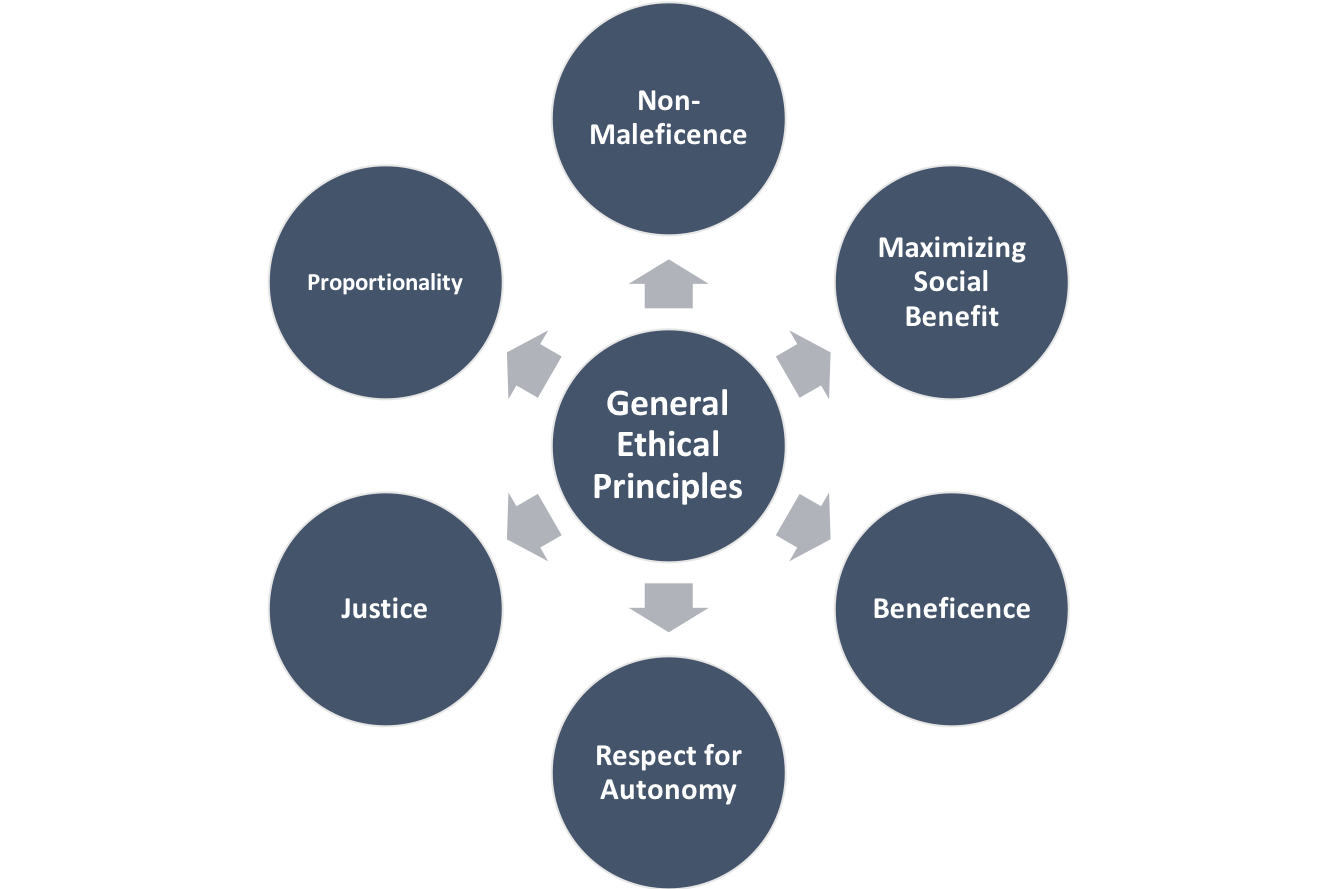
\includegraphics[width=0.5\textwidth,natwidth=850,natheight=550]{figs/ethical-pillars3.png}
        	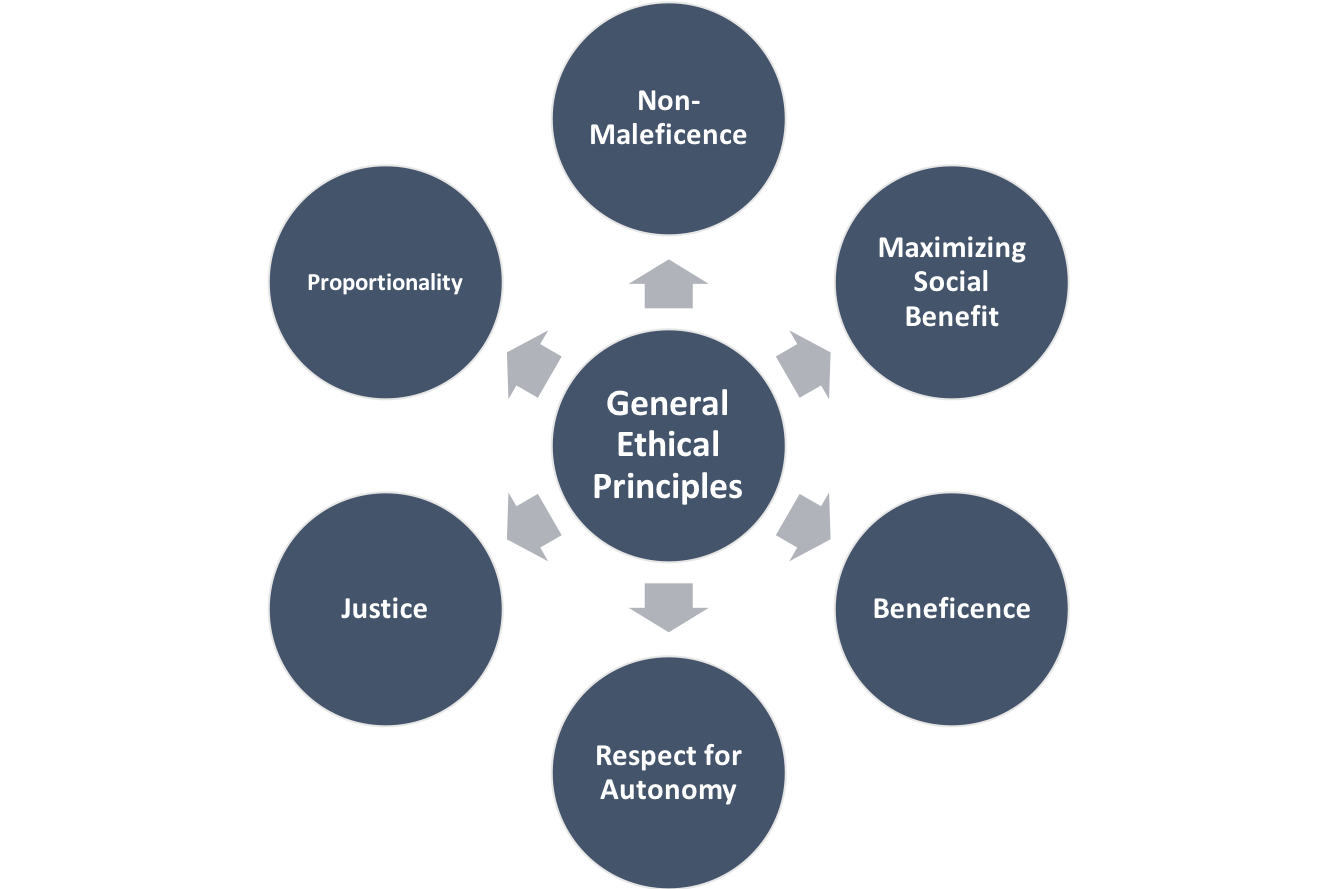
\includegraphics[width=0.5\textwidth]{figs/ethical-pillars3.png}
	\caption{Ethical Principles Applicable to Social Media Setting}
	\label{fig:ethical-pillars}
\end{figure}

Researchers in computer science already make choices in the ordinary course of their studies that draw upon these ethical principles.  Non-maleficence, beneficence, and justice are core principles used to define measures of fairness in machine learning and algorithmic bias. Respect for autonomy and proportionality are foundational concepts within data privacy. Connecting to society and maximizing social good have become themes within subareas of computer science, e.g. data science for social good and AI for social good. As we continue to understand computer science research within the context of different ethical complexities, we must consider harm caused by both processes and entities creating and using developed technologies. Processes include the use of algorithms and models that are biased, lack transparency, or reduce privacy. Measuring algorithmic bias and data exposure are two ways to understand the harm caused by processes. Entities include companies (data collectors), researchers and others (data utilizers) who make decisions that can cause harm to individuals (data generators) or reduce societal benefit. Understanding the role that different entities play in decision making can help researchers better understand their ethical responsibilities when using these types of data. 

\section{Challenges and Foundations}
\label{sec:notation}
Social media challenges are generated by design decisions of each platform, by the types of data users share publicly and privately, and/or the different way researchers and other external groups use the data. Figure \ref{fig:framing} identifies some of these challenges and places them in the context of data privacy and algorithmic bias. In Sections \ref{sec:privacy} and \ref{sec:bias} we will go through these challenges in more detail. 

To start the formalization around some of the concepts we will use, we propose the following mathematical framing of the social media challenges and ethical principles. We will use a security threat model perspective, where an \textit{attack} occurs when ethical considerations are ignored. Let $\mathcal{S} = \{s_1, s_2, \ldots, s_k\}$ be social media sites (platforms). For each social media site, $s_i \in \mathcal{S}$, let $\mathcal{I}_i=\{\mathcal{G}_i, \mathcal{B}_i\}$, where $\mathcal{G}_i = \mathcal{G}^p_i \cup \mathcal{G}^h_i$ is the set of attributes provided by the user and those attributes can be public $\mathcal{G}^p_i$ or hidden $\mathcal{G}^h_i$ and $\mathcal{B}_i$ is the set of attributes auto-generated by  $s_i$. Examples of attributes in $\mathcal{G}_i$ are the user's name and date of birth, while examples of auto-generated attributes in $\mathcal{B}_i$ include the number of friends/followers. Let $\widetilde{\mathcal{I}}_i = \{\widetilde{\mathcal{G}}_i, \widetilde{\mathcal{B}}_i\}$ be the attributes shared by the platforms other than $s_i$, i.e., $\mathcal{S} - \{s_i\}$. 

We define the set of users as $\mathcal{U} = \{u_1, u_2, \cdots, u_n\}$, and define $c(u_j)$ to be a  user class or group that $u_j$ belongs to based on his/her sensitive attributes. User $u_j$ must provide some information when registering on platform $s_i$. The information includes both required and optional fields in  $\mathcal{G}_i$. We denote the user's information as $\mathcal{G}_{i,j}$, and by definition it corresponds to some or all of the attributes captured by platform $\mathcal{G}_i$. 

Social media platforms can use user information to predict values about users. Let $f_i:\mathcal{G}_i \cup \widetilde{\mathcal{G}}_i \rightarrow \mathcal{L}_i$ be a function or model built by social media site $s_i$ which uses information provided by the user $\mathcal{G}_{i,j}$ on $s_i$ and other user information shared by other sites $\widetilde{\mathcal{G}}_i$ to make inferences. $\mathcal{L}_i$ represents attributes learned or inferred by different entities, including social media site $s_i$, and $\mathcal{L}_{i,j}$ are the attributes values inferred for user $u_j$. 

Fundamentally, our security goals are to maintain user privacy, ensure fairness towards individual users $u_j \in \mathcal{U}$ or group of users determined by $c(\cdot)$ (nondiscriminatory behavior), and help users make informed decisions (through transparency). These goals can be mapped to the ethical principles we want to adhere to that were presented in the previous section. There are multiple adversaries in this framing, including social media platforms and other companies $S$, researchers $R$, and other platform users $\mathcal{U}-\{u_j\}$. Let $\mathcal{A}$ be the set of all adversaries, $\mathcal{A} = \mathcal{S} \cup \mathcal{R} \cup \{ \mathcal{U} - \{u_j\} \}$. At a basic level, an adversarial attack occurs when any entity $a \in \mathcal{A}$ uses information in $\mathcal{I}_i$ or $\widetilde{\mathcal{I}}_i$ or $\mathcal{L}_i$ to \textit{violate} one or more of our ethical principles, $\mathcal{E}$. We use the term violate to mean that the ethical consideration is being ignored and/or the expectations of users, in general, are not being met -- a `line' is being crossed.\footnote{This could be modeled as an allowable budget for each ethical consideration.} Let $g: \mathcal{I}_i \cup \widetilde{\mathcal{I}}_i \cup \mathcal{L}_i \rightarrow \mathcal{E}$ be a function that $a_j$ uses to build a model violating ethical principles in $\mathcal{E}$. 

\begin{figure}[tb]
    \centering
    %    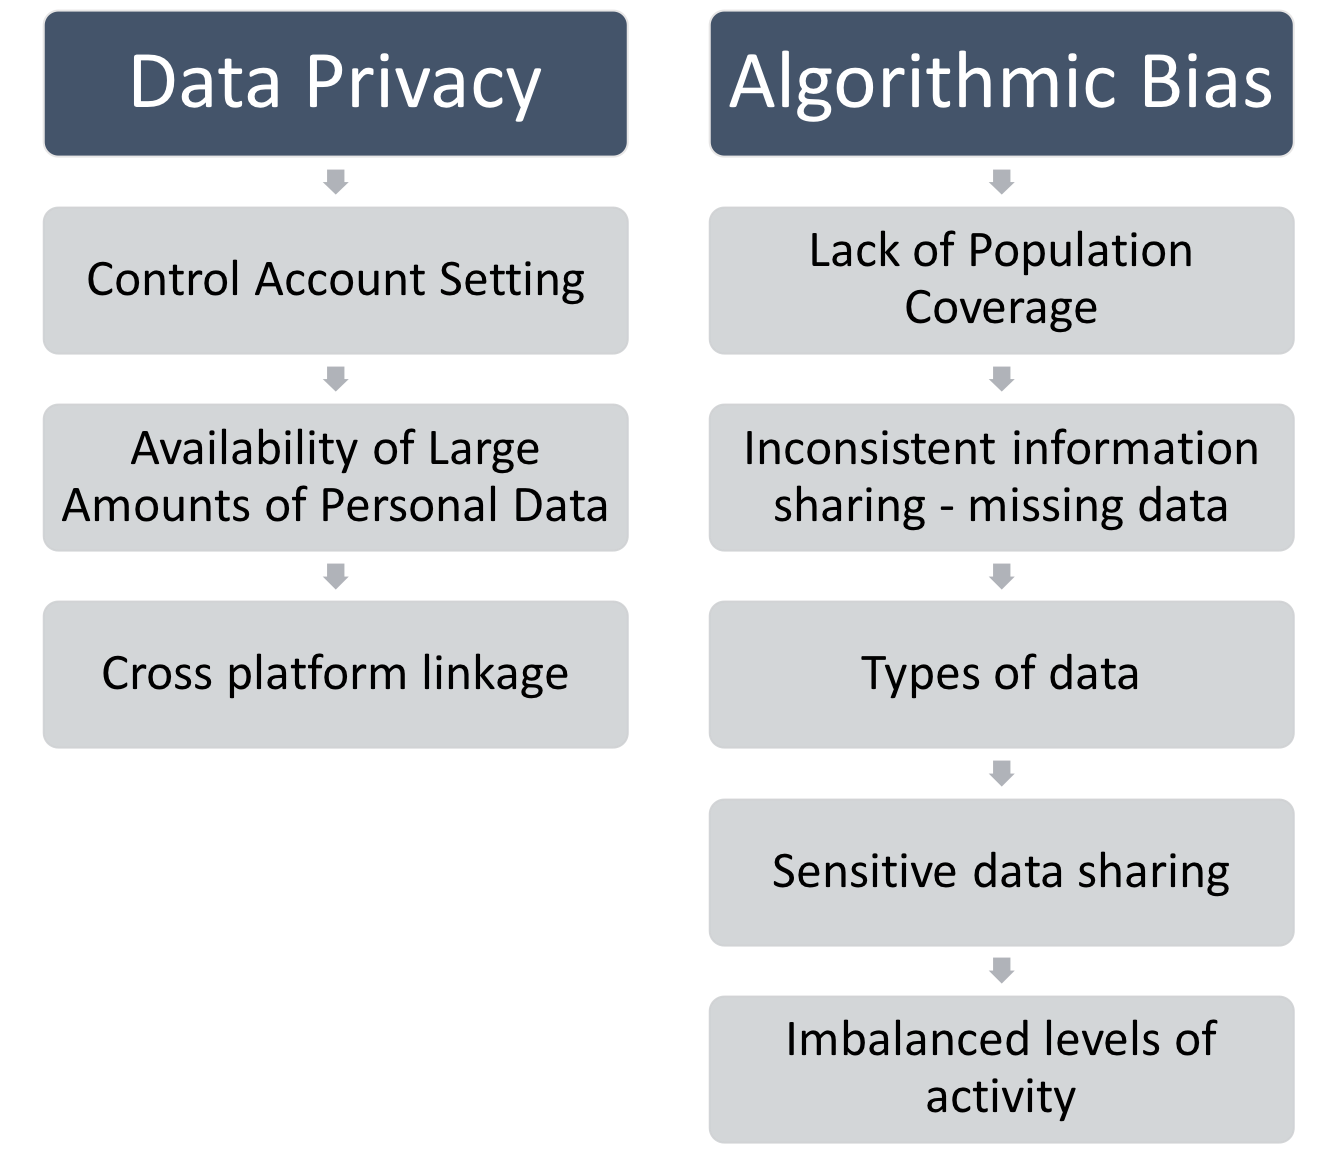
\includegraphics[width=0.35\textwidth,natwidth=890,natheight=730]{figs/sm-challenges2.png}
        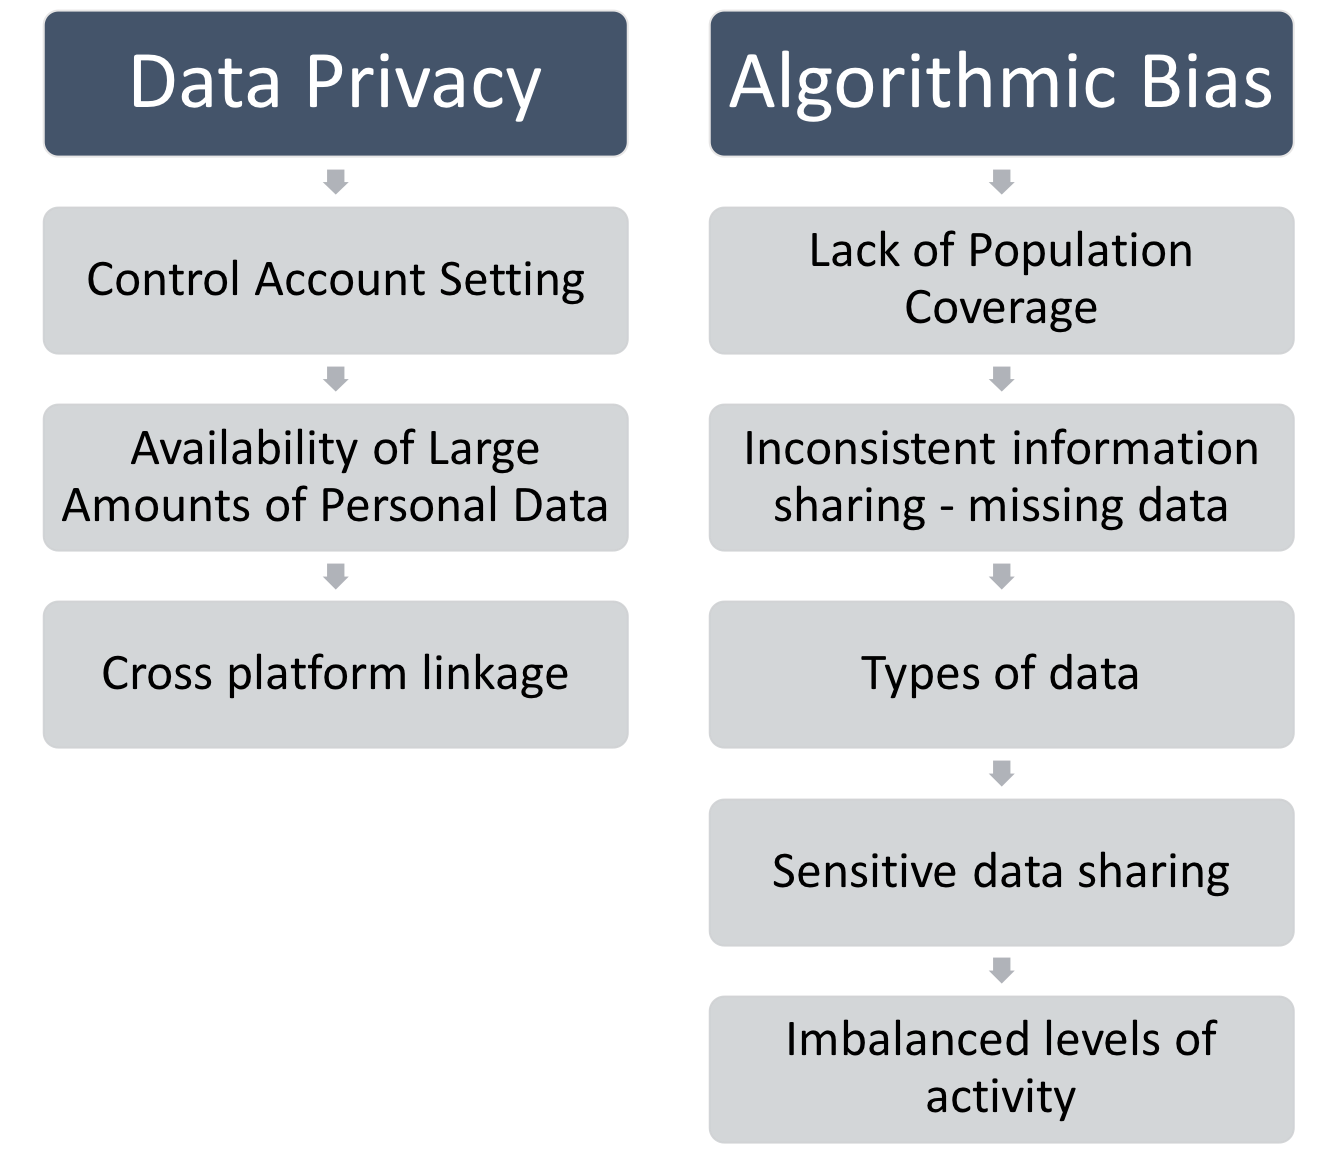
\includegraphics[width=0.35\textwidth]{figs/sm-challenges2.png}
    \caption{Social Media Complexities Within the Contexts of Data Privacy and Algorithmic Bias}
    \label{fig:framing}
\end{figure}
\section{Data Privacy} 
\label{sec:privacy} 
Data privacy research focuses on measuring and reducing the amount of sensitive information that is disclosed. Within the context of social media data, particular attention needs to be paid to disclosure during data collection and data processing. One goal of data privacy research is to develop models and tools that allow users control over their data (and who can access them) and protect each user's privacy preferences and personally identifiable information. Data privacy is a challenging task and it has an even more complicated framing when examined on social media.
For example, social media users freely share large amounts of data that may leak unintended information.  Spontaneous posts and reactions could give insight into sensitive information. Social media companies collect thousands of data points about users, including their photos, their friends, their likes, their activity on the platform,  pages they visit, online purchases, contacts list, and even their location. According to a recent study~\cite{bagrow2019}, advertisers can profile someone with 95\% accuracy using the information from just eight or nine of their friends’ social media accounts. 

Challenges with regards to social media and data privacy arise because users share large amount of information and they have little control over how it is used. This leads to concerns around respect for autonomy, justice proportionality, and maximizing societal benefit.

\subsection{Ability to Control Account Setting}
From an ethical perspective, users should have control of the information they choose to share with the public and with the social media platform. So when an account is setup on a platform, the default setting should always be private ($\mathcal{G}^p_i = \emptyset$ and $\mathcal{G}_i = \mathcal{G}^h_i$), allowing users to make parts of their account public if they choose. They should also not be required to share sensitive information with the platform in order to setup an account. Unfortunately, to promote public discussion and increase community, the default approach for most social media platforms is to setup user accounts as publicly accessible by anyone using the platform, and ask for some sensitive pieces of information during registration. For our example companies, five of the platforms setup public user accounts by default (Snapchat is the one exception). From previous research, we know that part of the reason for this default public setting is that people are not overly concerned with privacy \cite{madden2013teens,SENTHILKUMARN2016114}. Even though concern has risen in recent years \cite{smconcern,smconcern1}, most users do not change their privacy settings to be more private, bringing rise to the ``privacy paradox''~\cite{kokolakis2017,barth2017}. These privacy settings define which features belong to $\mathcal{G}^p_i$ and which to $\mathcal{G}^h_i$, and how successful attacks conducted by adversaries in $\mathcal{A}$ can be.

Given that five of these six platforms are public by default, we begin by trying to understanding how publicly visible user generated data are, what types of information are visible, and whether or not users can make all the publicly visible information private. Table \ref{tab:privacy_setting} summaries the ability of users to control their privacy settings. We organize the table by the subgroup that generates the data fields and the typical functionality on platforms. Users share their data, e.g. account information. Other users ($\mathcal{U}-\{u_i\}$) on the platform can share information about a user $u_i$, e.g. tagging a photo. The last subgroup is about auto-generated fields and platform functionality that expose users information. The table shows that platforms give users control over the data they provide and what other users can do with respect to their data. This is important progress for our industry and likely a result of recent legislation in Europe. However, some platforms fail to let users make data that are generated by the platform private (Twitter, Tiktok, LinkedIn, and Instagram). For example, Twitter users cannot hide their number of followers on their profile page, and LinkedIn users cannot hide their number of connections. 
Platforms sometimes also require users to use functionality that makes use of their shared data. As an example, Instagram does not allow users to turn off personalized ads. 



\begin{table}[]
\caption{Users ability to control their privacy settings}
\label{tab:privacy_setting}
\resizebox{\columnwidth}{!}{%
\begin{tabular}{l lcccccc}
% \begin{tabular}{l lc|c|c|c|c|c}
\toprule
\textbf{Data Generators}                         & \textbf{Data Fields}                                  & \textbf{Facebook} & \textbf{Instagram} & \textbf{Snapchat} & \textbf{Tiktok} & \textbf{Twitter} & \textbf{LinkedIn} \\ \midrule
Individual                       & Profile/account information  & \cmark    & \cmark     & \cmark    & \cmark  & \cmark   & \cmark    \\ \cline{2-8} 
users                          & Posts/story                   & \cmark    & \cmark     & \cmark    & \cmark  & \cmark   & \cmark    \\ \midrule
Other users                        & Tag/mention user             & \cmark    & \cmark     & N/A      & \cmark  & \cmark   & \cmark    \\ \cline{2-8} 
             & Contact user / send comment     & \cmark    & \cmark     & \cmark    & \cmark  & \cmark   & \cmark        \\ \midrule
Platform                        & Personalized ads                       & \cmark    & \xmark     & \cmark    & \cmark  & \cmark   & \cmark    \\ \cline{2-8} 
                & Auto-generated fields                    & \cmark    & \xmark     & N/A      & \xmark  & \xmark   & \xmark    \\ \cline{2-8} 
                        & External partner data sharing                           & \cmark    & \xmark     & \cmark    & \cmark  & \cmark   & \cmark \\ \cline{2-8} 
                        & User search                & \cmark    & \cmark     & \cmark    & \cmark  & \cmark   & \cmark \\ \bottomrule
\end{tabular}%
}
\end{table}


In this context, the two fundamental data privacy concerns are that accounts are public by default ($\mathcal{G}_i \neq \mathcal{G}^h_i$), and not all data fields can be hidden ($\mathcal{G}^p_i \neq \emptyset$). Also, sites are unclear about their default settings or how to change them (lack of transparency).
One problem that arises specifically for researchers and other data utilizers is that some of the data are private, and using the private data for research without user consent can be violate the principles of respect for data ownership and maintenance of privacy. Together, the ethical dilemmas arising from this social media challenge are justice, respect for autonomy, and proportionality. Justice because it is likely that there are subgroups who are structurally speaking more likely not to understand the privacy settings, the defaults, etc., and are therefore, more vulnerable to the manipulation that can occur when the default settings offer no privacy. 
Autonomy is not respected because the default lack of privacy means more data about the users are available to manipulate them through targeted advertisements (commercial, political, or otherwise)~\cite{Susser2018}. Finally, issues of proportionality arise because companies are not being transparent about the default settings or how to change them, leading to more invasive usage of human data and less equitable treatment.
 


\subsection{The Availability of Large Amounts of Personal Data}
Users make decisions about the data they want to share or not share. Figure \ref{fig:req_fields} shows the basic information users need to share to open an account on our example platforms as of November 2020. All the platforms require an email or phone number to register. We see that the number of required fields ranges from three (Twitter) to six (LinkedIn). Five of the six platforms require birthdate (LinkedIn is the one exception), a piece of sensitive information. These required fields along with user activity/post data become the basis for auto-generated fields that lead to 1000s if not 100,000s of new data points for companies. 

\begin{table}[tb]
%\begin{figure}[tb]
\centering
\small
    \caption{Autogenerated fields $\mathcal{B}_i$ for six popular social media platforms}
    \label{tab:autogenerate}
    %    \begin{subtable}{\textwidth}
%  \begin{minipage}{\textwidth}
%        \centering
    %        \caption{Common across platforms}
    \vspace{1em}
(a) Common across platforms\\
    \vspace{1em}
%        \label{tab:autogenerate-a}
            \begin{tabular}{lcccccc} 
            \toprule
Field &   Facebook &   Instagram &   Snapchat &   Tiktok &   Twitter &   LinkedIn \\ \midrule    
Number of friends/followers & \cmark    & \cmark     &          & \cmark  & \cmark   & \cmark    \\\hline
Friend list                 & \cmark    &           &          &        &         & \cmark    \\\hline
Number of followings        & \cmark    & \cmark     &          & \cmark  & \cmark   &          \\\hline
List of followings          & \cmark    & \cmark     &          &        & \cmark   &          \\\hline
List of followers           &          & \cmark     &          &        & \cmark   &          \\\hline
Number of posts             &          & \cmark     &          &        & \cmark   &          \\\hline
Recommended articles/news   & \cmark    &           & \cmark    &        & \cmark   & \cmark    \\\hline
Online events for you       & \cmark    &           &          &        &         & \cmark    \\\hline
Job recommendations         & \cmark    &           &          &        &         & \cmark    \\\hline
Joined on                   &          &           & \cmark    &        & \cmark   &         \\ \bottomrule
            \end{tabular} \\
%  \end{subtable}%
%    \end{minipage}%  
    \vspace{1em}
%    \begin{subtable}{\textwidth}
%    \begin{minipage}{\textwidth}      
        \centering
    \vspace{1em}
       (b) Unique per platform\\
    \vspace{1em}
%        \label{tab:autogenerate-b}
        \begin{tabular}{ccccc} 
\textbf{Facebook}                &  & \textbf{Snapchat}        &  & \textbf{Twitter}                     \\ \cline{1-1} \cline{3-3} \cline{5-5} 
List of events attended &  & Zodiac sign     &  & Signup location             \\
List of reviews         &  &                 &  &                             \\
List of groups          &  & \textbf{Tiktok}          &  & \textbf{LinkedIn}                    \\ \cline{3-3} \cline{5-5} 
Online events for you   &  & Number of likes &  & Number of profile views     \\
                        &  &                 &  & Profiles people also viewed     
        \end{tabular} 
        %    \end{subtable}
%     \end{minipage}
\end{table}
%\end{figure}

Information sharing may also vary across different platforms. Table~\ref{tab:optional} shows the optional fields associated with each platform, both the common ones and the more unique ones that align with the purpose of the platform. 
The one with the highest potential for leakage is LinkedIn since its optional fields capture detailed resume information. Therefore, even though users may feel like they are hidden in a crowd on a single platform, some of this more detailed information makes them more unique if publicly shared. 

Privacy settings only limit what other platform users can see and sometimes, what advertisers can use. The data are still visible to the company and others the company chooses to share the data with. Users in $\mathcal{U}$ have no control over how the company chooses to use these data. For example, even if a user chooses not to share his/her birthdate publicly, the social media platform $s_i \in \mathcal{S}$ can use this information for targeted advertising or to help infer other information of the user such as music interests or political affiliation using $f_i$. Users may be unaware of the types of information being generated and tagged by the platform (see Table \ref{tab:autogenerate}). A 2018 Pew survey showed that 74\% of Facebook users said they did not know that Facebook maintained a list of their traits and interests for targeted advertising and 51\% of users said they were not comfortable that Facebook maintained this list~\cite{FB_targetad}. If users are uncomfortable with companies having this additional information, it is incumbent on researchers to build in mechanisms to conduct research with more transparency than companies. 

Given this situation, ethical concerns related to availability of data center around respect for autonomy. These data are shared without user knowledge, new data are generated without user knowledge, and users do not have the ability to remove data or change some of the generated information. Together these lead to a lack of privacy, transparency, and autonomy. While full control over user information may be a pipe dream without legislation to enforce it, more control and more transparency can be more foundational within computer science research involving social media users. In fact, as researchers, we can build technologies that use different forms of nudging \cite{thaler2009} to encourage users to share less and protect their personal data.
Similar to the previous section, the platforms having such detailed user data that some users are unaware of suggests that justice may also be an ethical consideration since these data can be used to manipulate users and some subpopulations may share data at higher rates than others. 


\subsection{Cross platform linkage}
Different social media platforms attract users for different purposes, including information seeking/sharing and social connection maintenance. It has become increasingly popular for users to have accounts (also called user identities) on multiple social networks~\cite{10.1145/3068777.3068781}. Information shared on different sites can be linked or connected to create \textit{web footprints} of users that expose more information about them. 
Figure~\ref{fig:req_fields} shows a diagram highlighting the common required fields shared by the different platforms. We see that five of the fields are common across two or more platforms. Table~\ref{tab:optional}(a) show the optional fields that users may choose to share. 
Five of the nine optional fields are common across three or more of the six platforms we studied. 
By combining user data $\widetilde{\mathcal{I}}_{i,j}$ from across different sites in $\mathcal{S} - \{s_i\}$ for user $u_j$, features in $\mathcal{G}^h_i$ may be accurately approximated by $\mathcal{L}_i$, even though that information is missing from $\mathcal{G}_{i,j}$, the information provided by $u_j$ on platform $s_i$. Singh and colleagues show the ease with which this type of cross platform linkage attack can be conducted \cite{singh2015}. 


\begin{figure}[tb]
    \centering
    %    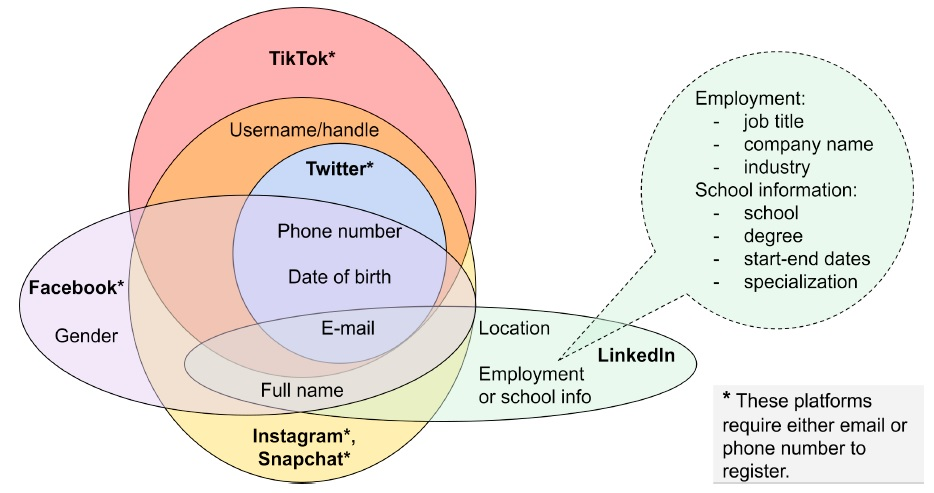
\includegraphics[width=0.7\textwidth,natwidth=650,natheight=300]{figs/req_fields1.png}
        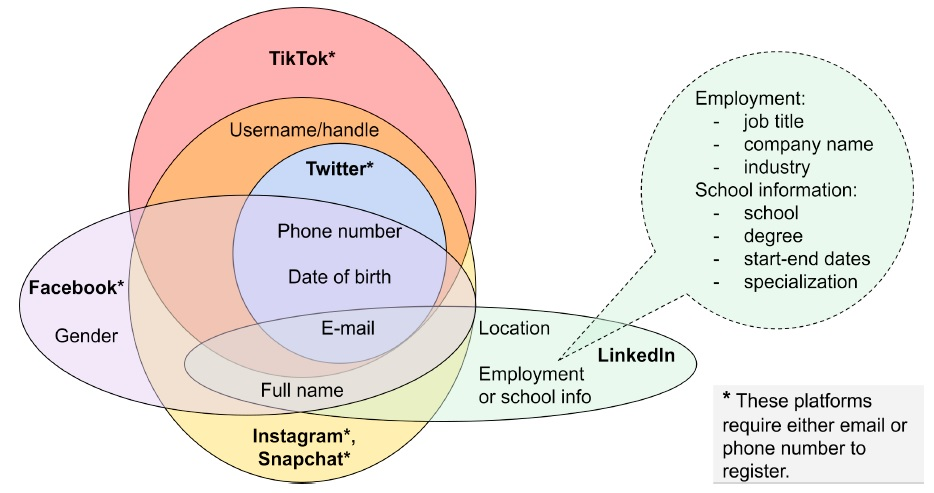
\includegraphics[width=0.7\textwidth]{figs/req_fields1.png}
    \caption{The required fields to set up an account to six popular social media platforms.}
    \label{fig:req_fields}
\end{figure}

Further, when social media data from $s_i \in \mathcal{S}$ are merged across platforms, it can lead to inferring features using $f_i$ that are not shared publicly in ${\mathcal{I}^p_i}$. These additional features may be ones that the user $u_i \in \mathcal{U}$ does not want a researcher or external entity to have. This is a privacy concern if consent is not obtained and/or the benefit of determining the value does not outweigh the harm. Also, privacy issues exist because different demographic subpopulations share attributes across multiple platforms that are more sensitive than other subpopulations, making for easier linking. This leads to a greater privacy loss for some subset of users, who perhaps may belong to more vulnerable communities.

Again, this social media challenge brings us to ethical concerns related to autonomy and justice. 
Autonomy is a concern because the more data available across sites, the more companies and others can identify and specific users. If the targeted population is a vulnerable one, issues of justice also arise. 


\begin{table}[tb]
%\begin{figure}[tb]
\centering
\small
    \caption{Optional fields for six popular social media platforms}
    \label{tab:optional}
    %    \begin{subtable}{\textwidth}
%        \begin{minipage}{\textwidth}

        %        \caption{Common across platforms}
    \vspace{1em}
       (a) Common across platforms\\
    \vspace{1em}
%        \label{tab:optional-a}
            \begin{tabular}{lcccccc} 
            \toprule
Field &   Facebook &   Instagram &   Snapchat &   Tiktok &   Twitter &   LinkedIn \\ \midrule    
Current city       & \cmark &        &  &        & \cmark & \cmark \\ \hline 
School information & \cmark &        &  &        & \cmark & \cmark \\ \hline 
Profile picture    & \cmark & \cmark &  & \cmark & \cmark & \cmark \\ \hline
Cover photo        & \cmark &        &  &        & \cmark & \cmark \\ \hline
Workplace          & \cmark &        &  &        &        & \cmark \\ \hline
Gender             & \cmark & \cmark &  &        &        &        \\ \hline
Bio                & \cmark & \cmark &  &        & \cmark & \cmark \\ \hline
Interested topic   &        &        &  &        & \cmark & \cmark \\ \hline
Website            & \cmark &        &  &        & \cmark &       \\ \bottomrule
            \end{tabular} \\
            %    \end{subtable}%
%    \end{minipage}%
    \vspace{1em}
%    \begin{subtable}{\textwidth}
%    \begin{minipage}{\textwidth}      
        \centering
        %        \caption{Unique per platform}
    \vspace{1em} 
        (b) Unique per platform\\
    \vspace{1em}
%        \label{tab:optionalb}
                             
\begin{tabular}{clclcc}
\textbf{Facebook}   &  & \textbf{Snapchat}            &  & \multicolumn{2}{c}{\textbf{LinkedIn}}    \\ \cline{1-1} \cline{3-3} \cline{5-6} 
Hometown            &  & Bitmoji (personalized emoji) &  & Licences \& certifications & Skills      \\
Relationship status &  &                              &  & List of coursework         & Patents     \\
Family members      &  & \textbf{Tiktok}              &  & Looking for a job          & Industry    \\ \cline{3-3}
                    &  & Profile video                &  & Honors \& awards           & Projects    \\
                    &  &                              &  & Volunteering               & Test scores \\
                    &  &                              &  & Publications               & Languages  
        \end{tabular} 
%    \end{subtable}
%    \end{minipage}
\end{table}


\section{Algorithmic Bias}
\label{sec:bias} 

Researchers from various fields have mined content from social media (that arises organically) to study phenomena traditionally measured using surveys. Within computer science we tend to do this without consent because we view these data as public. But we do need to pause to ask ourselves if the goal of our research is beneficial to the users, the platform, or society more broadly. Should we use such data for inference? Do users realize that their content can be used for various prediction tasks and indirect measurement of different quantities? When is it reasonable for algorithms to use knowledge about membership in a protected subpopulations to infer undisclosed attributes? What is the impact of biased algorithms on individuals? How do we begin to understand the level of harm when we do not have agreed upon ways to measure it? Fairness in machine learning and algorithmic bias are research areas that have begun thinking about some of these questions. Ultimately, using these inferences that were obtained without consent to influence a user's online behavior can be viewed as disregard for a user's actions, which conflicts with the ethical principle of \textit{respect of autonomy}. Making poor quality inferences with or without consent can increase the potential for discrimination (\textit{justice}), potentially manipulation and harm (\textit{beneficence}). When we also consider the potential harm for classes of people as opposed to just individuals, the ethical principle of \textit{societal good maximization} comes into play. We will see that these ethical principles are the primary concerns for each of the social media challenges presented in this section.

Many of the challenges in this section arise because of the differential use of social media. Social media platforms allow their users to communicate with others outside existing social and local boundaries and share with their connections user-generated content. The data generation process is not predictable across all types of users in terms of frequency, types of activity, ways of expression, or topics. People use social media differently and share different aspects of their lives. For some people social media is a social platform. For others it is a professional platform. Different types of engagement (post, comment, share, reaction, or just reading a post) can be driven by similar motivations.  

\subsection{Lack of population coverage}

Inferences from social media data are inherently of unknown representativeness because they come from nonprobability samples that are not designed to cover the population. While non-probability samples are not unique to social media, they are the norm across social media settings. Social media users $\mathcal{U}$ and the different classes/groups they form based on $c(\cdot)$ are not a representative image of the general population, limiting the direct application of many traditional techniques. For example, stratified random sampling techniques used in traditional survey methodology~\cite{deleeuw2008} cannot be directly applied without a proper sampling frame or observed characteristics to help researchers determine the strata in which different individuals fall. This is not to say that social media data are always non-representative. Social media data may end up adequately covering the research topics under study, and thus represent the population accurately, even though the individuals who contributed to the social media corpus are not sampled in a representative way~\cite{schober2016}.
Table \ref{table:platform-demographics} shows the reported populations of each of our example social media sites.  We see that levels of participation on these different sites vary with demographics. LinkedIn and Twitter have more men than women, all of the sites have larger proportions of younger users than older ones, and most have more college educated users than non-college educated.  

Being able to generalize beyond the population of a single platform is important for understanding attitudes and opinions across broader cross-sections of the population. Further, algorithms that are developed for one platform population may need to be adjusted for other populations. Without adjustments, new issues around fairness may arise. Therefore, developing methods for re-weighting populations would increase societal benefit. However, platforms do not share such data about the population distribution in sufficiently regular intervals for researchers to generalize beyond the sample they have without explicitly linking the data to a representative survey. Selection bias has been shown to reduce machine learning fairness in more traditional data sets \cite{suresh2020framework,Kamiran2011DataPT}. This type of bias is exacerbated on social media because we may be unaware of under-representation of subgroups or skews in the data since that information is not released by platforms. This could lead to socially destructive, rather than socially beneficial, knowledge production because of re-enforcement of stereotypes, bias propagation, etc. When we move to high levels of data imbalance, fairness metrics (demographic parity and equality of opportunity) get worse across all levels of privacy~\cite{farrand2020}. Finally, when demographic data is not part of the available data, we cannot verify that algorithms are being fair. As a result, extra caution is necessary when using social media data as direct \cite{de2013predicting} or indirect \cite{10.1145/3292500.3330774}  predictors of social phenomena, and why we need to help build social media benchmarks. 

Ultimately, all of these types of poor quality inferences can lead to concerns with regards to the ethical principles of justice and beneficence. 

\begin{table}[h]
\small
\centering
\caption{Percentage of U.S. adults who use each social media platform by demographics~\cite{sm_demo} }
\label{table:platform-demographics}
\begin{tabular}{cccccc}
\toprule
                      & Facebook & Instagram & LinkedIn & Twitter & Snapchat \\ \midrule
Total                 & 69\%     & 37\%      & 27\%     & 22\%    & 24\%     \\ \midrule
Men                   & 63\%     & 31\%      & 29\%     & 24\%    & 24\% \\ 
Women                 & 75\%     & 43\%      & 24\%     & 21\%    & 24\% \\ \midrule
Ages 18-29          & 79\%     & 67\%      & 28\%     & 38\%    & 62\% \\ 
30-49                 & 79\%     & 47\%      & 37\%     & 26\%    & 25\% \\ 
50-64                 & 68\%     & 23\%      & 24\%     & 17\%    & 9\% \\ 
65+                   & 46\%     & 8\%       & 11\%     & 7\%     & 3\% \\ \midrule
High school or less & 61\%     & 33\%      & 9\%      & 13\%    & 22\%       \\ 
Some college        & 75\%     & 37\%      & 26\%     & 24\%    & 29\%       \\ 
College graduate    & 74\%     & 43\%      & 51\%     & 32\%    & 20\%       \\ \bottomrule
\end{tabular}
\end{table}





\subsection{Types of Data}
Different platforms allow users to generate different types of data, including text (tweets, posts), image and video (profile image, posted photos/videos, and tagged photos/videos), geographic location (geotagged posts/tweets), and relationships/networks (friends and followers). For example, on Twitter the primary mode of communication is text. On Instagram the primary mode is images and on Tiktok the primary mode is video. 

While the prevalence of natural language processing (NLP) and text mining techniques has increased, they are less reliable on short, informal text. Many researchers are applying the same algorithms without making adjustments for the data environment, including understanding the impact of different preprocessing methods on models and adjusting the learning model to account for the noise and bias of social media data. Images have similar issues. While some images are easier to learn from, images shared on social media vary in size, format, and resolution, limiting the reliability of inferences made using these data. Ultimately, algorithms need to be designed or adjusted to compensate for new types of noise prevalent on different social media sites. 


The language used by individuals can reveal demographic characteristics and beliefs. Companies can use images to determine a user's  gender, race, and age even if the user chooses not to share this information. Companies can use geolocation to get user's location and use the location to predict certain characteristics (such as age, gender and income) or even, predict where a user lives or works. For example, researchers have used Twitter user descriptions to infer consumer profiles, predicting attributes such as parental status or if the user is a frequent traveler from the textual content with a precision of between $80\%$ and $92\%$~\cite{hernandez2013}. They also used textual clues, mentions of regional events, Foursquare check-ins, geo-tagged messages, and time zone settings to infer user location with high precision. 

Only recently have researchers begun considering the social impact of natural language processing (NLP)~\cite{hovy2016,blodgett2020}. Text in posts capture how we express ourselves, and they can also capture historical biases and propagate them in the models built~\cite{garg2018,caliskan2017}. For example, word embeddings have been shown to inherit gender bias~\cite{sun2019,bolukbasi2016a,gonen2019}. Additionally, NLP techniques can have difficulty understanding specific dialects within a language~\cite{blodgett2016}. As a result, in the context of social media, dialect speakers’ opinions may be mischaracterized. This is particularly applicable for applications using sentiment analysis and stance. In this context, dialect speakers are discriminated against and possibly even excluded from these models, leading to clear conflicts with regards to the ethical principles of \textit{justice} and \textit{societal good maximisation}\cite{mikal2016}.


\subsection{Sensitive data}
Advances in machine learning have made it possible to infer a large range of attributes about a person. For example, just using information shared in posts, algorithms can infer gender, age, and location with high accuracy.  And when sensitive data are available, e.g. birthdate or race, they will tend to lead to stronger inference predictions. Using these sensitive data for prediction violate the anti-classification definition of fairness, which states that sensitive attributes should not be part of the data used to get a model's outcome. However, an important use of this sensitive information is to ensure group-level and individual-level fairness. 

Because non-sensitive shared personal data of a user or the user's friends can serve as indirect indicator of the user's demographic information, as researchers of data-driven systems, we need to integrate methods to ensure that features generated from personal data are not biased. Additionally, models that do not use sensitive information might still exhibit indirect discrimination, as non-protected attributes may correlate with the protected ones. This is referred to as the ``red-lining'' effect. 

These concerns bring up issues related to the ethical principles of justice and maximizing social benefit. There are many examples of indirect discrimination \cite{oneil2016}. For example, the LinkedIn talent search system returns a list of candidates based on a search query. The system was found to be biased against race and gender and has since been updated \cite{linkedin_unfair}. Another example is Amazon's 2014 hiring application that reviewed resumes to identify top candidates for interviewing. The algorithm was found to be biased against females because the training data (current employee resumes) was heavily biased towards men. Different resume attributes that were being learned by the algorithm were serving as indirect indicators of gender~\cite{dastin_2018}.
These examples are a reminder of the impact of historical data on propagating present day bias. It arises when there is a misalignment between the world as it is and the values or objectives that are encoded and propagated in a model. This bias refers to a concern with the state of the world, and care must be given to this issue on social media, where organic data has inherent biases. If researchers do not correct the biases present in the organic data, they will replicate those biases in the findings, further reinforcing social and cultural inequities. 


\subsection{Partial Information Sharing - Missing data}
People do not fill out all the fields when they sign up for a social media account, revealing different amounts of personal information to others.  Some express their opinions about a larger range of topics than others. Users may share different information with their private network than on their public profile. Ultimately, other than required fields and auto-generated fields, there are very few pieces of information that can be directly obtained across all of the users (see Table \ref{tab:optional}). The result is a significant amount of missing data. 

It is not surprising that companies and researchers have attempted to infer this missing information. However, what happens if the inferred value is incorrect and that value is assumed as accurate for another algorithm? When the data are representative and the algorithms are accurate, the inferences may benefit users. When they are inaccurate and this inaccuracy is further propagated in other algorithms, the harm can be significant.  

The impact of missing values on fairness can be significant. If users choose to not share certain demographic information, how can researchers test if a model is biased against this individual? If we do not have ground truth about the users' sensitive information/features, we cannot verify and guarantee that any models built or conclusions drawn are not biased against (or favoring) a specific set of users. This can be especially problematic when the classification outcome is dependent on users' known features, and these features are correlated to sensitive attributes that are missing. In order to overcome this challenge, some recent research has focused on a pre-processing stage that attempts to ensure that user representation does not indirectly carry any demographic information \cite{10.1177/2053951717743530,Kamiran2011DataPT}. Developing new approaches for measuring fairness when the properties of the underlying data are only partially known is particularly important for social media.

Finally, more generally, we cannot ignore the role missing information plays within data mining and machine learning methods that are deployed on social media.  If missing values are in non-sensitive features, and if the missing values are completely at random, the models being built should be robust. However, if the missing values show bias by exhibiting specific patterns, the models using these data will also be biased \cite{little2019statistical}, raising concerns associated with the ethical principle of justice. 

\subsection{Imbalanced levels of activity}
Users on social media are not equally active. Some are very active, posting continually, while others only browse channels of interest. For example, on Twitter, the top 10\% of the most active tweeters by number of tweets are responsible for 80\% of all tweets created by U.S. adults \cite{pew_twitter}. Levels of engagement can also vary with demographics, campaigns, and across platforms~\cite{perrin2019}. Popular profiles that have many followers/likes tend to post more often than the rest. Figure~\ref{fig:mins_per_day} shows the amount of time users spend on different platforms. While these numbers continues to rise, they vary considerably by demographic. For example, while adults in the US average 38 minutes on Facebook per day, those of ages 16-24 spend three hours on the platform~\cite{whatagraph2020}. Globally, people spent 144 minutes per day on social media. In the United States, people spent 123 minutes per day on social media~\cite{sm_usage}, while they only spent 19 minutes per day exercising~\cite{american_time_spent2020}. In other words, many people are very inclined to spend more time on social media than certain other leisure activity, allowing for potentially better quality inferences; however, the variability is large, requiring researchers to ensure sufficient data are available for stable, repeatable algorithmic development. 
\begin{figure}
    \centering
    %    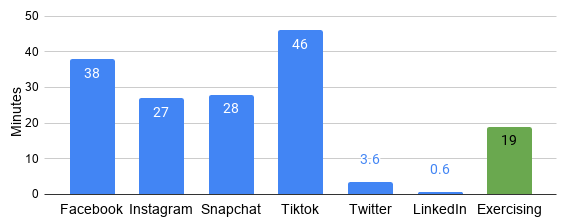
\includegraphics[width=10cm,height = 2cm,natwidth=420,natheight=100]{figs/time_spentExercise.png}
        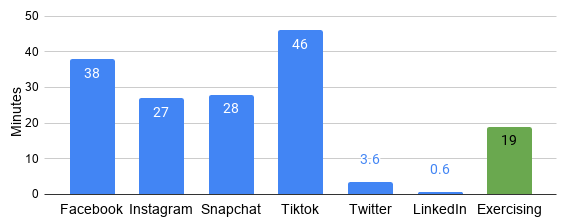
\includegraphics[width=10cm,height = 2cm]{figs/time_spentExercise.png}
    \caption{Average time people spent on each social media platform per day (in minutes).} 
    \label{fig:mins_per_day}
\end{figure}


Also, sometimes researchers only have posts from a particular group or channel and do not know the overall activity level of the users posting on the channel. If the inference is about the content of the post itself, that can be reliable. However, when companies and researchers make inferences about the users, they need to determine the minimum number of posts needed per user for the task. Not doing so will not only lead to measurement validity issues, but also algorithmic bias issues, where accuracy will be higher for those who are more active on social media. Ignoring the levels of user activity when building models reduces the fairness of the model. Inferences made on individuals who post less frequently are likely to be less reliable and more prone to measurement bias, leading to concerns associated with the ethical considerations of non-maleficence and justice.

\section{Transparent Computing}
\label{sec:transparency}
Users are inundated with huge volumes of information and a large number of choices. Social media applications have only made this more challenging. Users may be unaware of the data that are being shared or used by different platforms, and if they are aware, they may not understand how the platforms are using the data or how to make adjustments to their data sharing preferences. For example, many users on Facebook are not aware that people outside of their network of friends can see their account information \cite{orito_2014,FB_targetad}.
At the same time, computational models continue to increase in complexity, making it harder for researchers and programmers to understand the impact of different data features on developed inference models. 

As machine learning models continue to influence human behavior and drive our decision making, the topic of transparency continues to reoccur within this context. Transparency is being discussed as a synonym for interpretability, i.e. an explanation of the model, to ensure a model's outcomes are understandable and fair to humans. However, transparent/interpretable models are only one piece of the learning process, or more broadly, of a computational model. Algorithmic fairness and privacy capture important desired characteristics of an implemented computing model with respect to ethical concerns. However, we argue that these concepts capture only a part of computational transparency. The complexity of the data and the software require use to to reimagine data and software transparency. This includes transparency during data collection, data preprocessing, model design and implementation, and model outputs.  When a system and the data within the system are transparent across all its components, it is not only easier to understand the system, but it also makes it easier to determine the components most vulnerable to ethical attacks. 

Having more transparency throughout the software development lifecycle is not a new idea. However, exposing both the inputs and the data usages throughout will enable researchers to connect computation to the ethical principles defined in Section \ref{sec:ethics}. Toward that end, we define \textit{transparent computing} to be the study of transparency mechanisms for computing. Transparency is fundamental to all of the mentioned ethical principles. The pillars of transparent computing would include the following: (1) ensuring that coded policy constraints, including ethical considerations, related to user data are transparent, (2) ensuring that the data being used by algorithms are transparent,\footnote{In cases where data values cannot be shared, measures can be shared to inform researchers about the properties of the data.} (3) ensuring that the models used to make inferences are transparent, and when possible interpretable, (4) ensuring that the reliability of the algorithm in terms of accuracy and fairness are transparent, and (5) ensuring that generalizability and limitations of model usage and analysis are clear. Without embedding principles of transparency into our problem formulation, model construction, and shared results, quantifying and measuring the effectiveness of our algorithms and privacy mechanisms with regards to ethical principles will not be straightforward. Our field will continue to have to grapple with the inconsistency between what we do and what makes ethical sense to do.

\section{Final Thoughts}
While some of the complexities we identify are are not novel and have been issues associated with traditional data sources, e.g. surveys and administrative data, the social media context is new and requires us to rethink our approach for addressing these complexities, while understanding the ethical implications of our solutions. 
%Given the complexities specific to social media, what are the ethical conundrums that are emerging as they relate to algorithmic bias and data privacy? 
How do we ensure that algorithms and tools that we design are fair, transparent, and privacy preserving to humans, while also being beneficial to society? The irregular noise in social media data, the inherent bias in features generated from the data, and the lack of understanding of the representativeness of social media platforms make it harder to develop correct and sound algorithmic, machine learning, and privacy solutions. And that difficulty is even more challenging when we throw ethics into the mix. As computer science researchers, we are at an important crossroad. We can continue to build algorithms and tools that companies use to exploit user data. Or we can understand that users who share their data freely with companies need researchers to develop guidelines for use of these data, for design of algorithms that consider transparency and fairness, and for technologies that protect user data and use user data responsibly. 

While this area is emerging and guidelines are still be developed, there are best practices that have been identified in other disciplines that we can begin to follow. First, if possible, researchers should use public data and make clear in the study how the data are collected. If the data are private, researchers can conduct thought exercises that work through the potential ethical considerations and potential user/societal harms to ensure that the use of private data is warranted. If a decision is made to move forward, the researchers should get consent to use the data and give users options to decline and leave the study at any point. When inferring new values or developing new models, researchers can compute not only measures of accuracy, but also measures of fairness. Finally, researchers should continue to make data, models, and results transparent and reproducible. By designing algorithms and technologies with ethical considerations from the outset, perhaps we can begin to create a new breed of computer science that deliberately connects our computation work to social responsibility.
\section*{Acknowledgements}
This research is funded by National Science Foundation awards \#1934925 and \#1934494, the National Collaborative on Gun Violence Research (NCGVR), the Fritz Family Fellowship, and the Massive Data Institute (MDI) at Georgetown University. We thank our funders for supporting this research. 

\begin{thebibliography}{10}
\begin{small}
\itemsep=1pt


\bibitem{american_time_spent2020}
American {Time} {U}se {S}urvey {News} {Release} - 2019 {Results} (2020),
  https://www.bls.gov/news.release/archives/atus \_06252020.htm

\bibitem{bagrow2019}
Bagrow, J.P., Liu, X., Mitchell, L.: Information flow reveals prediction limits
  in online social activity. Nature Human Behaviour  \textbf{3}(2),  122--128
  (Feb 2019)

\bibitem{barth2017}
Barth, S., De~Jong, M.D.: The privacy paradox--{Investigating} discrepancies
  between expressed privacy concerns and actual online behavior–{A}
  systematic literature review. Telematics and informatics  \textbf{34}(7),
  1038--1058 (2017)

\bibitem{blodgett2020}
Blodgett, S.L., Barocas, S., Daumé~III, H., Wallach, H.: Language
  ({Technology}) is {Power}: {A} {Critical} {Survey} of  ``{Bias}" in {NLP}.
  arXiv preprint arXiv:2005.14050  (2020)

\bibitem{blodgett2016}
Blodgett, S.L., Green, L., O'Connor, B.: Demographic dialectal variation in
  social media: {A} case study of {African}-{American} {English}. arXiv
  preprint arXiv:1608.08868  (2016)

\bibitem{bolukbasi2016a}
Bolukbasi, T., Chang, K.W., Zou, J.Y., Saligrama, V., Kalai, A.T.: Man is to
  computer programmer as woman is to homemaker? debiasing word embeddings. In:
  Advances in neural information processing systems (2016)

\bibitem{caliskan2017}
Caliskan, A., Bryson, J.J., Narayanan, A.: Semantics derived automatically from
  language corpora contain human-like biases. Science  \textbf{356}(6334),
  183--186 (2017)

\bibitem{10.1145/3376898}
Chouldechova, A., Roth, A.: A snapshot of the frontiers of fairness in machine
  learning. Commun. ACM  \textbf{63}(5),  82-89 (Apr 2020)

\bibitem{dastin_2018}
Dastin, J.: Amazon scraps secret ai recruiting tool that showed bias against
  women (2018),
  https://www.reuters.com/article/us-amazon-com-jobs-automation-insight/amazon-scraps-secret-ai-recruiting-tool-that-showed-bias-against-women-idUSKCN1MK08G

\bibitem{linkedin_unfair}
Day, M.: How linkedin's search engine may reflect a gender bias (Aug 2016),
  https://www.seattletimes.com/business/microsoft/how-linkedins-search-engine-may-reflect-a-bias

\bibitem{de2013predicting}
De~Choudhury, M., Gamon, M., Counts, S., Horvitz, E.: Predicting depression via
  social media. Icwsm  \textbf{13},  1--10 (2013)

\bibitem{deleeuw2008}
De~Leeuw, E.D., Hox, J.J., Dillman, D.A.: International handbook of survey
  methodology. Taylor \& Francis Group/Lawrence Erlbaum Associates (2008)

\bibitem{farrand2020}
Farrand, T., Mireshghallah, F., Singh, S., Trask, A.: Neither private nor fair:
  Impact of data imbalance on utility and fairness in differential privacy.
  arXiv preprint arXiv:2009.06389  (2020)

\bibitem{garg2018}
Garg, N., Schiebinger, L., Jurafsky, D., Zou, J.: Word embeddings quantify 100
  years of gender and ethnic stereotypes. Proceedings of the National Academy
  of Sciences  \textbf{115}(16),  E3635--E3644 (2018)

\bibitem{gonen2019}
Gonen, H., Goldberg, Y.: Lipstick on a pig: {Debiasing} methods cover up
  systematic gender biases in word embeddings but do not remove them. arXiv
  preprint arXiv:1903.03862  (2019)

\bibitem{us1979belmont}
of~Health, U.D., Services, H., et~al.: The belmont report: Office of the
  secretary, ethical principles and guidelines for the protection of human
  subjects of research, the national commission for the protection of human
  subjects of biomedical and behavioral research (1979)

\bibitem{sm_usage}
Henderson, G.: How much time does the average person spend on social media?
  (Aug 2020),
  https://www.digitalmarketing.org/blog/how-much-time-does-the-average-person-spend-on-social-media

\bibitem{hernandez2013}
Hernandez, M., Hildrum, K., Jain, P., Wagle, R., Alexe, B., Krishnamurthy, R.,
  Stanoi, I.R., Venkatramani, C.: Constructing consumer profiles from social
  media data. In: {IEEE} {International} {Conference} on {Big} {Data}. pp.
  710--716. IEEE (2013)

\bibitem{FB_targetad}
Hitlin, P., Rainie, L.: Facebook algorithms and personal data (Jan 2019),
  https://www.pewresearch.org/internet/2019/01/16/facebook-algorithms-and-personal-data/

\bibitem{hovy2016}
Hovy, D., Spruit, S.L.: The social impact of natural language processing. In:
  Proceedings of the 54th {Annual} {Meeting} of the {Association} for
  {Computational} {Linguistics} ({Volume} 2: {Short} {Papers}). pp. 591--598
  (2016)

\bibitem{pew_twitter}
Hughes, A., Wojcik, S.: Key takeaways from our new study of how americans use
  twitter (April 2019),
  https://www.pewresearch.org/fact-tank/2019/04/24/key-takeaways-from-our-new-study-of-how-americans-use-twitter

\bibitem{Kamiran2011DataPT}
Kamiran, F., Calders, T.: Data preprocessing techniques for classification
  without discrimination. Knowledge and Information Systems  \textbf{33},
  1--33 (2011)

\bibitem{kammourieh2017}
Kammourieh, L., Baar, T., Berens, J., Letouzé, E., Manske, J., Palmer, J.,
  Sangokoya, D., Vinck, P.: Group privacy in the age of big data. In: Group
  {Privacy}, pp. 37--66. Springer (2017)

\bibitem{kokolakis2017}
Kokolakis, S.: Privacy attitudes and privacy behaviour: {A} review of current
  research on the privacy paradox phenomenon. Computers \& security
  \textbf{64},  122--134 (2017)

\bibitem{Kramer8788}
Kramer, A.D.I., Guillory, J.E., Hancock, J.T.: Experimental evidence of
  massive-scale emotional contagion through social networks. Proceedings of the
  National Academy of Sciences  \textbf{111}(24),  8788--8790 (2014)

\bibitem{Lipworth2017}
Lipworth, W., Mason, P., Kerridge, I., Ioannidis, J.: Ethics and epistemology
  in big data research. Journal of Bioethical Inquiry  \textbf{14} (2017)

\bibitem{little2019statistical}
Little, R.J., Rubin, D.B.: Statistical analysis with missing data, vol.~793.
  John Wiley \& Sons (2019)

\bibitem{luka2017}
Luka, M.E., Millette, M., Wallace, J.: A feminist perspective on ethical
  digital methods. Internet research ethics for the social age p.~21 (2017)

\bibitem{10.1080/15265161.2019.1602190}
Lynch, H.F., Largent, E.A.: Mountains and molehills when using social media as
  a research support tool. The American Journal of Bioethics  \textbf{19}(6),
  64--66 (2019)

\bibitem{madden2013teens}
Madden, M., Lenhart, A., Cortesi, S., Gasser, U., Duggan, M., Smith, A.,
  Beaton, M.: Teens, social media, and privacy. Pew Research Center
  \textbf{21}(1055),  2--86 (2013)

\bibitem{mikal2016}
Mikal, J., Hurst, S., Conway, M.: Ethical issues in using {Twitter} for
  population-level depression monitoring: a qualitative study. BMC medical
  ethics  \textbf{17}(1), ~22 (2016)

\bibitem{7515114}
{O'Leary}, D.E.: Ethics for big data and analytics. IEEE Intelligent Systems
  \textbf{31}(4),  81--84 (2016)

\bibitem{oneil2016}
O'neil, C.: Weapons of math destruction: How big data increases inequality and
  threatens democracy. Broadway Books (2016)

\bibitem{orito_2014}
Orito, Y., Fukuta, Y., Murata, K.: I will continue to use this nonetheless:
  Social media survive users' privacy concerns. International Journal of
  Virtual Worlds and Human Computer Interaction  \textbf{2},  92--107 (12 2014)

\bibitem{socialdilemma}
Orlowski, J.: The social dilemma. Exposure Labs (2020)

\bibitem{smconcern}
Perrin, A.: Americans are changing their relationship with facebook (Sep 2018),
  https://www.pewresearch.org/fact-tank/2018/09/05/americans-are-changing-their-relationship-with-facebook/

\bibitem{perrin2019}
Perrin, A., Andreson, M.: Share of {U}.{S}. adults using social media,
  including {Facebook}, is mostly unchanged since 2018 (Apr 2019),
  https://www.pewresearch.org/fact-tank/2019/04/10/share-of-u-s-adults-using-social-media-including-facebook-is-mostly-unchanged-since-2018/

\bibitem{sm_demo}
Social media fact sheet (Jun 2019),
  https://www.pewresearch.org/internet/fact-sheet/social-media/

\bibitem{10.1177/1556264619901215}
Samuel, G., Buchanan, E.: Guest editorial: Ethical issues in social media
  research. Journal of Empirical Research on Human Research Ethics
  \textbf{15}(1-2),  3--11 (2020)

\bibitem{samuel2019}
Samuel, G., Derrick, G.E., van Leeuwen, T.: The {Ethics} {Ecosystem}:
  {Personal} {Ethics}, {Network} {Governance} and {Regulating} {Actors}
  {Governing} the {Use} of {Social} {Media} {Research} {Data}. Minerva
  \textbf{57}(3),  317--343 (Sep 2019)

\bibitem{schober2016}
Schober, M.F., Pasek, J., Guggenheim, L., Lampe, C., Conrad, F.G.: Social
  {Media} {Analyses} for {Social} {Measurement}. Public Opinion Quarterly
  \textbf{80}(1),  180--211 (2016)

\bibitem{SENTHILKUMARN2016114}
{Senthil Kumar N}, {Saravanakumar K}, {Deepa K}: On privacy and security in
  social media : A comprehensive study. Procedia Computer Science  \textbf{78},
   114 -- 119 (2016), international Conference on Information Security \&
  Privacy 2015

\bibitem{10.1145/3068777.3068781}
Shu, K., Wang, S., Tang, J., Zafarani, R., Liu, H.: User identity linkage
  across online social networks: A review. SIGKDD Explor. Newsl.
  \textbf{18}(2),  5–17 (Mar 2017)

\bibitem{10.1145/3292500.3330774}
Singh, L., Wahedi, L., Wang, Y., Wei, Y., Kirov, C., Martin, S., Donato, K.,
  Liu, Y., Kawintiranon, K.: Blending noisy social media signals with
  traditional movement variables to predict forced migration. p. 1975–1983.
  KDD '19, Association for Computing Machinery, New York, NY, USA (2019)

\bibitem{singh2015}
Singh, L., Yang, G.H., Sherr, M., Hian{-}Cheong, A., Tian, K., Zhu, J., Zhang,
  S.: Public information exposure detection: Helping users understand their web
  footprints. In: {IEEE/ACM} International Conference on Advances in Social
  Networks Analysis and Mining (ASONAM). pp. 153--161. Paris, France (August
  2015)

\bibitem{smconcern1}
New duckduckgo research shows people taking action on privacy (Oct 2019),
  https://spreadprivacy.com/people-taking-action-on-privacy/

\bibitem{sun2019}
Sun, T., Gaut, A., Tang, S., Huang, Y., ElSherief, M., Zhao, J., Mirza, D.,
  Belding, E., Chang, K.W., Wang, W.Y.: Mitigating gender bias in natural
  language processing: {Literature} review. arXiv preprint arXiv:1906.08976
  (2019)

\bibitem{suresh2020framework}
Suresh, H., Guttag, J.V.: A framework for understanding unintended consequences
  of machine learning (2020)

\bibitem{b88a5a9441354a02ac5b105291fff917}
Susser, D.: Information privacy and social self-authorship. Techne: Research in
  Philosophy and Technology  \textbf{20}(3),  216--239 (2016), copyright:
  Copyright 2017 Elsevier B.V., All rights reserved.

\bibitem{Susser2018}
Susser, D., Roessler, B., Nissenbaum, H.: Online manipulation: Hidden
  influences in a digital world. SSRN Electronic Journal  (01 2018)

\bibitem{TANGWA2009S2}
Tangwa, G.B.: Ethical principles in health research and review process. Acta
  Tropica  \textbf{112},  S2 -- S7 (2009), health Research in Africa: Ethical
  and Practical Challenges

\bibitem{10.1177/1747016117738559}
Taylor, J., Pagliari, C.: Mining social media data: How are research sponsors
  and researchers addressing the ethical challenges? Research Ethics
  \textbf{14}(2),  1--39 (2018)

\bibitem{thaler2009}
Thaler, R.H., Sunstein, C.R.: Nudge: Improving decisions about health, wealth,
  and happiness. Penguin (2009)

\bibitem{10.1080/15265161.2019.1611278}
Torous, J., Ungar, L., Barnett, I.: Expanding, augmenting, and operationalizing
  ethical and regulatory considerations for using social media platforms in
  research and health care. The American Journal of Bioethics  \textbf{19}(6),
  ~4--6 (2019)

\bibitem{Turoldo2008}
Turoldo, F.: Responsibility as an ethical framework for public health
  interventions. American journal of public health  \textbf{99},  1197--202 (11
  2008)

\bibitem{10.1177/2053951717743530}
Veale, M., Binns, R.: Fairer machine learning in the real world: Mitigating
  discrimination without collecting sensitive data. Big Data \& Society
  \textbf{4}(2),  2053951717743530 (2017)

\bibitem{fb_Analytica}
Wagner, K.: Here’s how facebook allowed cambridge analytica to get data for
  50 million users (Mar 2018),
  https://www.vox.com/2018/3/17/17134072/facebook-cambridge-analytica-trump-explained-user-data

\bibitem{whatagraph2020}
How much time do people spend on social media (11 insights) {\textbar} {Blog}
  {\textbar} {Whatagraph} (Aug 2020),
  https://whatagraph.com/blog/articles/how-much-time-do-people-spend-on-social-media

\bibitem{ozkula2020}
Özkula, S.M.: The {Issue} of ``{Context}": {Data}, {Culture}, and
  {Commercial} {Context} in {Social} {Media} {Ethics}. Journal of Empirical
  Research on Human Research Ethics  \textbf{15}(1-2),  77--86 (2020)
\end{small}
\end{thebibliography}

%
% BibTeX users please use
% \bibliographystyle{}
% \bibliography{}


\end{document}





\end{article}
%
%\makeatletter
%\renewcommand{\AB@affillist}{}
%\renewcommand{\AB@authlist}{}
%\setcounter{authors}{0}
%\makeatother
%
\begin{article}
{Taming Technical Bias in Machine Learning Pipelines}
{Sebastian Schelter and Julia Stoyanovich}
\graphicspath{{submissions/SchelterStoyanovich_final/}}
\documentclass[11pt]{article} 
\usepackage[utf8]{inputenc}

\usepackage{deauthor,times}
\usepackage{graphicx}
\usepackage{hyperref}
\usepackage{amsfonts,amsmath}
\usepackage{enumitem}
\usepackage{xspace} 
\usepackage{xcolor}

\newcommand*{\rf}{\textsf{Ranking Facts}\xspace}
\newcommand*{\eg}{e.g.,\xspace}
\newcommand*{\ie}{i.e.,\xspace}
\newcommand{\etal}{et al.\xspace}

\newcommand{\fairprep}{\stt{FairPrep}\xspace}
\newcommand{\aif}{\stt{AIF360}\xspace}
\newcommand{\sklearn}{\stt{scikit-learn}\xspace}
\newcommand{\pandas}{\stt{pandas}\xspace}
\newcommand{\mlinspect}{\stt{mlinspect}\xspace}
\newcommand{\deequ}{\stt{Deequ}\xspace}


\newcommand{\adult}{\texttt{adult}\xspace}
\newcommand{\german}{\texttt{germancredit}\xspace}
\newcommand{\propublica}{\texttt{propublica}\xspace}
\newcommand{\ricci}{\texttt{ricci}\xspace}


\newcommand{\header}[1]{\vspace{1mm}\noindent\textbf{#1}.}
\newcommand{\headerl}[1]{\vspace{1mm}\noindent\textit{#1}.}

\newcommand{\rev}[1]{#1}
\newcommand{\revtammo}[1]{#1}

\newcommand{\todo}[1]{\textcolor{purple}{TODO: #1}}

\usepackage{tikz}
\newcommand*\circled[1]{\tikz[baseline=(char.base)]{\node[shape=circle,fill=black,draw,inner sep=0.6pt] (char) {\textcolor{white}{\footnotesize \textbf{#1}}};}}

\newcommand{\julia}[1]{\textcolor{teal}{[Julia: #1]}}
\newcommand{\sebastian}[1]{\textcolor{blue}{[Julia: #1]}}

\newcommand{\shref}[2]{{\footnotesize\href{#1}{#2}}}
\newcommand{\surl}[1]{{\footnotesize\url{#1}}}
\newcommand{\stt}[1]{{\footnotesize\texttt{#1}}}

\usepackage[T1]{fontenc}
\usepackage{beramono}
\usepackage{listings}
\usepackage{xcolor}

\definecolor{dkgreen}{rgb}{0,0.6,0}
\definecolor{gray}{rgb}{0.5,0.5,0.5}
\definecolor{mauve}{rgb}{0.58,0,0.82}

\lstdefinestyle{myScalastyle}{
  frame=tb,
  language=scala,
  aboveskip=3mm,
  belowskip=3mm,
  showstringspaces=false,
  columns=flexible,
  basicstyle={\scriptsize\ttfamily},
  numbers=none,
  numberstyle=\tiny\color{gray},
  keywordstyle=\color{blue},
  commentstyle=\color{dkgreen},
  stringstyle=\color{mauve},
  frame=single,
  breaklines=true,
  breakatwhitespace=true,
  tabsize=3,
}

\begin{document}

\title{Taming Technical Bias in Machine Learning Pipelines
\footnote{This work was supported in part by NSF Grants No. 1926250, 1934464, and 1922658, and by Ahold Delhaize. All content represents the opinion of the authors, which is not necessarily shared or endorsed by their respective employers and/or sponsors.}}

\author{
Sebastian Schelter\\
University of Amsterdam \& Ahold Delhaize\\
Amsterdam, The Netherlands \\
s.schelter@uva.nl
\and
 Julia Stoyanovich \\
New York University \\
New York, NY, USA \\
stoyanovich@nyu.edu}

\maketitle

\begin{abstract}
Machine Learning (ML) is commonly used to automate decisions in domains as varied as credit and lending,  medical diagnosis, and  hiring.  These decisions are consequential, imploring us to carefully balance the benefits of efficiency with the potential risks.   Much of the conversation about the risks centers around bias --- a term that is used by the technical community ever more frequently but that is still poorly understood. 
In this paper we focus on technical bias --- a type of bias that has so far received limited attention and that the data engineering community is well-equipped to address. We discuss dimensions of technical bias that can arise through the ML lifecycle, particularly when it's due to preprocessing decisions or post-deployment issues.  We present results of our recent work, and discuss future research directions. Our over-all goal is to support the development of systems that  expose the knobs of responsibility to data scientists, allowing them to detect instances of technical bias and to mitigate it when possible.
\end{abstract}

\section{Introduction}
\label{sec:intro}

Machine Learning (ML) is increasingly used to automate  decisions that impact people's lives, in domains as varied as credit and lending,  medical diagnosis, and  hiring. The risks and opportunities arising from the wide-spread use of predictive analytics are garnering much attention from policy makers, scientists, and the media.  Much of this conversation centers around \emph{bias} --- a term that is used by the technical community ever more frequently but that is still poorly understood. 

In their seminal 1996 paper, Friedman and Nissenbaum identified three types of bias that can arise in computer systems: pre-existing, technical, and emergent ~\cite{DBLP:journals/tois/FriedmanN96}.    We briefly discuss these in turn, see Stoyanovich~\etal~\cite{DBLP:journals/pvldb/StoyanovichHJ20} for a more comprehensive  overview.

\begin{itemize}[leftmargin=*]
\item \emph{Pre-existing  bias} has its origins in society.  In ML applications, this type of bias often exhibits itself in the input data; detecting and mitigating it is the subject of much research under the heading of algorithmic fairness~\cite{DBLP:journals/cacm/ChouldechovaR20}. Importantly, the presence or absence of pre-existing bias cannot be scientifically verified, but rather is postulated based on a belief system~\cite{DBLP:journals/corr/FriedlerSV16,DBLP:conf/fat/HeidariLGK19}. Consequently, the effectiveness --- or even the validity --- of a technical attempt to mitigate pre-existing bias is predicated on that belief system.

\item \emph{Technical bias} arises due to the operation of the technical system itself, and can amplify pre-existing bias.  The bad news is that, as we argue in the remainder of this paper, the risks of introducing technical bias in ML pipelines abound. The good news is that, unlike with pre-existing bias, there is no ambiguity about whether a technical fix should be attempted: if technical systems we develop are introducing bias, then we should be able to instrument these systems to measure it and understand its cause. It may then be possible to mitigate this bias and to check whether the mitigation was effective.

\item \emph{Emergent bias}   arises in the context of use of the technical system. In Web ranking and recommendation in e-commerce, a prominent example is ``rich-get-richer'': searchers tend to trust the systems to indeed show them the most suitable items at the top positions, which in turn shapes a searcher's idea of a satisfactory answer.

\end{itemize}

In this paper, we focus on technical bias,  --- a type of bias that has so far received limited attention, particularly when it's due to preprocessing decisions or post-deployment issues, and that the data engineering community is well-equipped to address.  Our over-all goal is to support the development of systems that \emph{expose the knobs of responsibility to data scientists}, allowing them to detect instances of technical bias, and to mitigate it when possible.


\header{Running example} We illustrate the need for taming technical bias with an example from the medical domain. Consider a data scientist who implements a Python pipeline that takes demographic and clinical history data as input, and trains a classifier to identify patients at risk for serious complications. Further, assume that the data scientist is under a legal obligation to ensure that the resulting ML model works equally well for patients across different gender and age groups.  This obligation is operationalized as an intersectional fairness criterion, requiring equal false negatives rates for groups of patients identified by a combination of gender and age group. 

Consider Ann, a data scientist who is developing this classifier. Following her company's best practices, Ann will start by splitting her dataset into training, validation, and test sets. Ann will then use \pandas, \sklearn~\cite{Pedregosa2011}, and their accompanying data transformers to explore the data and implement data preprocessing, model selection, tuning, and validation. Ann starts preprocessing by computing value distributions and correlations for the features in her dataset, and by identifying missing values. She will fill these in using a default interpolation method in scikit-learn, replacing missing values with the mode value for that feature.  Finally, following the accepted best practices at her company, Ann implements model selection and hyperparameter tuning. As a result of this step, Ann will select a classifier that shows acceptable performance according to her company's standard metrics: it has sufficient accuracy, while also exhibiting sufficiently low variance. 
When Ann considers the accuracy of her classifier closely, she observes a disparity: accuracy is lower for middle-aged women. Ann is now faced with the challenge of figuring out why this is the case, whether any of her technical choices during pipeline construction contributed to this model bias, and what she can do to mitigate this effect. We will revisit this example, and also discuss issues that may arise after the model is deployed, in the remainder of this paper.

\header{Roadmap} The rest of this paper is organized as follows.  In Section~\ref{sec:dim}, we
outline the dimensions of technical bias as they relate to two lifecycle views of ML applications: the data lifecycle and the lifecycle of design, development, deployment, and use.  Then, in Section~\ref{sec:fairprep} we present our recent work on helping data scientists responsibly develop ML pipelines, and validate them post-deployment.  We conclude in Section~\ref{sec:conc} with directions for future research.

\section{Dimensions of Technical Bias}
\label{sec:dim}

There are many different ways in which Ann (or her colleagues who deploy her model) could accidentally introduce technical bias.  Some of these relate to the view of ML model development through the lens of the \emph{data lifecycle}. As argued in Stoyanovich~\etal~\cite{DBLP:journals/pvldb/StoyanovichHJ20}, responsibility concerns, and important decision points, arise in data sharing, annotation, acquisition, curation, cleaning, and integration.   Thus, opportunities for improving data quality and representativeness, controlling for bias, and allowing humans to oversee the process, are missed if we do not consider these earlier data lifecycle stages.  We discuss these dimensions of technical bias in Section~\ref{sec:bias-development}.  Additional challenges, and opportunities to introduce technical bias, arise after a model is deployed.  We discuss these in Section~\ref{sec:bias-deployment}.

Note that, in contrast to Bower \etal~\cite{DBLP:journals/corr/BowerKNSVV17} and Dwork \etal~\cite{DBLP:conf/forc/DworkIJ20}, who study fairness in ML pipelines in which multiple models are composed, we focus on complex --- and typical --- pipelines in which bias may arise due to the composition of data preprocessing steps, or to data distribution shifts past deployment.  

\subsection{Model Development Stage}
\label{sec:bias-development}

There are several subtle ways in which data scientists can accidentally introduce data-related bias into their models during the development stage.  Our discussion in this section is inspired by the early influential work by Barocas and Selbst~\cite{Barocas2016}, and by Lehr and Ohm~\cite{LehrOhm2017}, who highlighted the issues that we will make more concrete.

\header{Data cleaning}
Methods for missing value imputation that are based on incorrect assumptions about whether data is missing at random may distort protected group proportions. Consider a form that gives patients a binary choice of gender and also allows to leave gender unspecified. Suppose that about half of the users identify as men and half as women, but that women are more likely to omit gender.  Then, if mode imputation (replacing a missing value with the most frequent value for the feature, a common choice in \sklearn) is used, then all (predominantly female) unspecified gender values will be set to male.  More generally, multi-class classification for missing value imputation typically only uses the most frequent classes as target variables~\cite{Biessmann2018}, leading to a distortion for small population groups, because membership in these groups will never be imputed. Next, suppose that some individuals identify as non-binary.  Because the system only supports male, female, and unspecified as options, these individuals will leave gender unspecified.  If mode imputation is used, then their gender will be set to male.  A more sophisticated imputation method will still use values from the active domain of the feature, setting the missing values of gender to either male or female.  This example illustrates that  bias can arise from an incomplete or incorrect choice of data representation.
 
Finally, consider a form that has home address as a field.  A homeless person will leave this value unspecified, and it is incorrect to attempt to impute it. While dealing with \stt{null} values is known to be difficult and is already considered among the issues in data cleaning, the needs of responsible data management introduce new problems. Further, data quality issues often disproportionately affect members of historically disadvantaged groups~\cite{kappelhof2017}, and so we risk compounding technical bias due to data representation with pre-existing bias. 

\header{Data filtering} Selections and joins can arbitrarily change the proportion of protected groups (\eg for certain age groups) even if they do not directly use the sensitive attribute (\eg age) as part of the predicate or of the join key.  This change in proportion may be unintended and is important to detect, particularly when this happens during one of many preprocessing steps in the ML pipeline. During model development, Ann might have filtered the data by zip code or county to get a sample that is easier to work with. Demographic attributes such as age and income are highly correlated with places of residency, so such a seemingly innocent filtering operation might have heavily biased the data.

Another potential source of technical bias is the increasingly common usage of pre-trained word embeddings. For example, Ann's code might replace a textual name feature with the corresponding vector from a word embedding that is missing for rare, non-western names (due to lack of data representation in the training corpus). If we then filter out records for which no embedding was found, we may disproportionately remove individuals from specific ethnic groups.  

\header{Unsound experimentation} 
Design and evaluation of ML models is a difficult and tedious undertaking and requires data scientists to strictly follow a set of best practices. During this process, it is unfortunately easy to make subtle mistakes that can heavily impact the quality of the resulting model. In previous research, we found that even expert users violate such best practices in highly cited studies~\cite{DBLP:conf/edbt/SchelterHKS20}. Common mistakes include hyperparameter selection on the test set instead of the validation set, lack of hyperparameter tuning for baseline learners, lack of proper feature normalisation, or ignoring problematic data subsets during training.  

While unsound experimentation is a general issue,  ignoring problematic data subsets can specifically affect performance for minority and underrepresented groups, because their data might be prone to data quality issues, as we already discussed under \emph{data filtering} above.

\subsection{Model Deployment Stage}
\label{sec:bias-deployment}

After the design of a model is finished, the model is deployed into production and produces predictions on unseen data. We outline a set of circumstances which can introduce technical bias at this stage.

\header{Data errors introduced through integration} In modern information infrastructures, data is stored in different  environments (\eg in relational databases, in ‘data lakes’ on distributed file systems, or behind REST APIs), and it comes in many different formats. Many such data sources do not support integrity constraints and data quality checks, and often there is not even an accompanying schema available as the data is consumed in a ‘schema-on-read’ manner, where a particular application takes care of the interpretation. Additionally, there is a growing demand for applications consuming semi-structured data such as text, videos, and images.  Due to these circumstances, every real world ML application has to integrate data from multiple sources, and errors in the data sources or during  integration may lead to errors in downstream ML models that consume the data. 

In our running example in Section~\ref{sec:intro}, it may be the case that  patient data is integrated from data sources of different healthcare providers. If one of these providers accidentally changes their schema, or introduces bugs in their data generation procedure, this may negatively impact the predictions for the corresponding patients when their data is used as input to Ann's model. 

\header{Distribution shifts} The maintenance of ML applications remains challenging~\cite{Polyzotis2018}, due in large part to unexpected shifts in the distribution of serving data. These shifts originate from changes in the data generating process in the real world, and the problem is exacerbated in situations where different parties are involved in the provision of the data and the training of the model. Many engineering teams, especially in smaller companies, lack ML expert knowledge, and therefore often outsource the training of ML models to data science specialists or cloud ML services. In such cases, the engineering team provides the input data and retrieves predictions, but might not be familiar with details of the model. While ML experts have specialized knowledge to debug models and predictions in such cases~\cite{lipton2018detecting}, there is a lack of automated methods for non-ML expert users to decide whether they can rely on the predictions of an ML model on unseen data. In Ann's case, her final deployed model might work well until new regulations for health care providers change the shape and contents of the patient data that they produce. If her model is not retrained on proper data, its prediction quality may quickly deteriorate.


In the following section we will introduce three  software libraries that we developed in recent research to help data scientists like Ann in detecting and mitigating technical bias during model development and deployment.

% !TEX root = main.tex

\section{Taming Technical Bias during Model Development and Deployment}
\label{sec:fairprep}

In Schelter~\etal~\cite{DBLP:conf/edbt/SchelterHKS20} we described \fairprep, a design and evaluation framework for fairness-enhancing interventions in machine learning pipelines that treats data as a first-class citizen.  The framework implements a modular data lifecycle, enables re-use of existing implementations of fairness metrics and interventions, and integration of custom feature transformations and data cleaning operations from real world use cases. \fairprep pursues the following goals: $(i)$~Expose a developer-centered design throughout the lifecycle, which allows for low effort customization and composition of the framework's components; $(ii)$~Surface discrimination and due process concerns, including disparate error rates, failure of a model to fit the data, and failure of a model to generalize. $(iii)$~Follow software engineering and machine learning best practices to reduce the technical debt of incorporating fairness-enhancing interventions into an already complex development and evaluation scenario~\cite{Schelter2018c,Sculley2015}.  


\begin{figure*}[t!]
  \centering
  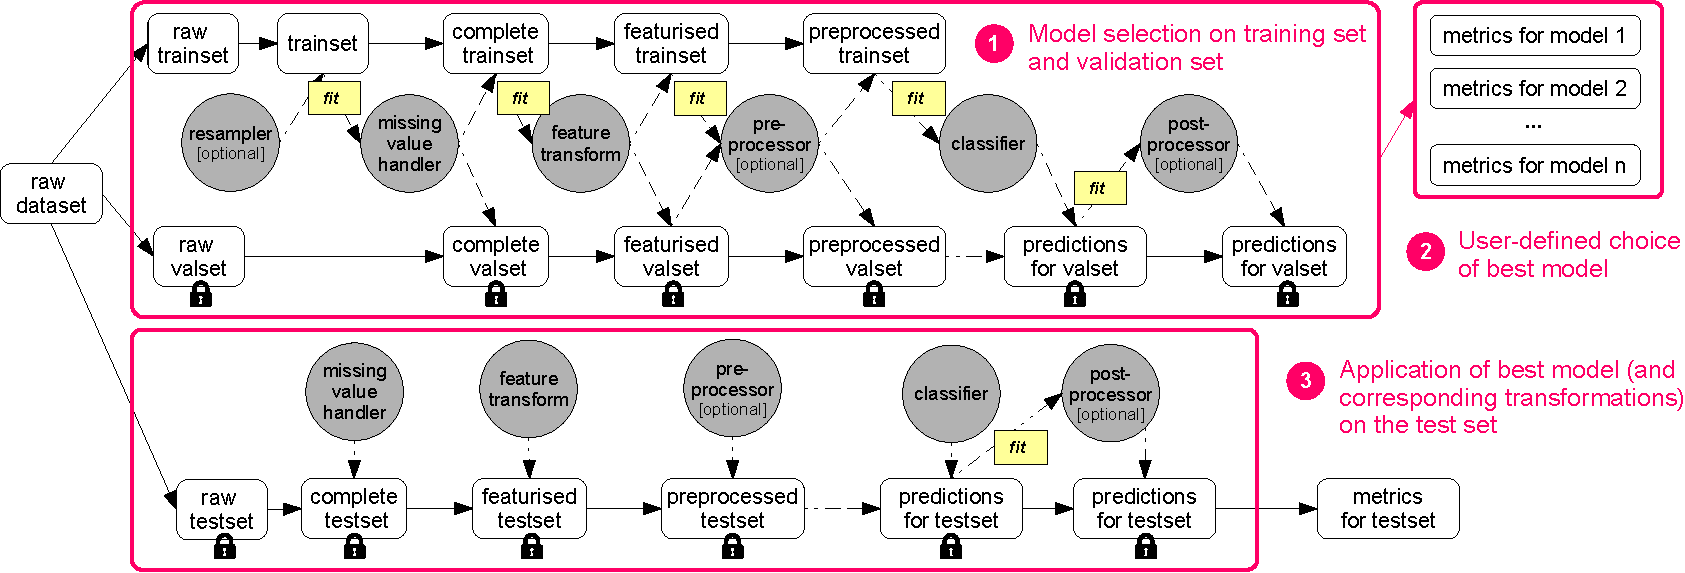
\includegraphics[scale=0.5]{figs/bigpicture-crop.pdf}  
  \caption{Data life cycle in \fairprep, designed to enforce isolation of  test data, and to allow for customization through user-provided implementations of different components. An evaluation run consists of three different phases: (1)~Learn different models, and their corresponding data transformations, on the training set; (2)~Compute performance / accuracy-related metrics of the model on the validation set, and allow the user to select the `best' model according to their setup; (3)~Compute predictions and metrics for the user-selected best model on the held-out test set.}
  \label{fig:bigpicture}
\end{figure*}

Figure~\ref{fig:bigpicture} summarizes the architecture of \fairprep, which is based on three main principles: 

\begin{enumerate}
\item Data isolation: to avoid target leakage, user code should only interact with the training set, and never be able to access the held-out test set. 

\item Componentization: different data transformations and learning operations should be implementable as single, exchangeable standalone components; the framework should expose simple interfaces to users, supporting low effort customization. 

\item Explicit modeling of the data lifecycle: the framework defines an explicit, standardized data lifecycle that applies a sequence of data transformations and model training in a predefined order. 
\end{enumerate}

\fairprep  currently focuses on data cleaning, including different methods for data imputation, and model selection and validation, including hyperparameter tuning, and can be extended to accommodate earlier lifecycle stages, such as data acquisition, integration, and curation.   Schelter~\etal~\cite{DBLP:conf/edbt/SchelterHKS20} measured the impact of sound best practices, such as hyperparameter tuning and feature scaling, on the fairness and accuracy of the resulting classifiers, and also showcased how \fairprep enables the inclusion of incomplete data into studies and helps analyze the effects.  

If Ann wants to ensure that she follows sound experimentation practices during model development, she can use the \fairprep library as a runtime platform for experiments, for example to compute various fairness related metrics for the predictions of her classifier. Furthermore, she can leverage the component architecture of \fairprep to evaluate different missing value imputation techniques and fairness enhancing interventions to see whether these help with mitigating the low accuracy that she encountered in her model for the predictions for middle-aged women, as discussed in our running example in Section~\ref{sec:intro}.

\header{Source code} A prototype implementation of FairPrep is available at \surl{https://github.com/DataResponsibly/FairPrep}.

% !TEX root = main.tex
\subsection{Detecting Data Distribution Bugs Introduced in Preprocessing}
\label{sec:mlinspect}

In our recent work on the \textit{mlinspect} library~\cite{grafberger2021mlinspect}, we focus on helping data scientists diagnose and mitigate problems to which we collectively refer as \emph{data distribution bugs}. These types of bugs are often introduced during preprocessing, for reasons we outlined in Section~\ref{sec:dim}.  For example, preprocessing operations that involve filters or joins can heavily change the distribution of different groups in the training data~\cite{fairdags}, and missing value imputation can also introduce skew~\cite{schelter2019fairprep}.  Recent ML fairness research, which mostly focuses on the use of learning algorithms on static datasets~\cite{DBLP:journals/cacm/ChouldechovaR20} is therefore insufficient, because it cannot address such technical bias originating from the data preparation stage. In addition, we should detect and mitigate such bias as close to its source as possible.

Unfortunately, such data distribution issues are difficult to catch. In part, this is because different pipeline steps are implemented using different libraries and abstractions, and the data representation often changes from relational data to matrices during data preparation. Further, preprocessing in the data science ecosystem~\cite{dataScienceLookingGlass} often combines relational operations on tabular data with  \textit{estimator/transformer pipelines},\footnote{\url{https://scikit-learn.org/stable/modules/compose.html}} a composable and nestable abstraction for combining operations on array data, which originates from \stt{scikit-learn}~\cite{Pedregosa2011} and has been adopted by popular libraries like \stt{SparkML}~\cite{meng2016mllib} and \stt{Tensorflow Transform}. In such cases, tracing problematic  featurised entries back to the pipeline's initial human-readable input is tedious work.  Finally, complex estimator/transformer pipelines are hard to inspect because they often result in nested function calls not obvious to the data scientist.

Due to time pressure in their day-to-day activities, most data scientists will not invest the necessary time and effort to manually instrument their code or insert logging statements for tracing as required by model management systems~\cite{Vartak2018,zaharia2018accelerating}.  This calls for the development of tools that support \emph{automated inspection of ML pipelines}, similar to the inspections used by modern IDEs to highlight potentially problematic parts of a program, such as the use of deprecated code or problematic library functions calls. Once data scientists are pointed to such issues, they can use data debuggers like \stt{Dagger}~\cite{maddendagger} to drill down into the specific intermediate pipeline outputs and explore the root cause of the issue. Furthermore, to be most beneficial, automated inspections need to work with code natively written with popular ML library abstractions. 

\header{Lightweight inspection with \mlinspect} To enable lightweight pipeline inspection, we designed and implemented \mlinspect~\cite{grafberger2021mlinspect}, a library that helps data scientists automatically detect data distribution issues in their ML pipelines, such as the accidental introduction of statistical bias, and provides linting for best practices. The \mlinspect library extracts logical query plans, modeled as directed acyclic graphs (DAGs) of preprocessing operators from ML pipelines that use  popular libraries like \pandas and \sklearn, and combine relational operations and estimator/transformer pipelines. These plans are then used to automatically instrument the code and trace the impact of operators on properties like the distribution of sensitive groups in the data. 

Importantly, \mlinspect implements a library-independent interface to propagate annotations such as the lineage of tuples across operators from different libraries, and introduces only constant overhead per tuple flowing through the DAG. Thereby, the library offers a general runtime for pipeline inspection, and allows us to integrate many issue detection techniques that previously required custom code, such as automated model validation on data slices~\cite{SliceFinder}, the identification of distortions with respect to protected group membership in the training data~\cite{fairdags}, or automated sanity checking for ML datasets~\cite{hynes2017data}.

\begin{figure*}[t!]
  \centering
  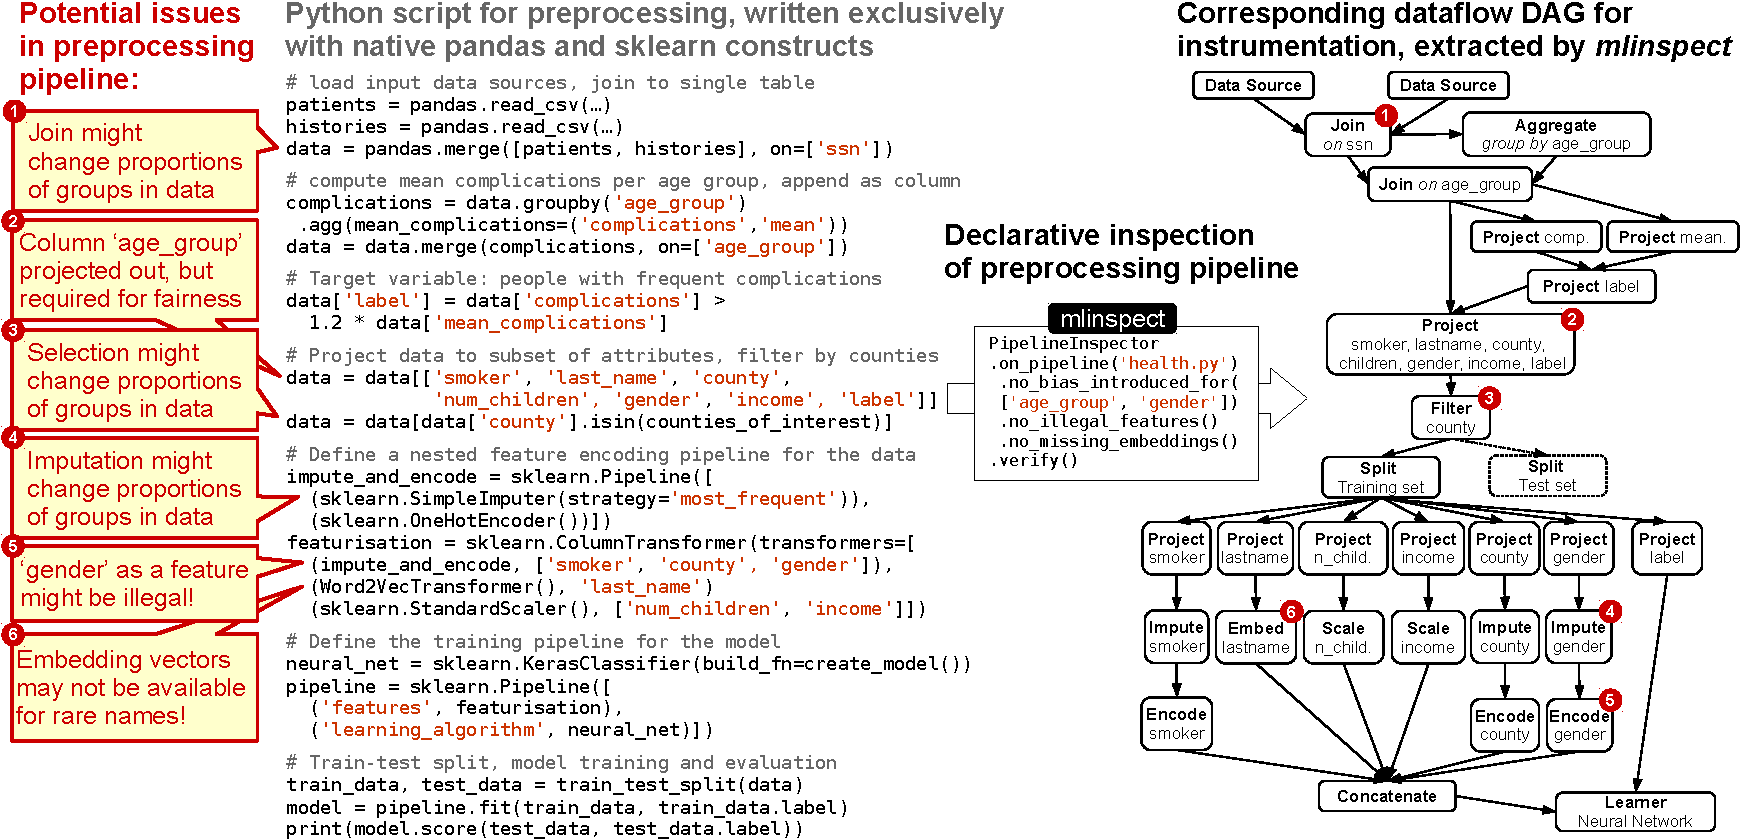
\includegraphics[width=\textwidth]{figs/example-crop.pdf}
  \caption{ML pipeline for our running example that predicts which patients are at a higher risk of serious complications, under the requirement to achieve comparable false negative rates across intersectional groups by gender and age group.  On the left, we highlight potential issues identified by \mlinspect. On the right, we show the corresponding dataflow graph, extracted to instrument the code and pinpoint the issues.}
  \label{fig:example}
\end{figure*}

\header{Identifying data distribution bugs in our running example} Figure~\ref{fig:example} shows a  preprocessing pipeline and potential data distribution bugs for our running example from Section~\ref{sec:intro}. The pipeline first reads two CSV files, which contain patient demographics and their clinical histories, respectively. Next, these dataframes are joined on the \stt{ssn} column. This join may introduce a data distribution bug (as indicated by issue \circled{1}) if a large percentage of the records of some combination of gender and age group do not have matching entries in the clinical history dataset. Next, the pipeline computes the average number of complications per age group and adds the binary target label to the dataset,  indicating which patients had a higher than average number of complications compared to their age group. The data is then projected to a subset of the attributes, to be used by the classification model. This leads to the second issue \circled{2} in the pipeline: the data scientist needs to ensure that the model achieves comparable accuracy across different age groups, but the age group attribute is projected out here, making it difficult to catch data distribution bugs later in the pipeline. The data scientist additionally filters the data to only contain records from patients within a given set of counties.  This may  lead to issue \circled{3}: a data distribution bug may be introduced if populations of different counties systematically differ in age.

Next, the pipeline creates a feature matrix from the dataset by applying common feature encoders with  \shref{https://scikit-learn.org/stable/modules/generated/sklearn.compose.ColumnTransformer.html}{\texttt{ColumnTransformer}} from \sklearn, before training a neural network on the features.   For the categorical attributes \stt{smoker}, \stt{county}, and \stt{gender}, the pipeline imputes missing values with mode imputation (using the most frequent attribute value), and subsequently creates one-hot-encoded vectors from the data. The \stt{last\_name} is replaced with a corresponding vector from a pretrained word embedding, and the numerical attributes \stt{num\_children} and \stt{income} are normalized. This feature encoding part of the pipeline introduces several potential issues: \circled{4} the imputation of missing values for the categorical attributes may introduce statistical bias, as it may associate records with a missing value in the gender attribute with the majority gender in the dataset; \circled{5} depending on the legal context (\ie if the disparate treatment doctrine is enforced), it may be forbidden to use \stt{gender}  as an input to the classifier; \circled{6} we may not have vectors for rare non-western names in the word embedding, which may in turn lead to lower model accuracy for such records. As illustrated by this example, preprocessing can give rise to subtle data distribution bugs that are difficult to identify manually, motivating the development of automatic inspection libraries such as \mlinspect, which will hint the data scientist towards these issues.

\header{Source code} A prototype implementation of \mlinspect, together with a computational notebook that shows how \mlinspect can be used to address the issues outlined in the ML pipeline in Figure~\ref{fig:example},  is available at \surl{https://github.com/stefan-grafberger/mlinspect}.


% !TEX root = main.tex
\subsection{Validating Serving Data with Data Unit Tests}
\label{sec:validate}

Machine learning (ML) techniques are very sensitive to their input data, as the deployed models rely on strong statistical assumptions about their inputs~\cite{sculley2015hidden}, and subtle errors introduced by changes in the data distribution can be hard to detect~\cite{polyzotis2017data}. At the same time, there is ample evidence that the volume of data available for training is often a decisive factor for a model’s performance~\cite{halevy2009unreasonable}.  How errors in the data affect performance, and fairness of deployed machine learning models is an open and pressing research question, especially in cases where the data describing protected groups has a higher likelihood of containing errors or missing values~\cite{DBLP:conf/edbt/SchelterHKS20}.

\header{Unit tests for data with \deequ} As discussed in Section~\ref{sec:bias-deployment}, accidental errors during data integration can heavily impact the prediction quality of downstream ML models. We therefore postulate that there is a pressing need for increased automation of data validation.   To respond to this need,
Schelter~\etal~\cite{schelter2018automating} presented \deequ, a data unit testing library. The library centers around the vision  that users should be able to write ‘unit-tests’ for data, analogous to established testing practices in software engineering, and is built on the following principles: 

\begin{enumerate}
    \item Declarativeness:  allowing data scientist to spend time on thinking about \emph{what} their data should look like, and not about \emph{how} to implement the quality checks.   \deequ offers a declarative API that allows users to define checks on their data by composing a variety of available constraints. 
    \item Flexibility: allowing users to leverage external data and custom code for validation (\eg call a REST service for some data and write a complex function that compares the result to some statistic computed on the data).  
    \item Continuous integration: explicitly supporting the incremental computation of quality metrics on growing datasets~\cite{schelter2019differential}, and allowing users to run anomaly detection algorithms on the resulting historical time series of quality metrics.
    \item Scalability: scaling seamlessly to large datasets, by translating the  data metrics computations to aggregation queries, which can be efficiently executed at scale with a distributed dataflow engine such as \stt{Apache Spark}~\cite{zaharia2012resilient}.
\end{enumerate}

\header{Unit testing serving data in our running example} A prime use case of \deequ in ML deployments is to test new data to be sent to the model for prediction. When Ann deploys her model for real world usage, she wants to make sure that it will only consume well-formed data. She can use \deequ to write down her assumptions about the data as a declarative data unit test, and have this test integrated into the pipeline that feeds data to the deployed model. If any  assumptions are violated, the pipeline will stop processing, the data will be quarantined, and a data engineer will be prompted to investigate the root cause of the failure.

Listing~\ref{lst:deequ} shows what  a data unit test may look like. We precompute certain expected statistics for the data such as the number patients to predict for, the valid age groups, and expected distributions by gender and age group. Next, we write down our assumptions about the data, similar to integrity constraints in relational databases. We declare the following checks: we assume that the size of the data corresponds to the expected number of patients, we expect social security numbers (the \stt{ssn} attribute) to be unique, and we expect no missing values for the \stt{lastname}, \stt{county}, and \stt{age\_group} attributes. We furthermore assume that the values of the \stt{smoker} attribute are Boolean, while in the \stt{num\_children} attribute comprises of integers, and we expect the \stt{age\_group} attribute to only contain valid age group values, as defined beforehand. We also expect values of the \stt{num\_children} attribute to be non-negative. Finally, we compare the distribution of age groups and gender in serving data to their expected distribution via the \stt{histogramSatisfies} constraint.  The user-defined function \stt{notDiverged} compares the categorical distributions of these columns and returns a Boolean value.

\begin{lstlisting}[style=myScalastyle, caption={Example of a data unit test.}, captionpos="b", label={lst:deequ}]
// Computed in advance
val expectedNumPatients = ...
val validAgeGroups = ...
val expectedGenderDist = ...
val expectedAgeGroupDist = ...

// Assumptions about data to predict on
val validationResultForTestData = VerificationSuite ()
  .onData(expectedNumPatients)
  .addCheck()
    .hasSize(numPatients)
    .isUnique("ssn")
    .isComplete("lastname", "county", "age_group")
    .hasDataType("smoker", Boolean)
    .hasDataType("num_children", Integral)
    .isNonNegative("num_children")    
    .isContainedIn("age_group", validAgeGroups)
    .histogramSatisfies("age_group", { ageGroupDist => 
      notDiverged(ageGroupDist, expectedAgeGroupDist) })
    .histogramSatisfies("gender", { genderDist => 
      notDiverged(genderDist, expectedGenderDist) })    
  .run()

if (validationResultForTestData.status != Success) {
  // Abort pipeline, notify data engineers
}
\end{lstlisting}

During the execution of the test, \deequ identifies the statistics required for evaluating the constraints and generates queries  in  \stt{SparkSQL} with  custom  designed  aggregation  functions to compute them. For performance reasons, it applies multi-query optimization to enable scan-sharing for the aggregation queries, minimizing the number of passes over the input data. Once the data statistics are computed, \deequ invokes the validation functions and returns the evaluation results to the user. 

\header{Source code} \deequ is available under an open source license at \surl{https://github.com/awslabs/deequ}. It for example forms the basis of Amazon's recent \stt{Model~Monitor} service\footnote{\tiny\url{https://aws.amazon.com/blogs/aws/amazon-sagemaker-model-monitor-fully-managed-automatic-monitoring-for-your-machine-learning-models/}} for concept drift detection in the \stt{SageMaker} machine learning platform.

% !TEX root = main.tex

\section{Conclusions and Future Research Directions}
\label{sec:conc}

In this paper we discussed dimensions of technical bias that can arise through the lifecycle of machine learning applications, both during model development and after deployment. We outlined several approaches to detect and mitigate such bias based on our recent work, and will now discuss promising directions for future research, where the data engineering community has the potential to make significant impact.  We see the overarching goal of this line of research not in mechanically scrubbing data or algorithms of bias, but rather in equipping  data scientists with tools that can help them identify technical bias, understand any trade-offs, and thoughtfully enact interventions.

\header{Integrating technical bias detection into general software development tooling} Data science is rapidly becoming an important part of the toolbox of a ``general software engineer'', and so methods for detection and mitigation of technical bias need to become part of that toolbox as well. The scope of these methods must be extended beyond binary classification, and they must embrace human-in-the-loop elements by providing visualisations and allowing end-users to control experiments with low effort. To achieve practical impact, it is important to integrate these methods into common computational notebooks such as Jupyter, and into general IDE's such as PyCharm.

\header{Automating data quality monitoring} The arising challenge of automating the operation of deployed ML applications is gaining a lot of attention recently, especially with respect to monitoring the quality of their input data~\cite{rukattowards}. As outlined in Sections~\ref{sec:dim} and~\ref{sec:fairprep}, data quality issues and the choice of a data cleaning technique can be a major source of technical bias. Existing approaches~\cite{baylor2017tfx,schelter2018automating} for this problem have not yet reached broad adoption, in part because they rely on substantial domain knowledge needed, for example, to define ``data unit tests'' and the corresponding similarity metrics, and to set thresholds for detecting data distribution shifts. Additionally, it is very challenging to test data during the earlier pipeline stages (\eg  data integration) without explicit knowledge of how an ML model will  transform this data at the later stages. 

We thus see a dire need for automated or semi-automated approaches to quantify and monitor data quality in ML pipelines. A promising direction is to treat historical data (for which no system failures were recorded and no negative user feedback has been received) as ``positive'' examples, and to explore anomaly detection-based methods to identify future data that heavily deviates from these examples. It is important to integrate a technical bias perspective into these approaches, for example, by measuring data quality separately for subsets of the data that correspond to historically disadvantaged or minority groups, since these groups tend to be more heavily hit by data quality issues~\cite{chung2019slice}.

\header{Integrating technical bias detection into continuous integration systems for ML} Continuous integration is an indispensable step of modern best practices in software engineering to control the quality of deployed software, typically by automatically ensuring that software changes pass a set of unit and integration tests before deployment. There is  ongoing work to adapt and reinvent continuous integration for the machine learning engineering process~\cite{renggli2019continuous}, which also exposes a lifecycle similar to the software engineering lifecycle, as discussed in Section~\ref{sec:dim}. We see the need to make detection techniques for technical bias, such as automated inspections and data unit tests, first-class citizen in ML-specific continuous integration systems.

\begin{thebibliography}{10}
  
\bibitem{Barocas2016}
Solon Barocas and Andrew~D. Selbst.
\newblock Big data's disparate impact.
\newblock {\em California Law Review}, 104(3):671--732, 2016.

\bibitem{baylor2017tfx}
Denis Baylor, Eric Breck, Heng-Tze Cheng, Noah Fiedel, Chuan~Yu Foo, Zakaria
  Haque, Salem Haykal, Mustafa Ispir, Vihan Jain, Levent Koc, et~al.
\newblock Tfx: A tensorflow-based production-scale machine learning platform.
\newblock In {\em Proceedings of the 23rd ACM SIGKDD International Conference
  on Knowledge Discovery and Data Mining}, pages 1387--1395, 2017.

\bibitem{Biessmann2018}
Felix Biessmann, David Salinas, Sebastian Schelter, Philipp Schmidt, and Dustin
  Lange.
\newblock Deep learning for missing value imputation in tables with
  non-numerical data.
\newblock In {\em Proceedings of the 27th ACM International Conference on
  Information and Knowledge Management}, pages 2017--2025. ACM, 2018.

\bibitem{DBLP:journals/corr/BowerKNSVV17}
Amanda Bower, Sarah~N. Kitchen, Laura Niss, Martin~J. Strauss, Alexander
  Vargas, and Suresh Venkatasubramanian.
\newblock Fair pipelines.
\newblock {\em CoRR}, abs/1707.00391, 2017.

\bibitem{DBLP:journals/cacm/ChouldechovaR20}
Alexandra Chouldechova and Aaron Roth.
\newblock A snapshot of the frontiers of fairness in machine learning.
\newblock {\em Commun. {ACM}}, 63(5):82--89, 2020.

\bibitem{chung2019slice}
Yeounoh Chung, Tim Kraska, Neoklis Polyzotis, Ki~Hyun Tae, and Steven~Euijong
  Whang.
\newblock Slice finder: Automated data slicing for model validation.
\newblock In {\em 2019 IEEE 35th International Conference on Data Engineering
  (ICDE)}, pages 1550--1553. IEEE, 2019.


\bibitem{DBLP:conf/forc/DworkIJ20}
Cynthia Dwork, Christina Ilvento, and Meena Jagadeesan.
\newblock Individual fairness in pipelines.
\newblock In Aaron Roth, editor, {\em 1st Symposium on Foundations of
  Responsible Computing, {FORC} 2020, June 1-3, 2020, Harvard University,
  Cambridge, MA, {USA} (virtual conference)}, volume 156 of {\em LIPIcs}, pages
  7:1--7:22. Schloss Dagstuhl - Leibniz-Zentrum f{\"{u}}r Informatik, 2020.

\bibitem{DBLP:journals/corr/FriedlerSV16}
Sorelle~A. Friedler, Carlos Scheidegger, and Suresh Venkatasubramanian.
\newblock On the (im)possibility of fairness.
\newblock {\em CoRR}, abs/1609.07236, 2016.

\bibitem{DBLP:journals/tois/FriedmanN96}
Batya Friedman and Helen Nissenbaum.
\newblock Bias in computer systems.
\newblock {\em {ACM} Trans. Inf. Syst.}, 14(3):330--347, 1996.

\bibitem{grafberger2021mlinspect}
Stefan Grafberger, Julia Stoyanovich, and Sebastian Schelter.
\newblock Lightweight inspection of data preprocessing in native machine
  learning pipelines.
\newblock In {\em CIDR}, 2021.

\bibitem{halevy2009unreasonable}
Alon Halevy, Peter Norvig, and Fernando Pereira.
\newblock The unreasonable effectiveness of data.
\newblock {\em IEEE Intelligent Systems}, 24(2):8--12, 2009.

\bibitem{DBLP:conf/fat/HeidariLGK19}
Hoda Heidari, Michele Loi, Krishna~P. Gummadi, and Andreas Krause.
\newblock A moral framework for understanding fair {ML} through economic models
  of equality of opportunity.
\newblock In {\em Proceedings of the Conference on Fairness, Accountability,
  and Transparency, FAT* 2019, Atlanta, GA, USA, January 29-31, 2019}, pages
  181--190. {ACM}, 2019.

\bibitem{hynes2017data}
Nick Hynes, D~Sculley, and Michael Terry.
\newblock The data linter: Lightweight, automated sanity checking for ml data
  sets.
\newblock {\em NIPS MLSys Workshop}, 2017.

\bibitem{kappelhof2017}
Joost Kappelhof.
\newblock {\em Total Survey Error in Practice}, chapter Survey Research and the
  Quality of Survey Data Among Ethnic Minorities.
\newblock 2017.

\bibitem{LehrOhm2017}
David Lehr and Paul Ohm.
\newblock Playing with the data: What legal scholars should learn about machine
  learning.
\newblock {\em UC Davis Law Review}, 51(2):653--717, 2017.

\bibitem{lipton2018detecting}
Zachary Lipton, Yu-Xiang Wang, and Alexander Smola.
\newblock Detecting and correcting for label shift with black box predictors.
\newblock In {\em International Conference on Machine Learning}, pages
  3122--3130, 2018.

\bibitem{maddendagger}
Samuel Madden, Mourad Ouzzani, Nan Tang, and Michael Stonebraker.
\newblock Dagger: A data (not code) debugger.
\newblock {\em CIDR}, 2020.

\bibitem{meng2016mllib}
Xiangrui Meng, Joseph Bradley, Burak Yavuz, Evan Sparks, Shivaram Venkataraman,
  Davies Liu, Jeremy Freeman, DB~Tsai, Manish Amde, Sean Owen, et~al.
\newblock Mllib: Machine learning in apache spark.
\newblock {\em JMLR}, 17(1):1235--1241, 2016.

\bibitem{Pedregosa2011}
Fabian Pedregosa, Ga\"{e}l Varoquaux, Alexandre Gramfort, et~al.
\newblock Scikit-learn: Machine learning in python.
\newblock {\em JMLR}, 12:2825--2830, 2011.

\bibitem{polyzotis2017data}
Neoklis Polyzotis, Sudip Roy, Steven~Euijong Whang, and Martin Zinkevich.
\newblock Data management challenges in production machine learning.
\newblock In {\em Proceedings of the 2017 ACM International Conference on
  Management of Data}, pages 1723--1726, 2017.

\bibitem{Polyzotis2018}
Neoklis Polyzotis, Sudip Roy, Steven~Euijong Whang, and Martin Zinkevich.
\newblock Data lifecycle challenges in production machine learning: A survey.
\newblock {\em SIGMOD Record}, 47:17--28, 2018.

\bibitem{SliceFinder}
Neoklis Polyzotis, Steven Whang, Tim~Klas Kraska, and Yeounoh Chung.
\newblock Slice finder: Automated data slicing for model validation.
\newblock {\em ICDE}, 2019.

\bibitem{dataScienceLookingGlass}
Fotis Psallidas, Yiwen Zhu, Bojan Karlas, et~al.
\newblock Data science through the looking glass and what we found there, 2019.

\bibitem{renggli2019continuous}
Cedric Renggli, Bojan Karlas, Bolin Ding, Feng Liu, Kevin Schawinski, Wentao
  Wu, and Ce~Zhang.
\newblock Continuous integration of machine learning models: A rigorous yet
  practical treatment.
\newblock {\em Proceedings of SysML 2019}, 2019.

\bibitem{rukattowards}
Tammo Rukat, Dustin Lange, Sebastian Schelter, and Felix Biessmann.
\newblock Towards automated ml model monitoring: Measure, improve and quantify
  data quality.
\newblock 2020.

\bibitem{Schelter2018c}
Sebastian Schelter, Felix Biessmann, Tim Januschowski, David Salinas, Stephan
  Seufert, Gyuri Szarvas, Manasi Vartak, Samuel Madden, Hui Miao, Amol
  Deshpande, et~al.
\newblock On challenges in machine learning model management.
\newblock {\em IEEE Data Eng. Bull.}, 41(4):5--15, 2018.

\bibitem{schelter2019differential}
Sebastian Schelter, Stefan Grafberger, Philipp Schmidt, Tammo Rukat, Mario
  Kiessling, Andrey Taptunov, Felix Biessmann, and Dustin Lange.
\newblock Differential data quality verification on partitioned data.
\newblock In {\em 2019 IEEE 35th International Conference on Data Engineering
  (ICDE)}, pages 1940--1945. IEEE, 2019.

\bibitem{schelter2019fairprep}
Sebastian Schelter, Yuxuan He, Jatin Khilnani, and Julia Stoyanovich.
\newblock Fairprep: Promoting data to a first-class citizen in studies on
  fairness-enhancing interventions.
\newblock {\em EDBT}, 2019.

\bibitem{DBLP:conf/edbt/SchelterHKS20}
Sebastian Schelter, Yuxuan He, Jatin Khilnani, and Julia Stoyanovich.
\newblock Fairprep: Promoting data to a first-class citizen in studies on
  fairness-enhancing interventions.
\newblock In Angela Bonifati, Yongluan Zhou, Marcos Antonio~Vaz Salles,
  Alexander B{\"{o}}hm, Dan Olteanu, George H.~L. Fletcher, Arijit Khan, and
  Bin Yang, editors, {\em EDBT}, pages 395--398. OpenProceedings.org, 2020.

\bibitem{schelter2018automating}
Sebastian Schelter, Dustin Lange, Philipp Schmidt, Meltem Celikel, Felix
  Biessmann, and Andreas Grafberger.
\newblock Automating large-scale data quality verification.
\newblock {\em Proceedings of the VLDB Endowment}, 11(12):1781--1794, 2018.

\bibitem{Sculley2015}
David Sculley, Gary Holt, Daniel Golovin, Eugene Davydov, Todd Phillips,
  Dietmar Ebner, Vinay Chaudhary, Michael Young, Jean-Francois Crespo, and Dan
  Dennison.
\newblock Hidden technical debt in machine learning systems.
\newblock In {\em Advances in neural information processing systems}, pages
  2503--2511, 2015.

\bibitem{sculley2015hidden}
David Sculley, Gary Holt, Daniel Golovin, Eugene Davydov, Todd Phillips,
  Dietmar Ebner, Vinay Chaudhary, Michael Young, Jean-Francois Crespo, and Dan
  Dennison.
\newblock Hidden technical debt in machine learning systems.
\newblock In {\em Advances in neural information processing systems}, pages
  2503--2511, 2015.

\bibitem{DBLP:journals/pvldb/StoyanovichHJ20}
Julia Stoyanovich, Bill Howe, and H.~V. Jagadish.
\newblock Responsible data management.
\newblock {\em Proc. {VLDB} Endow.}, 13(12):3474--3488, 2020.

\bibitem{Vartak2018}
Manasi Vartak and Samuel Madden.
\newblock Modeldb: Opportunities and challenges in managing machine learning
  models.
\newblock {\em IEEE Data Eng.}, 41:16--25, 2018.

\bibitem{fairdags}
Ke~Yang, Biao Huang, Julia Stoyanovich, and Sebastian Schelter.
\newblock Fairness-aware instrumentation of preprocessing pipelines for machine
  learning.
\newblock {\em HILDA workshop at SIGMOD}, 2020.

\bibitem{zaharia2018accelerating}
Matei Zaharia, Andrew Chen, Aaron Davidson, Ali Ghodsi, Sue~Ann Hong, Andy
  Konwinski, Siddharth Murching, Tomas Nykodym, Paul Ogilvie, Mani Parkhe,
  et~al.
\newblock Accelerating the machine learning lifecycle with mlflow.
\newblock {\em IEEE Data Eng. Bull.}, 41(4):39--45, 2018.

\bibitem{zaharia2012resilient}
Matei Zaharia, Mosharaf Chowdhury, Tathagata Das, Ankur Dave, Justin Ma, Murphy
  McCauly, Michael~J Franklin, Scott Shenker, and Ion Stoica.
\newblock Resilient distributed datasets: A fault-tolerant abstraction for
  in-memory cluster computing.
\newblock In {\em NSDI}, pages 15--28, 2012.

\end{thebibliography}
\end{document}

\end{article}
%
%\makeatletter
%\renewcommand{\AB@affillist}{}
%\renewcommand{\AB@authlist}{}
%\setcounter{authors}{0}
%\makeatother
%
\begin{article}
{Are Parity-Based Notions of AI Fairness Desirable?}
{James Foulds and Shimei Pan}
\graphicspath{{submissions/foulds_pan_final/}}
\documentclass[11pt,dvipdfm]{article}
%\documentclass[11pt]{article}
\usepackage{deauthor,times,graphicx,hyperref} 

\usepackage{amsmath, amssymb, amsfonts} %JF: removed amsthm which causes an error due to a duplicate definition

\def\BibTeX{{\rm B\kern-.05em{\sc i\kern-.025em b}\kern-.08em
    T\kern-.1667em\lower.7ex\hbox{E}\kern-.125emX}}


% \newtheorem{definition}{Definition}[section] %depending on the style file used, these lines may need to be commented out
% \newtheorem{theorem}{Theorem}[section]
% \newtheorem{corollary}{Corollary}[section]
% \newtheorem{lemma}{Lemma}[section]

%The following packages are used to make the causal assumptions figure, but are no longer needed since I saved the figure to a separate pdf.
%\usepackage{booktabs}
%\usepackage{tikz}
%\usetikzlibrary{bayesnet}

\usepackage{breakcites} %Fixes citations exceeding the margin!!

% \newtheorem{example}{Example} 
% \newtheorem{theorem}{Theorem}
% \newtheorem{lemma}[theorem]{Lemma} 
% \newtheorem{proposition}[theorem]{Proposition} 
\newtheorem{remark}[theorem]{Remark}
% \newtheorem{corollary}[theorem]{Corollary}
% \newtheorem{definition}[theorem]{Definition}
% \newtheorem{conjecture}[theorem]{Conjecture}
% \newtheorem{axiom}[theorem]{Axiom}
%%%
\newtheorem{dfn}[theorem]{Definition}

%\usepackage{todonotes}
%\newcommand{\jf}[1]{{\bf \color{orange}{jf: #1}}} %JF: commented out these TODO comment macros to make sure I didn't miss removing any.  Put them back if we ever edit this collaboratively again
%\newcommand{\shimei}[1]{{\bf \color{blue}{shimei: #1}}}
\setcounter{topnumber}{2}
\setcounter{bottomnumber}{2}
\setcounter{totalnumber}{4}
\renewcommand{\topfraction}{0.85}
\renewcommand{\bottomfraction}{0.85}
\renewcommand{\textfraction}{0.15}
\renewcommand{\floatpagefraction}{0.7}

% Definitions of handy macros can go here

\newcommand{\dataset}{{\cal D}}
\newcommand{\fracpartial}[2]{\frac{\partial #1}{\partial  #2}}

\begin{document}
\title{Are Parity-Based Notions of AI Fairness Desirable?}
\author{James R. Foulds and Shimei Pan\\ 
University of Maryland, Baltimore County\\ 
\{jfoulds, shimei\}@umbc.edu}


\maketitle
\begin{abstract}
It is now well understood that artificial intelligence and machine learning systems can potentially exhibit discriminatory behavior.  A variety of AI fairness definitions have been proposed which aim to quantify and mitigate bias and fairness issues in these systems.  Many of these AI fairness metrics aim to enforce parity in the behavior of an AI system between different demographic groups, yet parity-based metrics are often criticized for a variety of reasons spanning the philosophical to the practical.  The question remains: are parity-based metrics valid measures of AI fairness which help to ensure desirable behavior, and if so, when should they be used?  We aim to shed light on this question by considering the arguments both for and against parity-based fairness definitions.  Based on the discussion we argue that parity-based fairness metrics are reasonable measures of fairness which are beneficial to maintain in at least some contexts, and we provide a set of guidelines on their use.
\end{abstract}

\section{Introduction}
As artificial intelligence (AI) and machine learning (ML) systems are now widely deployed to automate decisions with substantial impact on human lives and our society including bail and sentencing decisions~\cite{angwin2016machine}, lending~\cite{applecard}, and hiring~\cite{dastin2018amazon}, these systems have come under increasing scrutiny.  According to the 2019 report from the AI Now Institute at New York University, ``\emph{tech companies are,
in fact, deeply aware that algorithmic discrimination is entrenched in the systems with which they are blanketing the world,}'' even if these companies have not always successfully addressed it~\cite{crawford2019ai}. In response to these concerns, a new and rapidly growing field of research on AI fairness has emerged which aims to study these issues and propose solutions.

To date, much of the research on AI fairness ---at least that which has arisen from the computer science community--- has centered around mathematical definitions or metrics which aim to quantify the degree of fairness or bias in an AI/ML system \cite{dwork2012fairness}.  We focus here on fairness in classification algorithms in which an individual's predicted class label is used to make a decision that directly impacts that individual.  For example, a prediction on whether an individual will repay a loan may determine whether that individual is offered a loan.  Thus, if the behavior of the system is unfair or discriminatory it may produce harm to the affected individuals and to the health of our society, due to perpetuating (or even exacerbating) discriminatory patterns in real-world outcomes which are reflected in the training data \cite{barocas2016big}.

Given the predictions made by a classification model, an AI fairness metric produces a score which assesses the extent that the model's behavior is fair or unfair (e.g. if it exhibits harmful behavior such as a bias toward or against a particular demographic group).  With a fairness metric in hand, the typical fair AI approach is to modify machine learning algorithms such that the training procedure penalizes solutions according to their degree of unfairness under the metric, or are constrained to produce a solution where the fairness metric is considered satisfactory \cite{dwork2012fairness}.  Hence, the ``fairness'' of an AI system is improved compared to the same system without this mitigation procedure, to the extent that the chosen metric successfully encodes what it means for the system to be ``fair.''  It is important to note that AI fairness is a complex sociotechnical problem which cannot be solved by the purely technical ``band-aid'' of enforcing a mathematical fairness definition without due consideration of non-technical factors \cite{crawford2019ai}.  Nevertheless, mathematical fairness definitions and learning algorithms that enforce them are valuable tools as part of a solution to unwanted discrimination in AI, which ideally would further consider sociotechnical, contextual, historical, legal, and stakeholder-centric perspectives in the design of the system.  

Many, perhaps even the majority, of proposed AI fairness metrics and fair learning algorithms aim to ensure that different protected demographic groups, e.g. along lines of gender, race, nationality, sexual orientation, age, social class, or political affiliation, are treated similarly overall by the algorithm.  For example, the metrics may enforce that the likelihood of being offered a loan, or being admitted to college, as determined by an AI algorithm, is approximately equal for men and women overall, or for other sensitive demographic groups.  The goal may be to ensure near-parity on the distribution of assigned class labels (i.e. \emph{outcomes} of the decision-making process) per group, as in the aforementioned example, or near-parity on error rates per group (e.g., false negative rates should be similar per demographic).  We refer to fairness metrics that encourage \emph{parity of class labels/outcomes} as \textbf{parity-based fairness metrics}.\footnote{While parity on error rates is clearly a type of fairness involving parity, the terms \emph{statistical parity} and \emph{demographic parity} usually refer to parity on outcomes in the AI fairness literature \cite{dwork2012fairness}.  Parity on error rates is also subject to substantially less criticism and controversy since improving it can be achieved by improving classification performance, so there is not an explicit accuracy-fairness trade-off \cite{hardt2016equality}. We therefore do not include it under the term ``\emph{parity-based}'' fairness in our discussion. }

%\shimei{There is also a notion of parity on treatment. Should we discuss it here?} \jf{Do you have a particular reference in mind? Do you mean threshold tests from the Stanford group, Goel and colleagues?}
%\shimei{I checked again. According to Zafar and colleagues, to ensure parity in treatment (or treatment parity), decision making systems need to avoid using users’ sensitive attribute information, i.e., avoid using the membership information in socially salient groups (e.g., gender, race), which are protected by anti-discrimination laws. Thus it is not really a parity-based fairness measure. It is more like a bias mitigation method (fairness through unawareness).} \jf{Got it. Some authors call this ``fairness through unawareness'' with reference to Dwork.  Corbett-Davies and Goel called it ``anti-classification.''}
%\jf{I added a section on disparate treatment / fairness through unawareness under non-parity based metrics.} 
Such parity-based metrics are intuitively appealing to many since they operationalize \textbf{equality}: \emph{each group is equally distributed outcomes (loans, college admissions, etc.) on average and no group is systematically favored or neglected by the procedure.}  Parity-based fairness metrics have however frequently been criticized in the literature \cite{dwork2012fairness, hardt2016equality, simoiu2017problem}.  Perhaps the most enduring critique is that parity-based fairness metrics do not necessarily ensure a \textbf{meritocracy}: \emph{it is possible that some ``deserving'' individuals or groups are not rewarded with favorable outcomes, and some ``undeserving'' individuals or groups might be rewarded with favorable outcomes} \cite{hardt2016equality, simoiu2017problem, corbettdavies2018measure}.  A number of alternative fairness definitions have been proposed, many of which aim to more concretely advance meritocratic ideals, generally at the expense of advancing equality relative to parity-based fairness.  Since societal processes are generally inequitable it is not usually possible to simultaneously achieve perfect equity and perfect meritocracy, so a choice must be made.  Whether to prioritize equality or meritocracy is a classic left-wing / right-wing political debate, so differing views on the value and validity of parity-based fairness are likely partially explained by differences in opinion along the left-right political spectrum.

On the other hand, many additional criticisms of parity-based fairness have been put forth, as we shall discuss in detail.  In the academic literature, the criticisms are usually placed when defending alternative fairness notions.  After all, if simple parity were enough to achieve fairness, how could we justify the existence of the field of fairness in AI as a deep and complex area of study?   Some authors (and skeptical peer-reviewers) have gone as far as to question its validity.  In a blog post, Hardt \cite{Hardt2016approaching} states:
\begin{quote}
    \emph{``To be sure, there is a set of applications for which demographic parity is not unreasonable, but this seems to be a subtle case to make. Any paper adopting demographic parity as a general measure of fairness is fundamentally flawed.''\cite{Hardt2016approaching}}
\end{quote}
Is Hardt right?  This raises some important questions.  \emph{Is the widespread practice of parity-based fairness a reasonable and useful approach, at least in some contexts?  Do its detractors have valid points that would preclude the use of parity-based fairness metrics by any reasonable scholar, regardless of political views and value systems?  In what cases should we use parity-based fairness metrics instead of alternatives?}

This paper aims to illuminate these questions by considering the main arguments and counterarguments on both sides of the issue.  We will ultimately conclude that parity-based fairness has its place, even if it is not always ideal, and we will provide guidelines on its use.
%The authors of this paper are not impartial to the debate, as we have proposed and applied parity-based fairness methods of our own, notably our \emph{differential fairness} metric (although we also provide alternative fairness definitions for the cases where parity-based fairness is not appropriate), but the arguments should be considered on their own merits.  

\subsection{Parity-Based Fairness Metrics}
To make the discussion concrete we begin by recalling the most well-known fairness metrics, beginning with parity-based approaches. For a more comprehensive summary of AI fairness metrics, we direct the reader to \cite{berk2017fairness} and \cite{20plusdefinitionssuervey}.  \emph{Readers from non-technical backgrounds should feel free to skip the mathematical details, which we include for precision but which are not essential to the discussion.}  We will use the following notation.  Suppose $\mathbf{x} \in \chi$ is an individual's data, $y \in Y$ is the class label for the corresponding individual, and $s \in A$ is a protected attribute corresponding to membership of one or more sensitive demographic groups.  A classifier $M(\mathbf{x})$ is a mechanism which takes an individual's data and makes a prediction $\hat{y}$ on their class. For example, the mechanism $M(\mathbf{x})$ could be a deep learning model for a lending decision, and $s$ could be the applicant's \emph{gender} and/or \emph{race}.  In many cases of interest, the predicted class label $\hat{y}$ corresponds to a \emph{decision that impacts the individual}.  For example, predicting that an individual will not repay a loan may correspond to a decision to deny that individual a loan.  We will therefore often refer to $\hat{y}$ as an \emph{outcome}. 

\noindent \textbf{The 80\% Rule and the $p$\% Rule:} The \emph{80\% rule}, a.k.a. the \emph{four-fifths rule}, is a legal guideline for identifying discrimination in the form of adverse or disparate impact in policies and practices on different protected groups, originally defined in the context of employment and personnel decisions \cite{eeoc1966guidelines}.  Disparate impact occurs when the same policies or procedures are applied to all individuals (e.g. in AI fairness, the same classifier is applied to everyone), but they impact different protected groups differently on average, even without explicit discrimination based on membership of the protected group.  The guidelines state:
\begin{quote}
\emph{
A selection rate for any race, sex, or ethnic group which is less than four-fifths (or 80\%) of the rate for the group with the highest rate will generally be regarded by the Federal enforcement agencies as evidence of adverse impact, while a greater than four-fifths rate will generally not be regarded by Federal enforcement agencies as evidence of adverse impact} \cite{eeoc1966guidelines}.
\end{quote}

Mathematically, the 80\% rule criterion identifies disparate impact in cases where
\begin{align}
%P(y=1|s_1)/P(y=1|s_2) \leq 0.8 \mbox{ ,}
\frac{P(M(\mathbf{x}) = 1| \mbox{group A})}{P(M(\mathbf{x}) = 1| \mbox{group B})} < 0.8 \mbox{ .} \label{eqn:pPercent}
\end{align}
for a favourable outcome $y=1$, %disadvantaged group $s_1$, and best performing group $s_2$ \cite{eeoc1966guidelines}.  
disadvantaged group $A$ and advantaged group $B$.  %  A similar scenario can occur in a machine learning classifier which does not observe the protected group membership attribute.  
The 80\% rule can be extended to a numeric measurement of the fairness of an algorithm or process, called the $p$\% rule, by dropping the use of a fixed threshold and simply reporting the ratio in Equation \ref{eqn:pPercent} \cite{zafar2015fairness}:
\begin{dfn} ($p$\% rule \cite{zafar2015fairness})
\begin{align}
    %p\%(M) = P(y=1|s_1)/P(y=1|s_2) \mbox{ .}
    p\%(M) = \frac{P(M(\mathbf{x}) = 1| \mbox{group A})}{P(M(\mathbf{x}) = 1| \mbox{group B})} \mbox{ .}
\end{align}
Here, if $p\%(M)$ is 1 then the demographic groups have an equal probability of being assigned the favorable outcome by the classification model $M$, and higher scores are better as they correspond to increased parity.
\end{dfn}

\noindent \textbf{Statistical Parity, a.k.a. Demographic Parity:}  \cite{dwork2012fairness} defined (and criticized, see below) the fairness notion of \emph{statistical parity}, a.k.a. \emph{demographic parity}, which requires that the probabilities of each outcome are approximately equal for each group, up to a tolerance level $\epsilon$. %$P(y|s_i) \approx P(y|s_j)$ for any outcome $y$ and pairs of protected attribute values $s_i$, $s_j$, allowing for a tolerance $\epsilon$ on the precise probabilities.  %Differential fairness is closely related as it  also aims to match probabilities of outcomes, but measures differences using ratios, and allows for multiple protected attributes.  The criticisms of \cite{dwork2012fairness} are mainly related to ways in which subgroups of the protected groups can be treated differently while maintaining demographic parity, which they call ``\emph{subset targeting},'' and which \cite{kearns2018preventing} term ``\emph{fairness gerrymandering}.''  Differential fairness explicitly protects the intersection of multiple protected attributes, which can be used to mitigate some of these abuses. 
\begin{dfn} (Statistical parity \cite{dwork2012fairness}) A mechanism $M(x)$ satisfies \emph{statistical parity} between demographic groups $A$ up to bias $\epsilon$ if
\begin{align}
    D_{tv}\big ( p(Y|s_i), p(Y|s_j) \big ) \leq \epsilon \ \ \ \ \forall (s_i,s_j) \in A \times A \mbox{ ,}
\end{align}
where $D_{tv}(p,q) = \frac{1}{2} \sum_{y \in Y}|p(y) - q(y)|$ is the total variation distance between distributions $p$ and $q$.
\end{dfn}
Here, a smaller value of $\epsilon$ corresponds to better fairness. Note that both $p$\% and statistical parity encourage probabilities of outcomes to be similar between groups, with similarity measured via ratios in $p$\% and via differences in statistical parity.  The $p$\% metric assumes a binary class label and focuses on similar probabilities for a single favorable outcome $y=1$ (which would automatically promote having similar probabilities for the other binary outcome which is one minus its probability), while statistical parity aims for similar probabilities for each of two or more possible outcomes. 

\noindent \textbf{Intersectional and Subgroup Fairness Metrics:} Fairness metrics have been developed which aim to ensure parity for the subgroups of the protected groups which occur at the intersection of those groups, e.g. Black women. Such definitions include differential fairness \cite{foulds2020intersectional} and subgroup fairness \cite{kearns2018preventing}.

\subsection{Non-Parity Based Fairness Metrics}
Numerous fairness metrics which do not focus on parity of outcomes have also been proposed, which typically are argued to satisfy desirable properties that parity-based fairness metrics and other competing definitions do not achieve.  While a complete discussion is beyond the scope of this paper, we consider the most well-known metrics which epitomize their corresponding category of fairness measures. 

\ \\
\noindent \textbf{Fairness Through Unawareness:}
One simple strategy to address unfairness is to simply remove the protected attributes from the classifier, i.e. $s$ is not included as a feature in $x$.  This approach, called \emph{fairness through unawareness} \cite{dwork2012fairness} or \emph{anti-classification} \cite{corbettdavies2018measure}, prevents \emph{disparate treatment} \cite{zafar2015fairness}, the use of different criteria for different protected groups, which could result in explicit discrimination based on an individual's protected category and could have legal implications, e.g. in employment contexts under Title VII.  It does not however prevent \emph{disparate impact} (i.e. disparities in the outcomes), since other attributes may be ``proxy variables'' which are correlated with the class label \cite{barocas2016big}.  For instance, zip code is frequently highly correlated with race in the United States due to historical segregation policies.  Fairness through unawareness is not itself a metric, since it does not produce a score, but its limitations motivate both parity-based fairness metrics and the metrics below. 


\ \\
\noindent \textbf{Equalized Odds and Equality of Opportunity:} Motivated by claimed limitations of demographic parity (discussed below), \cite{hardt2016equality} proposed to instead ensure that a classifier has equal error rates for each protected group.  This fairness definition, called \emph{equalized odds}, can loosely be understood as a notion of ``demographic parity for error rates instead of outcomes.''  Unlike demographic parity, equalized odds rewards accurate classification, and penalizes systems only performing well on the majority group.  %The true predictor is always acceptable, unlike for demographic parity.
%However, theoretical work has shown that equalized odds is typically incompatible with correctly calibrated probability estimates \cite{pleiss2017fairness}.  It is also a relatively weak notion of fairness from a civil rights perspective compared to demographic parity, as it does not ensure that outcomes are distributed equally. 
\cite{hardt2016equality} also propose a variant definition called \emph{equality of opportunity}, which relaxes equalized odds to only apply to a ``deserving'' outcome (i.e. $y$ = 1). 

\ \\
\noindent \textbf{Individual Fairness:}  The \emph{individual fairness} definition, due to \cite{dwork2012fairness}, mathematically enforces the principle that \emph{similar individuals should get similar outcomes} under a classification algorithm.  An advantage of this approach is that it preserves the privacy of the individuals, which can be important when the user of the classifications (the \emph{vendor}), e.g. a banking corporation, cannot be trusted to act in a fair manner.
%However, this is difficult to implement in practice as one must define ``similar'' in a fair way.  The individual fairness property also does not necessarily generalize beyond training set.

\ \\
\noindent \textbf{Causal Fairness:} Causal approaches to AI fairness metrics aim to use causal inference to ensure that protected attributes are not causes of predicted class labels, as opposed to merely being correlated with them.  For example, under the \emph{counterfactual fairness} definition \cite{kusner2017counterfactual}, intervening to change protected attributes $A$, while holding things which are not causally dependent on $A$ constant, will not change the predicted distribution of outcomes.  %While theoretically appealing, there are difficulties in implementing this in practice.  First, it requires an accurate causal model at the fine-grained individual level, while even obtaining a correct population-level causal model is generally very difficult.  To implement it, we must solve a challenging causal inference problem over unobserved variables, which generally requires approximate inference algorithms. (In the case of differential fairness, we advocate the use of Bayesian models which typically require approximate inference as well, although empirical distributions can be used if sufficient data is available.) Finally, to achieve counterfactual fairness, the predictions (usually) cannot make direct use of any descendant of $A$ in the causal model.  This generally precludes using \emph{any of the observed features} as inputs.

\ \\
\noindent \textbf{Threshold Tests:} \cite{simoiu2017problem} aim to measure discriminatory bias by modeling risk scores $r(x) = p(y=0|x)$ and latent thresholds which are used to classify based on the risk, and requiring algorithms or policies to threshold risk scores at the same points for different protected groups when determining outcomes.

% Describe parity-based notions of fairness, give examples:
% -demographic parity / statistical parity
% p\% rule
% differential fairness and subgroup fairness

%Considerations:
%Error rates vs outcomes - parity on which? They are incompatible


\section{Arguments for Parity-Based Fairness Metrics}
\label{sec:forParity}
We will next consider arguments from each side of the debate, beginning with arguments that support the use of parity-based fairness metrics.

\subsection{Equality as a Social Good}
While much ink has been spilled in the AI fairness literature regarding the limitations of parity-based fairness, relatively few authors have explicitly defended it, despite widespread use.   In the U.S. constitution, Thomas Jefferson famously wrote that it is self-evident that ``all men are created equal'' \cite{constitution}. Perhaps, like Jefferson, its proponents find the value of equality to be self-evident.  The most simple argument for parity-based fairness is often left unstated: equality is seen by many as having intrinsic value as a fair state of our society.  Equality is particularly ---but not exclusively--- prioritized by the political left, who advocate for policies such as affirmative action which aim to level the playing field for historically marginalized groups \cite{dionne2004americans}.  If this does not resonate with you, consider the following thought experiment.  You, a parent, have two similarly behaved children and one toy.  Would it be more fair to give the toy to the slightly better behaved child, or to ask them both to take turns and share the toy equally?  If only one child were given the toy, would the other child view the situation as fair?

In an AI context, to unpack the goals and impacts of parity-based fairness it is important to distinguish between the \emph{statistical task} of predicting an unknown class label $y$, such as whether an individual will repay a loan, and the \emph{economic task} of making a decision which impacts an individual based on the prediction $\hat{y}$, such as awarding a loan to that individual \cite{corbettdavies2018measure}.  The former is concerned only with accurate prediction, but in the name of equity the latter may arguably deviate from the labels, even when perfectly predicted \cite{foulds2020intersectional}.  Whenever the assignment of class labels corresponds to the allocation of resources (e.g. a limited number of admissions to a prestigious program of study), improving metrics regarding the parity of outcomes can help to reduce social or economic inequality.  The statistical/economic distinction is especially important when the class (\emph{repay loan}) is chosen merely as a convenient measurable proxy for a good decision (\emph{award loan}), even though making a good decision, which may involve further nuances than given by the proxy class label and/or population-level impacts such as fairness, is the true goal of the system.

\subsection{Mitigating Unfair Disparities and Negative Stereotypes}
Disparate behavior of an AI system is frequently caused by unfair occurrences, which can be mitigated by enforcing parity-based metrics. 

\subsubsection{Mitigating Societal Bias}
\label{sec:societalBias}
Inequality in society is often due to unfair societal processes \cite{crenshaw1989demarginalizing, collins2002black}. This impacts data, so it can be important to rectify the observed unfair inequality when performing algorithmic decision-making ~\cite{barocas2016big}.  If society is unfair, how do we fairly respond?  President Lyndon B. Johnson considered this problem in his commencement Address at Howard University in 1965, titled ``To Fulfill These Rights'' \cite{johnson1965remarks}.  %\footnote{\url{https://teachingamericanhistory.org/library/document/commencement-address-at-howard-university-to-fulfill-these-rights/}} 
\cite{dionne2004americans} summarizes President Johnson's remarks as follows:
\begin{quote}
\emph{``Imagine a hundred-yard dash in which one of the two runners has his legs shackled together. He has progressed ten yards, while the unshackled runner has gone fifty yards.
%can shorten by commenting the next line if needed
At that point the judges decide that the race is unfair. How do they rectify the situation? Do they merely remove the shackles and allow the race to proceed? Then they could say that “equal opportunity” now prevailed. But one of the runners would still be forty yards ahead of the other. 
%[\ldots] 
Would it not be the better part of justice to allow the previously shackled runner to make up the forty-yard gap, or to start the race all over again? That would be affirmative action toward equality.''} \cite{dionne2004americans}, paraphrasing \cite{johnson1965remarks}.
%\cite{lbj1965}
\end{quote}
%Actual quote from LBJ1965:
%You do not take a person who, for years, has been hobbled by chains and liberate him, bring him up to the starting line of a race and then say, “you are free to compete with all the others,” and still justly believe that you have been completely fair.

%\shimei{One counter argument with regard to President Johnson's metaphor is its reliance on stereotypes and generalizations as there are many privileged black people and poor white people. What would be our response?} \jf{The quote doesn't specifically reference Black people, and applies generally to those who are unfairly disadvantaged, including women, the elderly, people with disabilities, etc.  Is there still an issue? The answer, if we need to state it, is that unfairness is intersectional over race, social class, etc.  Intersectionality considers that wealthy black women have different disadvantages to poor white men.}

%\shimei{I added the comment here because when I tried to search for the reference for lbj65, I saw these types of arguments frequently associated with the shackled runner metaphor.  Should we move this to the section on arguments against parity-based measure?  Even in the context of intersectionality,  people may argue that it is still a generalization as there will still be individual differences in each intersectional group e.g. privileged black women from Africa and poor white man from the U.S. What would be our responses?} \jf{I also just saw some of these responses in social media posts when looking for the proper citation. \cite{dionne2004americans}, who it appears paraphrased Johnson's remark as above (not a direct quote), describes the white working class backlash to affirmative action, which is very prescient regarding the current political moment and Trump supporters' views.  I believe these comments are about affirmative action and liberal politics in general, the metaphor being a representative of this.  So it would be better to address it later in the paper.  Intersectionality covers all intersections of disadvantage, so the theory in principle covers privileged Black women from Africa and poor white men from the US (even if conservatives don't see it that way, and may be frustrated with being left behind by liberal politics). }
%\jf{I added Section \ref{sec:affirmativeAct} to raise this issue, and I added a paragraph to address it in Section \ref{sec:responseAbuses} }

In President Johnson's metaphor, the shackles are of course a metaphor for unfair societal disadvantages.  In the humanities and legal literature, such unfair processes have been studied under the framework of \emph{intersectionality}.  % a lens for examining societal unfairness which originally arose from the observation that sexism and racism have intertwined effects, in that the harm done to Black women by these two phenomena is more than the sum of the parts  \citep{crenshaw1989demarginalizing,truth1851aint}.  The notion of intersectionality was later extended to include overlapping injustices along more general axes \citep{collins2002black}.
The term intersectionality was introduced by  Kimberl\'e Crenshaw in the 1980's \cite{crenshaw1989demarginalizing} and popularized in the 1990's, e.g. by Patricia Hill Collins \cite{collins2002black}, although the ideas are much older \cite{collective1977black,truth1851aint}.  
In its general form, intersectionality emphasizes that \emph{systems of oppression} built into society lead to \emph{systematic disadvantages along intersecting dimensions}, which include not only gender, but also race, nationality, sexual orientation, disability status, and socioeconomic class \cite{collective1977black,collins2002black,crenshaw1989demarginalizing,hooks1981ain,lorde1984age,truth1851aint}.  
%These systems are interlocking in their effects on individuals at \emph{each intersection of the affected dimensions}.  %\citep{collective1977black,crenshaw1989demarginalizing}.
%
%Systems of oppression can lead individuals to perform below their potential, for instance by reducing available cognitive bandwidth \citep{verschelden2017bandwidth}, or by increasing the probability of incarceration \citep{davis2011prisons,alexander2012new}.  
Examples of systems of oppression include racism, sexism, the prison-industrial complex, mass incarceration, and the school-to-prison pipeline \cite{davis2011prisons,alexander2012new}.   
In the context of AI and fairness, intersectionality has been considered by e.g. \cite{buolamwini2018gender,noble2018algorithms, foulds2020intersectional, foulds2020bayesian}.  
%\citep{buolamwini2018gender}, who studied the impact of the intersection of gender and skin color on computer vision performance, and by \citep{kearns2018preventing,hebert-johnson2018multicalibration}, who aimed to protect certain subgroups in order to prevent ``fairness gerrymandering.'' From a humanities perspective, \citep{noble2018algorithms} critiqued the behavior of Google search with an intersectional lens, by examining the search results for terms relating to women, people of color, and their intersections, e.g.  ``Black girls.''
%

As an example of a scenario affected by unfair processes, consider the task of predicting prospective students' academic performance for use in college admissions decisions.  As discussed in detail by \cite{verschelden2017bandwidth}, and references therein, individuals belonging to marginalized and non-majority groups are disproportionately impacted by challenges of poverty and racism (in its structural, overt, and covert forms), including chronic stress, access to healthcare, under-treatment of mental illness, micro-aggressions, stereotype threat, disidentification with academics, and belongingness uncertainty.  Similarly, LGBT and especially transgender, non-binary, and gender non-conforming students disproportionately suffer bullying, discrimination, self-harm, and the burden of concealing their identities.
These challenges are often further magnified at the intersection of affected groups.  A survey of 6,450 transgender and gender non-conforming individuals found that the most serious discrimination was experienced by people of color, especially Black respondents \cite{grant2011injustice}.
Verschelden explains the impact of these challenges as a tax on the ``cognitive bandwidth'' of non-majority students, which in turn affects their academic performance.  She states that the evidence is clear %She states:
\begin{quote}
	\emph{%The evidence is clear
	``...that racism (and classism, homophobia, etc.) has made people physically, mentally, and spiritually ill and dampened their chance at a fair shot at higher education (and at life and living).''} \cite{verschelden2017bandwidth}
\end{quote}
A classifier trained to predict students' academic performance from historical data hence aims to emulate outcomes that were substantially affected by unfair factors \cite{barocas2016big}.
An \emph{accurate predictor} for a student's GPA may therefore not correspond to a \emph{fair decision-making procedure} for student admissions.

\subsubsection{Mitigating Bias from Subjective Annotation}
Classification algorithms require labeled data to train on, and in many applications we must acquire labels through human annotation, which is often subjective, imperfect, and subject to the prejudice of the annotators \cite{barocas2016big}.  Consider for example the challenges of annotating whether a resume is a good match with a job ad \cite{ketki}, whether a prospective employee should be hired \cite{dastin2018amazon}, what emotion is being expressed in an image of a person's face \cite{barrett2019emotional}, whether a social media post is offensive \cite{HateSpeechDetectionBias}, whether an incarcerated individual is at high risk of committing another crime \cite{angwin2016machine}, or whether a prospective student should be admitted to a program of study \cite{lowry1988blot}.  In these scenarios the answers are not clear-cut, and so implicit bias can potentially impact the labeling process which determines the ``ground truth'' that the model aims to predict.  An extreme case occurred for the latter example when St George's Medical Hospital developed a computer program for initial screening of applicants to the school in the late 1970's to early 1980s.  The system aimed to replicate the decision-making processes of the selection panel, and was adjusted until it had more than 90\% correlation with the panel's scores.  In imitating the panel's behavior, the system was purposely designed to reduce the chance of an interview for candidates who were women or racial minorities 
\cite{lowry1988blot}.  While the potential for annotation bias does not imply that perfect parity of outcomes must be sought, it illustrates how unfair disparities can arise in the training data, which in turn suggests that methods which improve parity-based fairness metrics may be valuable tools for combating these unfair disparities.

%\subsection{Regularization, prevent bias amplification}
\subsubsection{Mitigating Harms of Representation}
In addition to causing economic and financial harm, AI systems that exhibit biased behavior may encode negative stereotypes, which can be hurtful, offensive, or reinforce low self-esteem in historically marginalized groups, as well as reinforcing prejudice against those groups.  For example, \cite{noble2018algorithms} studied how Google search results reflect negative stereotypes.  She discussed how searching for keywords related to marginalized groups such as ``Black girls'' returned mainly pornographic results, thereby perpetuating racist, sexist, and dehumanizing stereotypes.  Similarly, searching for ``three black teenagers'' returned mugshots, insinuating criminality, while searching for ``three white teenagers'' returned wholesome images.    Noble states:
\begin{quote}
    \emph{``What we need to ask is why and how we get these stereotypes in the first place and what the attendant consequences of racial and gender stereotyping do in terms of public harm for people who are the targets of such misrepresentation. \cite{noble2018algorithms}''}
\end{quote}
Such \emph{harms of representation} arise when the behavior of an AI system appears to attribute lower value or negative properties to groups or individuals.  This is especially hurtful when the misrepresentation due to the AI corresponds to the perpetuation of hateful views that are currently or historically advanced in racist, sexist, ableist, anti-semitic or other discriminatory language with deliberately hurtful intent \cite{noble2018algorithms}.  Harms of representation are problematic even when the outcomes of the AI system are not themselves consequential (e.g. if their consequences were limited to within a video game).  Similarly, in our own research we found that an AI-based career counseling system trained on social media data disproportionately recommends careers in computer science and executive/managerial positions to boys and homemaking, nursing, and customer service to girls \cite{islam2020neural}.  This behavior perpetuates stereotypes that could impact young people's perceptions of their own capabilities and potential when given recommendations by the algorithm.  We applied a parity-based fairness intervention which reduced the extent to which the system's results reflected gender stereotypes, addressing the harmful portrayal of gender groups by the algorithm, not to mention the potential financial impacts due to directing women toward less lucrative careers. 

\subsection{Practical Benefits}
Beyond mitigating unfair disparities and negative stereotypes, improving parity in AI systems has additional practical benefits that pertain to broad classes of applications, including the advantages of diversity and reduction of potential legal liability.

\subsubsection{Increasing Diversity}
In many AI applications a classification algorithm selects or impacts the set of individuals to be (potentially) included in an organization or program, e.g. in automated hiring decisions, college admissions, allocation of healthcare resources such as Medicaid services, and career recommendation (which could impact career choices).  In these scenarios, improving parity-based fairness metrics corresponds to an increase in the diversity of the pool of selected individuals in terms of the representation of the protected groups, which is generally accomplished by increasing the participation of underrepresented groups who have been historically marginalized.  Diversity is a crucial first step toward \emph{inclusion}, in which an organization maintains a culture in which members of diverse groups are given respect, fair treatment, and a voice in decision-making processes \cite{bell2011voice}. 

As well as the intrinsic and ethical importance of diversity and inclusion, diversity can potentially lead to improvement in organizational effectiveness and competitiveness \cite{page2008difference} including impacts on cost, resource acquisition, marketing, creativity, problem solving, and system flexibility \cite{cox1991managing}.  Standpoint theory, which emphasizes the shared experiences of members of historically marginalized groups such as women, Black women, and the working class, suggests that the different perspectives and \emph{situated knowledge} of members of historically marginalized groups as \emph{outsiders-within} an institution or organization controlled by the dominant group allow them to critique it in a way that the dominant group cannot \cite{hartsock1983feminist, collins2002black}.  Hence, increased representation of historically marginalized groups within an organization can potentially help it to break free from stagnant thought patterns and groupthink.  Diversity can also potentially lead to benefits to the economy.  A brief from the Economics and Statistics Administration in the U.S. Department of Commerce argues that a lack of gender diversity in STEM is a missed opportunity to expand STEM employment and thereby increase the nation's innovative capacity and global competitiveness, as well as reducing the gender wage-gap \cite{beede2011women}.

\subsubsection{Reducing Legal Liability}
The 80\% rule \cite{eeoc1966guidelines} is used as a legal criterion for demonstrating disparate impact under several anti-discrimination laws in the United States primarily regarding employment decisions, including Title VII of the Civil Rights Act of 1964, the Americans with Disabilities Act (ADA), and the Age Discrimination in Employment Act.  For example, Title VII prohibits employment discrimination on the basis of race, color, religion, sex, or national origin.  A finding of adverse impact under the criterion shifts the burden of proof to the organization to defend its employment practices against alleged discrimination.  %Title VII (prohibits employment discrimination) and Title IX (prohibits educational opportunities discrimination) of the Civil Rights Act of 1964, the Americans with Disabilities Act (ADA), and the Fair Housing Act (FHA). \textbf{TODO vERIFY THIS!!}
Leaving aside philosophical debate on what it means to be ``fair,'' ensuring a sufficient degree of parity may be important to avoid legal liability under these laws, providing a practical motivation for parity-based fairness interventions in AI systems in the context of any employment decision such as hiring or promotion. The disparate impact legal criterion potentially also extends to other spheres such as housing under the Fair Housing Act of 1968. 

\subsection{Summary} Parity-based fairness metrics aim to operationalize and measure the degree of \emph{equality} in the assignment of potentially consequential outcomes to protected groups.  Equality has intrinsic value as a desirable property for a fair and healthy society.  Unfair disparities and harmful stereotypes encoded in data used to train machine learning algorithms frequently arise from unfair processes, both in society and during data preparation, and parity-based fairness interventions can help mitigate them.  Ensuring parity-based fairness has additional practical benefits across a broad range of use cases including increasing diversity and avoiding legal liability for organizations. 

\section{Arguments Against Parity-Based Notions of Fairness}
\label{sec:againstParity}

%\shimei{In this section, we don't really need to counter-argue these arguments. We just need to describe them, right? In the next section (sec. 4), we can argue about the validity of these claims/arguments and then make recommendations on when parity-based measures are appropriate. }
%\jf{Ok, I will organize it that way}

The arguments from the previous section support the view that improving parity-based fairness is beneficial in many contexts, all other things being equal.  A number of criticisms have been put forth as well.  Some of the criticisms relate to what parity \emph{does}, i.e. potential harmful effects, and others relate to what parity \emph{does not do} which we might otherwise desire in a fairness metric. We discuss these concerns below.

%\subsection{Unreasonable Implicit Reasons Why Some Scholars and Practitioners Oppose Parity}
%Academic rat race and peer review process motivates solutions to be technically complex.  Authors are motivated to defend novel metrics, hence they criticize previous metrics including parity-based metrics. Explicit bias - cf. Lowry

\subsection{Parity Potentially Harms Accuracy / Utility}
A common criticism of parity-based fairness is that since the true class label distribution may not satisfy parity, ensuring parity would typically require a mismatch between the predictions and the data which would harm the prediction accuracy, and hence the economic utility of the system.  Example quotes from the literature include:\footnote{For presentation purposes, when quotes start mid-sentence we have modified them to capitalize the first letter.}
\begin{quote}
 \emph{``Demographic parity often cripples the utility that we might hope to achieve, especially in the common scenario in which an outcome to be predicated, e.g. whether the loan be will defaulted, is correlated with the protected attribute.''} \cite{hardt2016equality}
\end{quote}

\begin{quote}
\emph{``These mechanisms pay a significant cost in terms of the accuracy (or utility) of their predictions. In fact, there exist some inherent tradeoffs (both theoretical and empirical) between achieving high prediction accuracy and satisfying treatment and / or impact parity.''} \cite{zafar2017parity}
\end{quote}

\begin{quote}
\emph{``The thresholds required to optimally satisfy these classification parity constraints will typically differ from the optimal thresholds for any community. Thus, requiring classification parity (or even approximate parity) can hurt majority and minority groups alike.} \cite{corbettdavies2018measure}
\end{quote}


\subsection{Parity Does not Ensure a Meritocracy}
The goal of parity-based fairness is to uphold the ideal of \emph{equality}, in terms of the assignment of outcomes across protected groups.  It does not explicitly aim to uphold a competing ideal of fairness, \emph{meritocracy}, in which the ``most deserving'' individuals are assigned the greatest rewards, although mitigating discrimination and unfair disadvantages could perhaps be considered meritocratic \cite{johnson1965remarks}.  Some authors have further argued that enforcing parity can be in conflict with the goal of a meritocracy.
\subsubsection{Infra-Marginality}
Arguments against parity-based fairness via the concept of \emph{infra-marginality} are emblematic of a meritocratic-centered view on fairness in AI and elsewhere.  The term was coined by \cite{ayres2002outcome} in the context of detecting discrimination in police practices, and was considered in the context of AI fairness by \cite{corbettdavies2018measure} and implemented in a statistical modeling approach by \cite{simoiu2017problem}.  This view of fairness adopts a framework in which features $x$ determine idealized risk scores $r(x) = P(y=0|x)$ which correspond to the probability that an individual has a negative class label, e.g. they will commit a crime in future (or alternatively, ``qualification'' or ``merit'' scores corresponding to the probability of a positive label $y=1$ such as graduating from a particular university).  It is assumed that risk scores encapsulate how ``(un)deserving,'' ``(un)qualified'' or ``(in)capable'' an individual is.  Hence, estimated risk scores $s(x)$ are ideally thresholded in order to assign beneficial labels to more ``qualified'' individuals, or detrimental outcomes to more ``risky'' individuals.  Classifying via a fixed risk threshold (regardless of demographic group) would correspond to some notion of equal treatment, hence avoiding disparate treatment or (it is argued) \emph{unjust} disparate impact, although ``justified'' disparate impact (i.e. ``justified'' disparities in outcomes between groups) may still occur \cite{corbettdavies2018measure}.   Such a classifier would implement a kind of meritocracy, since classifications are made based on solely on risk which is meant to correspond to a measure of deservedness of a particular outcome.

The term ``\emph{infra-marginal}'' means ``away from the threshold'' and usually refers to averages over risk scores for a particular demographic, e.g. average outcome probabilities or error rates.  According to \cite{corbettdavies2018measure,simoiu2017problem}, the ``\emph{inframarginality problem}'' with statistical tests for discrimination or AI bias that are computed based on per-demographic averages is that since the distribution of $x$ differs per demographic, the distribution of (idealized, ground-truth) risk scores $r(x)$ will typically also differ.  Hence, differences in the quantities used to compute parity-based fairness metrics and other similar fairness metrics,  which are calculated based on averages over risk scores, including ground-truth outcome probabilities $P(y|s)$, predicted outcome probabilities $P(M(x)|s)$ or error rates $P(M(x)|s,y)$, are expected to differ per group.  According to \cite{corbettdavies2018measure} and \cite{simoiu2017problem}, 
\begin{quote}
    \emph{``It is hard to determine whether differences in error rates are due to discrimination or to differences in the risk distributions.''} \cite{corbettdavies2018measure}
\end{quote}
\begin{quote}
\emph{``Even absent discrimination, the repayment rates for minority and white loan recipients might differ if the two groups have different risk distributions.''} \cite{simoiu2017problem}
\end{quote}
If a disparity in outcome probabilities is due to a different distribution in risk between demographics, presumed fair, legitimate, and well estimated, reducing the disparity via a fairness intervention would give an unearned advantage or disadvantage to members of different groups, making the system's behavior less meritocratic. 

%Moreover,  parity-based fairness metrics may not have a direct correspondence with differences in the classification threshold per demographic, which is assumed to be the definition of discrimination by  \cite{corbettdavies2018measure, simoiu2017problem} (e.g. thresholding males at a risk score of 5\% and and females at a risk score of 15\%).

%Many fairness definitions aim (implicitly or otherwise) to uphold the principle of \textbf{infra-marginality}, which states that differences between protected groups in the distributions of ``merit'' or ``risk'' (e.g. the probability of criminal recidivism) should be taken into account when determining whether bias has occurred \cite{simoiu2017problem}.



%A closely related argument is that parity of outcomes between groups is at odds with accuracy \citep{dwork2012fairness,hardt2016equality}.  




\subsubsection{Disparities can be Due to Confounding}
\emph{Confounding variables}, which are extraneous variables that impact the relationship between two variables such as protected demographic groups and outcomes, are another possible source of disparity other than discrimination.  This possibility motivates the use of causal inference methods to determine unfair bias \cite{kusner2017counterfactual, nabi2018fair}.  
\begin{quote}
    \emph{Any approach that relies on associative measures of [discrimination] will be led astray due to failing to properly model sources of confounding for the relationship of the sensitive feature and the outcome. }\cite{nabi2018fair}
\end{quote}
In a classic real-world case of confounding in measuring discrimination studied by \cite{bickel1975sex}, UC Berkeley's graduate admissions process admitted men at a higher rate than women in the Fall 1973 quarter.  On closer examination, it was found that more than half of the departments admitted women at a higher rate than men.  This apparent paradox, an instance of a phenomenon called Simpson's paradox, is explained by the fact that women were more likely to apply to more selective departments.  In this case, the choice of department to apply to is the confounding variable.  Since the disparity in admissions was caused by confounding rather than discriminatory bias, a parity-based fairness intervention might introduce a new bias that makes the procedure less meritocratic than the status quo due to giving an unmerited advantage to one demographic.

\subsection{Parity does not Prevent Certain Harms or Abuses, or Provide Certain Benefits}
There are many possible desiderata for fairness, such as preventing certain conceivable harms or conferring certain benefits, which parity-based fairness does not accomplish. Naturally, this is also true of any other possible fairness metric.  Here we give several of the most well-known examples. 
\subsubsection{Subset Targeting, a.k.a. Fairness Gerrymandering}
Parity-based fairness metrics only protect parity for the groups that are defined, and not subgroups within them.  Subgroup targeting, also known as fairness gerrymandering, occurs when subgroups of a protected group are treated in an unfair way while preserving parity for the top-level groups \cite{dwork2012fairness,kearns2018preventing}. 
\begin{quote}
    \emph{Imagine a setting with two binary features,
corresponding to race (say black and white) and gender (say male and female), both of which are distributed independently and uniformly at random in a population. Consider a classifier that labels an example positive if and only if it corresponds to a black man, or a white woman. Then the classifier will appear to be equitable when one considers either protected attribute alone, in the sense that it labels
both men and women as positive 50\% of the time, and labels both black and white individuals as positive 50\% of the time. But if one looks at any conjunction of the two attributes (such as black women), then it is apparent that the classifier maximally violates the statistical parity fairness constraint.}  \cite{kearns2018preventing} 
\end{quote}



% \subsection{"How can a perfectly accurate classifier be biased?"}
%   cf Moritz Hardt blog post

% \subsection{Does not always admit a perfectly accurate classifier}
%  cf Moritz Hardt Equality of Opportunity

% \subsection{Fairness definitions are incompatible with each other}
%  - Berk


%\subsubsection{Parity Does not Correct for Past Injustices}
%(only prevents new injustices)

\subsubsection{Tokenism and the Self-Fulfilling Prophecy}

Parity-based fairness leaves a lot of leeway on the nature of the chosen solution, which could potentially be abused by a malicious actor.  The potential for deliberate harm is even greater when one considers the broader socio-technical setting in which the AI system resides.  For example, it is easy to construct scenarios in which parity is satisfied by a classifier that behaves in a highly unmeritocratic way: 
\begin{quote}
\emph{``The notion permits that we accept the qualified applicants in one demographic, but random individuals in another, so long as the percentages of acceptance match. This behavior can arise naturally, when there is little or no training data available for one of the demographics.''} \cite{hardt2016equality}
\end{quote}
This scenario is essentially \emph{tokenism}, the selection of unqualified members of under-represented groups as lip-service to diversity and inclusion, which creates its own problems \cite{weisskopf2004affirmative}, such as the following:
\begin{quote}
    \emph{``Because demographic parity leads to affirmative action, it leads to recurrent criticism. Such criticism can contribute to undermining the reputation of the minority group in the long term.''} \cite{Landeau2020}
\end{quote}

\cite{dwork2012fairness} identify a related and even more harmful potential abuse which they call the \emph{self-fulfilling prophecy}. 
\begin{quote}
\emph{``This is when unqualified members of [protected group] $S$ are chosen, in order to justify future discrimination against $S$ (building a case that there is no point in ``wasting'' resources on $S$). Although senseless, this is an example of something pernicious that is not ruled out by statistical parity, showing the weakness of this notion.''} \cite{dwork2012fairness}
\end{quote}

\subsubsection{Parity could Disenfranchise Higher Performing Marginalized Communities, or Otherwise Increase Negative Outcomes}
\cite{keyes2019mulching} satirically consider a hypothetical situation in which an AI algorithm determines which individuals are assigned a negative outcome, in this case  selecting older adults to be ``mulched'' into an edible slurry to be consumed by the rest of the population.  In their thought experiment, the AI disproportionately assigns white cisgender men as unworthy individuals who should be ``mulched.''  After a fairness intervention, the algorithm \emph{increases} the mulching probability for women, transgender, and non-binary people, thus making the situation worse for vulnerable populations in order to achieve parity.  This example shows how parity-based interventions could theoretically have the opposite of the desired effect regarding uplifting marginalized communities.  \cite{keyes2019mulching}'s broader point is that the fairness, accountability, and transparency (FAT) framework is not always sufficient, and that there are cases when the prospect of using fairness interventions might cause us to overlook the question of whether the AI system should be created at all. 

\subsubsection{Association with Affirmative Action; Some Disadvantaged Groups Left Behind}
\label{sec:affirmativeAct}
When used to mitigate societal bias, parity-based fairness interventions correspond to a type of affirmative action \cite{Landeau2020}.  In the United States, affirmative action policies have received a backlash from the political right and from groups who have felt left behind by these policies. \cite{dionne2004americans} explains these views in terms of President Johnson's shackled runner metaphor \cite{johnson1965remarks} which we discussed in Section \ref{sec:societalBias}:
\begin{quote}
    \emph{If the runner forty yards back is allowed to make up the difference, which seems only fair, what about runners who faced unfair but less imposing burdens and are, say, only ten or twenty yards back?  Does fairness not demand that they, too, be moved up? The latter group included the sons and daughters of the white working class [\ldots].  If society was so concerned about making the race fair, such whites asked, why was it not making life more fair for \emph{them}, too?}
\end{quote}
Critics of affirmative action are likely to view parity-based fairness with skepticism \cite{Landeau2020}.  Framing this concern as a technical one, parity-based fairness definitions usually aim to reduce the disparity between the most advantaged and most disadvantaged groups, and so they may not provide a benefit to (or even could potentially harm) the groups which are disadvantaged, but are not the most disadvantaged group. 

\subsubsection{Parity Does not Provide Individual-Level Guarantees}
Parity-based fairness does not provide any strong guarantees about what happens to any particular individual, since other individuals could be assigned to the favorable class in order to achieve parity without them.  %It is possible to construct scenarios in which parity on outcomes is perfectly achieved, but the specific individuals who ``deserved'' a favorable outcome are not awarded one.
\begin{quote}
\emph{Statistical definitions of fairness provide only very weak promises to individuals, and so do not have very strong semantics. [\ldots] The meaning of this guarantee to an individual is limited, because the word \emph{rate} refers to an average over the population.} \cite{kearns2019average}
\end{quote}

% \subsection{People prefer unequal societies}
% - Starmans

%\subsubsection{Parity does not Account for Causality}
%  Simpson's paradox - UC Berkeley admissions case.
%Does not account for causality


% \subsection{Who gets to decide the groups?}

\subsection{Summary}
By enforcing parity-based fairness, we are potentially altering the behavior of the algorithm to be different to the label distribution in the training set.  This can reduce the accuracy of the predictions, and if the disparities exist due to legitimate reasons (e.g. infra-marginality, confounding) it could make the predictions less meritocratic.  It does not guarantee the prevention of certain abuses such as the possibilities of gerrymandering the labels within a group or selecting unqualified individuals from marginalized groups in order to justify future prejudice, and it does not provide the benefits specific to other fairness approaches such as individual-level guarantees. 

\section{Response and Discussion}
In this paper we are considering the question of whether parity-based fairness is reasonable and useful in at least some important contexts, and if so, when it should be used.  We have seen in Section \ref{sec:forParity} that parity-based fairness has a number of benefits in contexts where equality is considered desirable, as it can mitigate disparities that arise from unfair processes and it has practical value in an organizational context for increasing diversity and reducing legal liability.  Supposing we accept these arguments, then we can conclude that parity-based fairness is potentially \emph{useful} in the contexts where parity is desirable.  Considering that parity-based fairness has several limitations and downsides as discussed in Section \ref{sec:againstParity}, some of them potentially serious, we still must consider whether it is \emph{reasonable}.  Is it ``fundamentally flawed,'' as per Hardt \cite{Hardt2016approaching}, or are the downsides manageable and do the pros outweigh the cons to make it worthwhile, at least in some applications?  To investigate this we will discuss possible counter-arguments and mitigation strategies for each of the different types of criticism.  We will also discuss who has the burden of proof on whether the concerns hold in a particular application.  We will then present our findings from the discussion. 

\subsection{Responses to Criticisms of Parity-Based Fairness}
We consider the different types of criticisms for parity-based fairness in turn.  

\subsubsection{Response: Parity Potentially Harms Accuracy Metrics/Utility}
It is true that enforcing perfect, or near-perfect parity will typically harm accuracy, perhaps substantially.  This is actually by design.  Generally speaking, when imposing a strict parity requirement, the implicit assumption is that the disparity is due primarily to unfair processes, including bias in society or in the data collection or data annotation processes.  In other words, we assume that the dataset encodes unfair patterns.  The unfairness may for example manifest in the class labels, the features, or in the representativeness of the included instances. 
%\shimei{Not just class labels. How about unfairness due to unrepresentative samples?} \jf{I've edited this paragraph to address your comment.}
A perfectly accurate classifier, in its imitation of the classifications in the dataset, would perpetuate the unfairness, which is not what we want.

In cases where we are not willing to pay a steep price on accuracy, a strict parity requirement is not appropriate.  On the other hand, if we impose a softer constraint or penalty on disparity we can still achieve a sensible balance between parity-based fairness and accuracy, and in many cases we can substantially improve parity with little cost in accuracy.  Another relatively conservative approach is to set the ``target'' level of parity-based fairness to be as good as the fairness in the training data, but not necessarily better \cite{foulds2020intersectional}.  This prevents ``bias amplification'' due to overfitting \cite{zhao2017men}, but does not aim to correct inequality in the training data, hence it is not expected to harm performance. 

In the authors' own work, we typically apply the following strategy for selecting fairness and performance  trade-off hyper-parameters, both with parity-based fairness and other metrics \cite{foulds2020intersectional}.  First, we calculate the accuracy (or other performance metric) of the model on the validation set without a fairness intervention.  We then use a grid search to tune the fairness intervention's hyper-parameters (such as the weight of the fairness penalty), such that the fairness metric is as good as possible but the validation accuracy is restricted to be within n\%  (say 95\%) 
%\shimei{Jimmy, please verify whether it should be 5\% or 95\%} \jf{ok, I agree that 95\% may be clearer given how this sentence is phrased.} 
of the original classifier's performance.  Thus, we obtain as much fairness improvement as possible, with a limited reduction in accuracy of which we are in complete control.  Using this strategy, we have even seen cases where the fair model's test-set accuracy is slightly \emph{improved} over the typical model, due to the regularization effect of fairness which led to a reduction in overfitting \cite{keya2020equitable}. % (a.k.a. fairness for free).

%Mention Rashomon effect?

\subsubsection{Response: Parity Does not Ensure a Meritocracy}
\label{sec:responseMeritocracy}
While parity-based fairness does not explicitly aim to ensure meritocratic ideals, it aims to mitigate disparities which are assumed to be unfair.  If this assumption is correct, the resulting classifier will be more meritocratic than it was without the fairness intervention, as unfair advantages and disadvantages will have been accounted for, and the playing field leveled (cf. President Johnson's running race metaphor).  If the assumption is incorrect, the resulting classifier will be less meritocratic, since it will introduce its own bias on the predictions.  Whether disparities are fair or unfair is often very difficult to assess, since systemic oppression occurs in myriad subtle ways that are typically not directly recorded.  In scenarios where the extent and impact of systemic oppression is unknown, our individual beliefs on its role 
%\shimei{How about changing "our prior beliefs" into "individual beliefs" as later you present both the left and the right view of this and thus cannot be our prior beliefs} \jf{ok, changed.} 
are heavily associated with political ideology.  The political left tends to view disparities as being due to unfair processes, cf. intersectional feminism \cite{crenshaw1989demarginalizing}, while the political right tends to view society as already being a fair, level playing field which admits legitimate disparities \cite{dionne2004americans}.  

As an example of the latter case, consider the infra-marginality criticism of parity-based fairness \cite{corbettdavies2018measure, simoiu2017problem}. This criticism implicitly assumes that (1) idealized ground-truth risk scores $r(x) = P(y=0|x)$ encapsulate individuals' ``deservedness'' of an outcome, since it assumes that consistently thresholding these scores corresponds to a fair algorithm or policy.  The criticism also assumes that (2) risk distributions differ between protected groups \emph{for legitimate reasons}.  Given these assumptions, it is logical to infer that outcome probabilities per protected group $P(y|s)$ can and should differ from other groups $s'$, as this straightforwardly follows from the sum rule of probability:
\begin{align}
    P(y = 0|s) &= \int P(y = 0,x|s) dx = \int P(y = 0|x,s) P(x|s) dx = \int P(y = 0|x) P(x|s) dx \nonumber \\
    &= \int r(x) P(x|s) dx \neq \int r(x) P(x|s') dx \mbox{ ,}
\end{align}
where we have assumed that outcomes are conditionally independent of the protected attribute given the features $x$.  Both assumptions (1) and (2) are up for debate.  Intersectionality theory provides critiques for each of them \cite{crenshaw1989demarginalizing,collins2002black}.  Regarding (1), unfair societal bias can disadvantage individuals which may affect their chances of success (i.e. their risk $r(x)$); see Section \ref{sec:societalBias} and the quotes within it for examples.  Furthermore, the class $y$ must be a good proxy for deservedness, as \cite{corbettdavies2018measure} admit, and it must be free of annotation bias.  Regarding (2), intersectionality theory would suggest that systems of oppression such as systemic sexism and racism can impact the distribution of risk itself.  E.g., if individuals from one demographic are more frequently unfairly incarcerated \cite{alexander2012new}, and repeated incarceration increases the risk function $r(x)$, then the difference in $r(x)$ has occurred due to an unfair process.  We summarize these differences in assumptions, and ideal-world fairness scenarios, using causal Bayesian network diagrams in Figure \ref{fig:causalAssump}.  The key point of the figure is that unlike fairness notions which are predicated on the concept of infra-marginality, intersectionality-based perspectives on fairness posit unfair systems of oppression which lead to advantages and disadvantages per (intersectional) group, which can potentially impact the entire system. 

\begin{figure*}[t]
	%\hspace{-3.5cm}
\centering
%\small
\resizebox{1.0\textwidth}{!}{
	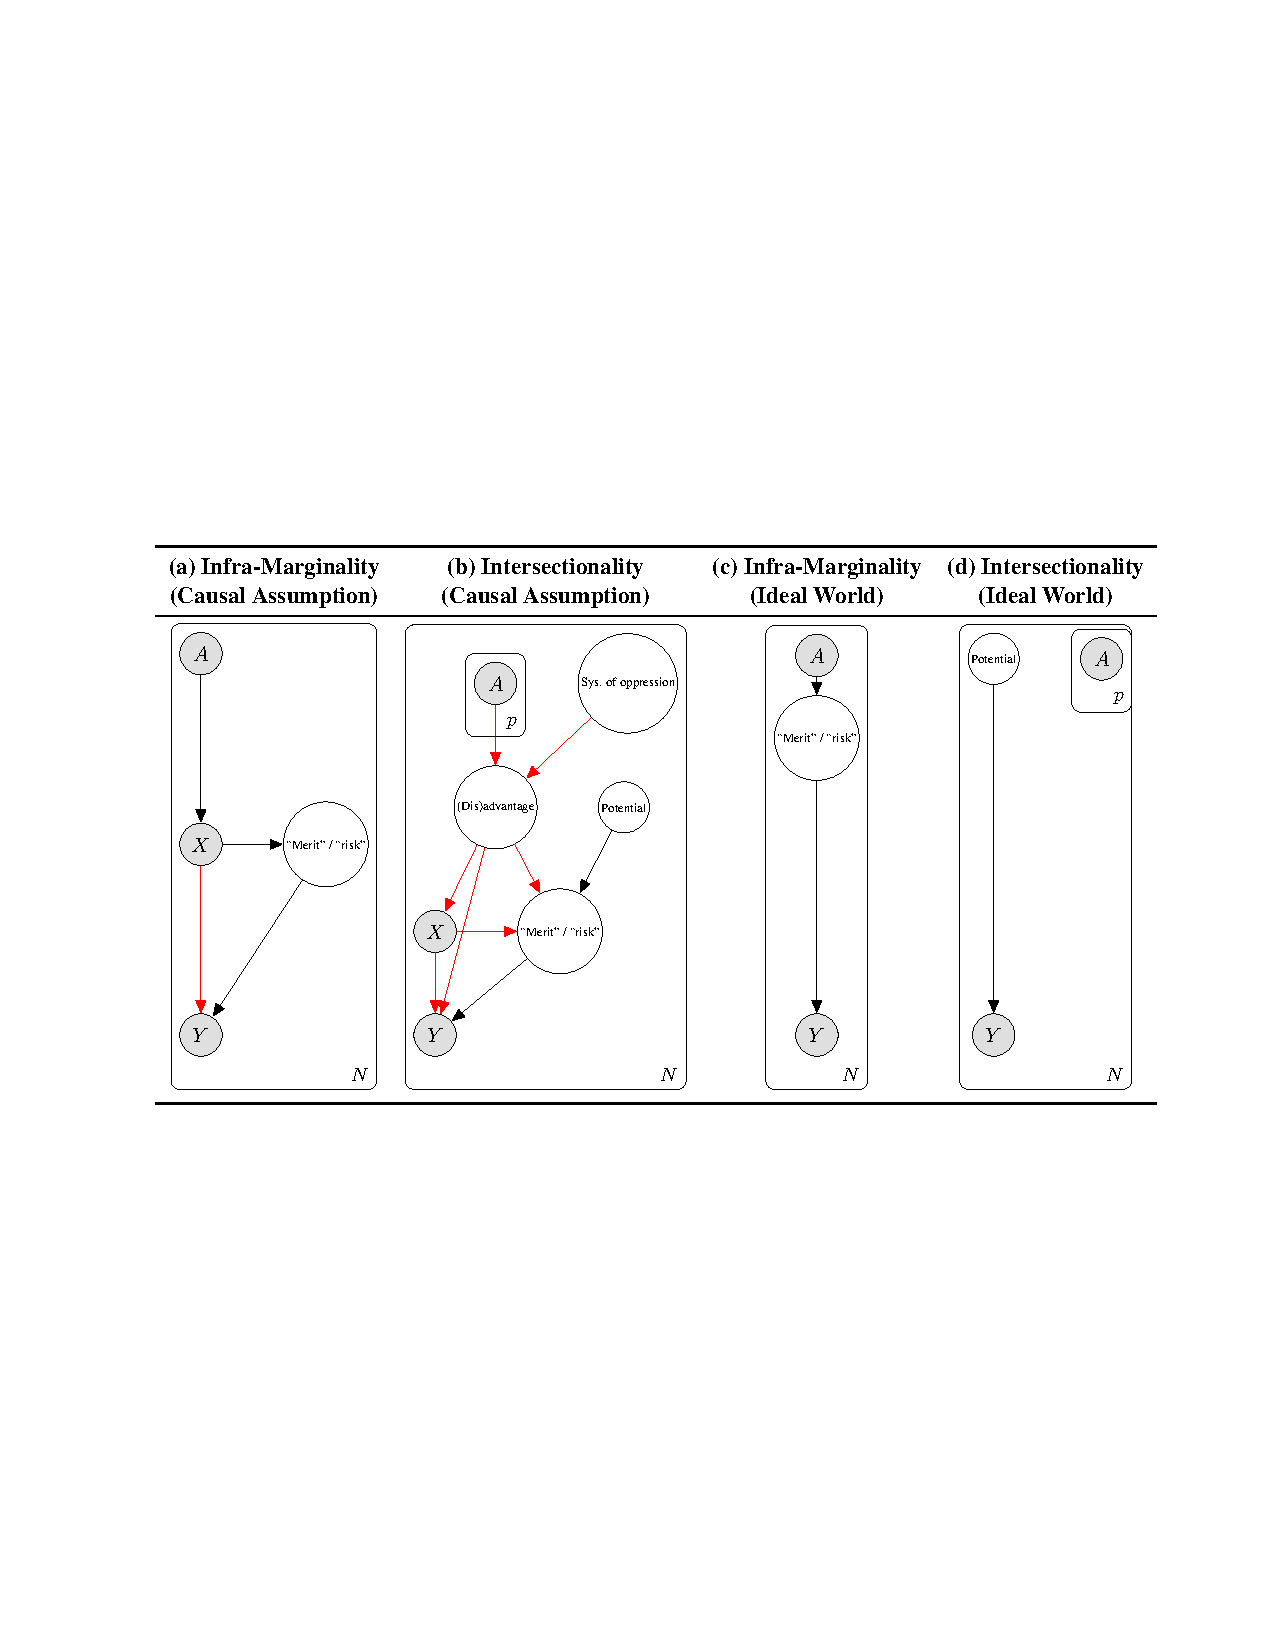
\includegraphics{figs/causalAssumptions.pdf}
	
%The following code generates the figures but isn't compatible with the \documentclass line		
%\begin{tabular}{cccc}
%	\toprule
%	\textbf{(a) Infra-Marginality} & \textbf{(b) Intersectionality} & \textbf{(c) Infra-Marginality} & \textbf{(d) Intersectionality} \\
%	\textbf{(Causal Assumption)} & \textbf{(Causal Assumption)} & \textbf{(Ideal World)} &  \textbf{(Ideal World)} \\ 
%	\midrule
%	\begin{tikzpicture}[y=2.44cm]%[x=2cm,y=3cm]
%		\node[obs] (Y) {$Y$} ;
%		\node[obs, above=of Y] (X) {$X$} ;
%		\node[latent, right=of X] (M) {\tiny ``Merit'' / ``risk''};
%		\node[obs, above=of X] (A) {$A$} ;
%		
%		\edge {A} {X}
%		\edge {X} {M}
%		\edge[red] {X} {Y}
%		\edge {M} {Y}
%		
%		\plate {infraPeople} {(A)(X)(M)(Y)} {$N$}
%	\end{tikzpicture}
%	 &
%	 
%	 \begin{tikzpicture}%[x=2cm,y=1.5cm]	 
%		 \node[obs] (Y) {$Y$} ;
%		 \node[obs, above=of Y] (X) {$X$} ;
%		 \node[latent, right=of X] (M) {\tiny ``Merit'' / ``risk''} ;
%		 \node[latent, above=of X, xshift = 1cm] (P) {\tiny (Dis)advantage} ;
%		 \node[latent, right=of P] (U) {\tiny Potential} ;
%		 \node[obs, above=of P] (A) {$A$} ;
%		 \node[latent, right=of A] (S) {\tiny Sys. of oppression} ;
%		 
%		 
%		 \edge[red] {A,S} {P}
%		 \edge[red] {P} {M}
%		 \edge[] {U} {M}
%		 \edge[red] {P} {X}
%		 \edge[red] {X} {M}
%		 \edge[red] {X} {Y}
%		 \edge {M} {Y}
%		 \edge[red] {P} {Y}
%		 
%		 \plate {interPeople} {(A)(X)(M)(Y)(P)(U)(S)} {$N$}
%		 \plate {interAtts} {(A)} {$p$}
%	 \end{tikzpicture}
%	&
%	\begin{tikzpicture}[y=3.85cm]%[x=2cm,y=3cm]
%		\node[obs] (Y) {$Y$} ;
%		\node[latent, above=of Y] (M) {\tiny ``Merit'' / ``risk''};
%		\node[obs, above=of X] (A) {$A$} ;
%		
%		\edge {A} {M}
%		\edge {M} {Y}
%		
%		\plate {infraIdealPeople} {(A)(M)(Y)} {$N$}	
%	\end{tikzpicture}
%	& 
%	\begin{tikzpicture}[y=5.44cm]%[x=2cm,y=2cm]	 
%	\node[obs] (Y) {$Y$} ;
%	\node[latent, above=of Y] (U) {\tiny Potential} ;
%	\node[obs, right=of U] (A) {$A$} ;	
%	
%	\edge {U} {Y}
%	
%	\plate {interPeople} {(A)(Y)(U)} {$N$}
%	\plate {interAtts} {(A)} {$p$}
%	\end{tikzpicture} \\
%	\bottomrule
%\end{tabular}
}
\caption{Implicit causal assumptions (a,b) and values-driven ideal world scenarios (c,d) for infra-marginality based \cite{corbettdavies2018measure,simoiu2017problem} and intersectionality-based \cite{crenshaw1989demarginalizing, collins2002black} perspectives on fairness \cite{foulds2020intersectional}. Here, $A$ denotes protected attributes, $X$ observed attributes, $Y$ outcomes, $N$ individuals, $p$ number of protected attributes.  Red arrows denote potentially unfair causal pathways, which are removed to obtain the ideal world scenarios (c,d). The above summarizes broad strands of research; individual works may differ. Note that in the intersectionality ideal world, protected attributes are $d$-separated from outcomes, which would imply that parity should occur, while this is not the case in the infra-marginality based ideal world which is willing to accept disparity. \label{fig:causalAssump}}
\end{figure*}


Also note that the inframarginality criticism is only relevant in scenarios where risk scores (or merit / qualifications) are used to assign favorable or unfavorable outcomes.  It does not pertain to other scenarios like recommendation, e.g. AI-based career counseling, where the class labels are not intrinsically better or worse than each other but we would still like to achieve parity \cite{Zeng,islam2020neural}. Lastly, race is a social construct and is not a well-defined biological property \cite{wagner2017anthropologists}.  Similarly, gender (as opposed to biological sex) is also a social construct \cite{west1987doing}.  Although racial and gender groups have diverse sets of lived experiences, there is little scientific evidence that there are legitimate biological differences in the ability levels of these groups \cite{wagner2017anthropologists, ellemers2018gender}.  Insinuations of such differences without clear supporting evidence can potentially veer into the realms of prejudice or scientific racism.

Regarding disparities due to confounders, as in the UC Berkeley graduate admissions case \cite{bickel1975sex}, this is a legitimate concern.  If known confounders exist, fairness methods which account for them should be used instead of simple parity-based methods, e.g. \cite{kusner2017counterfactual,nabi2018fair,nabi2019learning}.  Without complex causal modeling, a simple parity-based approach is to calculate parity-based fairness metrics conditioned on the confounder, as in the \emph{differential fairness with confounders} ($\epsilon$-DFC) metric proposed by the authors \cite{foulds2020intersectional}.  If confounders are unknown, it is difficult to prevent their impact on fairness measures, even ones based on causality, which typically require a causal model to be defined by the analyst.  In this case, we will argue below that the burden of proof for latent confounders may not lie with the organization which is developing the AI system in question.   
%\shimei{Please clarify "organization"} \jf{done} 
Yet, if researchers can identify confounders that impact parity post-deployment, they would be right to ask for the parity-based intervention to be modified or overturned.  Note also that \emph{systemic bias is itself a confounding variable} (cf. Figure \ref{fig:causalAssump} (b)).  If a causal model does not account for it in assessing fair outcomes, its inferences will not be fair or correct, either.  

\subsubsection{Response: Parity does not Prevent Certain Harms or Abuses, or Provide Certain Benefits} 
\label{sec:responseAbuses}

Recall that subset targeting, or fairness gerrymandering, is the issue that parity-based fairness methods do not protect against deliberate (or accidental) bias toward subgroups of the protected groups \cite{dwork2012fairness, kearns2018preventing}.  For example, if we enforce parity for gender and race, groups at the intersection of gender and race such as Black women are not necessarily protected, which is concerning from the perspective of intersectionality \cite{crenshaw1989demarginalizing}.  This problem can be mitigated by simply defining more fine-grained protected groups, e.g. designating Black women as protected.  Sophisticated parity-based fairness metrics have been proposed which automatically enforce parity for groups at the intersection of the protected attributes, including \emph{differential fairness (DF)} \cite{foulds2020intersectional} and \emph{statistical parity (SP) subgroup fairness} \cite{kearns2018preventing}.

Critics of the relationship between parity-based fairness and politically left-wing approaches such as affirmative action, particularly those who are concerned that they will be left behind by these ideas, are recommended to read the book ``\emph{Feminism is for Everybody}'' \cite{hooks2000feminism}.  The authors studied the related concern that \emph{some disadvantaged groups might be harmed by the fairness intervention} \cite{foulds2020intersectional}.  When enforcing our parity-based \emph{differential fairness} metric, which protects intersecting subgroups of protected groups, we found empirically that per-group fairness metrics were improved for almost every subgroup under consideration. 

Some of the other concerns we considered were that parity-based fairness could be achieved by badly behaved classifiers, such as those that deliberately select unqualified individuals to achieve parity, or by increasing negative outcomes.  One response to these types of concerns can be summarized by an old joke:
\begin{quote}
\emph{
``The patient says, `Doctor, it hurts when I do this.' \\
The doctor says, `Then don't do that!' ''} -- Henny Youngman, comedian.\footnote{\url{https://www.goodreads.com/author/quotes/82949.Henny_Youngman}}
\end{quote}
In other words, if these models are considered harmful, we can choose not to create them.    It is not reasonable to expect a single fairness definition to detect and prevent all possible bad behavior.  On the other hand, a healthy process for constructing fair AI should involve an engaged data scientist, plus ideally representatives of stakeholders, who should verify whether the behavior of the model is acceptable or pathological, beyond simply looking at chosen fairness metrics.  Once detected by an analyst, additional problems can be prevented by adding further penalties and constraints to the AI model, in addition to enforcing the parity-based metric.  Note that the \emph{self-fulfilling prophecy} issue (using the consequences of deliberate non-meritocratic parity to justify prejudice) was raised by privacy and security researchers \cite{dwork2012fairness}, whose field has a natural skepticism on human behavior.  While the skepticism may sometimes hold true, we anticipate that the vast majority fairness interventions will be made in good faith. 

Regarding benefits that parity-based fairness metrics do not achieve, such as individual guarantees, these are good reasons to consider using an alternative fairness metric.  They are not, however, reasons to dismiss parity-based fairness metrics out-of-hand as a useful tool for combating bias and fairness issues. For individual guarantees specifically, we would like to point out that parity-based fairness does confer a useful \emph{probabilistic} benefit to the individual: given their protected group, the prior probability of receiving a favorable outcome (before observing any attributes) will be similar to that of an individual from another group.  In the parity-based differential fairness metric \cite{foulds2020intersectional}, this translates to a privacy guarantee \emph{for individuals}: if an adversary sees your outcome $M(x)$, they will not be able to learn much about your protected attribute $s$.  

\subsection{Who has the Burden of Proof on Determining Whether Disparities are Legitimate?}

As we have discussed in Section \ref{sec:responseMeritocracy}, whether parity-based fairness interventions improve or degrade  the extent to which the classifier is meritocratic hinges on whether disparities in the data, which are replicated by the algorithm, are primarily due to unfair bias (from systemic bias, biased data annotation, etc), or are due to legitimate reasons (infra-marginality, confounders, etc).  Since bias is a complicated issue, it is rarely easy to answer this question.  When an organization decides whether or not to implement a parity-based fairness intervention, do they have the burden of proof on showing whether disparities are unfair?  In the absence of solid evidence, which assumption should be the default?

From a legal perspective, in the context of employment decisions in the United States protected by Title VII, if a plaintiff can demonstrate disparate impact (i.e. disparities in outcomes determined by a policy or algorithm), the burden of proof falls on the organization to demonstrate that the disparate impact is justified.  In other words, the organization must justify disparity due to its actions, but it need not justify parity due to its actions.  Thus, from a legal perspective, if the cause of the disparity is unknown it may be safest to assume that the disparity is unfair and apply a parity-based fairness intervention.\footnote{The authors of this paper are not legal experts and the statements in this paper should not be construed as legal advice.}

We may arrive at a similar conclusion from an ethical perspective.  If we incorrectly assume that a disparity is unjust and wrongly remove it, the harm falls on advantaged groups, and diversity/equity (a property which generally has intrinsic value) would be improved.  If we incorrectly assume that a disparity is just and wrongly choose not to address it, the harm falls on disadvantaged groups, and diversity/equity would not be improved.  The advantaged groups  typically have more resources than the disadvantaged groups and are in a better position to shoulder the burden, so the overall impact is less if those groups are harmed.  If we make a wrong choice, meritocracy is harmed either way to the same degree (the size of the intervention).  Therefore, supposing there is a 50/50 or greater chance that the disparity is unjust, the least amount of expected harm occurs if we choose to perform a parity-based fairness intervention.  All other things being equal, in a situation where we have good reason to suspect that a disparity of outcomes is unjust ---such as scientific studies showing discrimination in similar settings--- and we have no reason to suspect that the disparity of outcomes is legitimate ---e.g. one demographic is legitimately more qualified than another or there are known confounders---, performing a parity-based fairness intervention may be a better choice than doing nothing at all, supposing that we do so in a manner that does not substantially harm system performance.  Of course, if there is another fairness intervention that is more appropriate in our particular context, we should consider performing that intervention instead.

\subsection{Summary of our Findings}

Based on the analysis in this paper, we have yet to see a compelling argument that parity-based fairness metrics are invalid in all contexts.  We do not agree with \cite{Hardt2016approaching} that parity-based fairness metrics are ``fundamentally flawed.'' Parity-based fairness advances the intrinsically valuable ideal of equality, can rectify societal bias, can prevent bias from unfair class labels, and has economic and legal benefits in some contexts.  We have also seen that parity-based fairness is not always ideal, and there are a number of useful arguments regarding the limitations of parity-based fairness in some contexts and under some value systems.  The existence of limitations does not however completely preclude its use.  Some of these limitations can be partially mitigated within a parity-based approach, while in other cases may be best addressed by the use of alternative fairness metrics such as equalized odds, individual fairness, or causal fairness definitions.  These alternative fairness metrics have their own limitations, and none can conclusively be argued to be superior to parity-based fairness in all contexts.

% -Must a fairness definition prevent all possible evils to be considered valid, including ones that can be prevented by design or otherwise checked?
%   -Is the goal to achieve (perfect) fairness, or to reduce bias/discrimination?  If we are doing fairness, maybe our metric has to capture what it philosophically means to be fair.  But this seems impossible, especially since fairness is highly contested for centuries, and is highly context dependent.  If we are doing bias reduction, it doesn't matter if our metric is a perfect barometer for justice, as long as it leads to a beneficial intervention. 

% -It isn't fair to dismiss a fairness intervention due to its behavior in the most extreme settings, when more moderate settings can be chosen.

% -In some cases, other metrics are preferable.  That does not mean that parity-based fairness is not a useful construct.

% -``A fairness definition has limitations and does not apply in all contexts'' is not a reason to dismiss it out of hand.  Every fairness definition has limitations, including the competing definitions to parity-based metrics.  If you can imagine a scenario where it is inappropriate, don't use it in that scenario. 

% -For detractors to argue that a fairness metric is too flawed to be used, they must show that it causes more harm than good (or less benefit than alternatives) in all contexts.  They have not done so. 

%Case study: university admissions?

\section{Guidelines and Recommendations}

Informed by the above discussion we now provide a set of guidelines and recommendations to the community regarding parity-based fairness metrics.

\subsection{Guidelines on Using Parity-Based Fairness Interventions}

The technique of penalizing or constraining a machine learning algorithm to enforce a parity-based fairness metric is useful in many contexts, but it must be used with care.  Due to its various limitations, it is not appropriate in all contexts.  We must carefully consider the relevant properties of the AI task at hand and its broader socio-technical context before determining whether to proceed.  We propose the following set of guidelines to be used as a ``pre-flight checklist'' on whether and how to use a parity-based fairness intervention.  This list is only a guideline, not a prescription, and it is almost certainly not complete. It is important to further consider the nuances of the particular application.  Several of these guidelines apply more broadly to all of fair AI. 
 
\begin{enumerate}

 \item When developing an AI fairness intervention, including the choice of fairness metric to uphold in a fair learning algorithm, it is important to consider contextual factors such as who is harmed, what is the nature of the harm, how does it relate to historical injustices, and stakeholder involvement in the design of the fair AI system, particularly stakeholders who are underrepresented within the organization \cite{crawford2019ai}.
 
 \item Before using any fairness intervention or deploying a fairness-sensitive system without one, practitioners should make a best-effort attempt to understand whether disparities of class labels in the data are substantially due to unfair reasons or to legitimate reasons.  If this cannot be determined from available data, scientific studies on related settings may suggest whether unfair bias is likely in the current context.
 
 \item If the disparity is due to legitimate reasons, e.g. there are known legitimate differences in ability between groups (infra-marginality), parity-based fairness metrics are not appropriate.  Consider using threshold tests instead. 

 \item If there are known confounders, parity-based fairness metrics are not appropriate.  Parity-based metrics which account for confounders such as $\epsilon$-DFC, or causal methods, should be used instead.
 
 \item If strong individual-level guarantees are essential for the application, individual fairness should be used instead.  Similarly, if there are other essential fairness properties that are only ensured by a different definition, that definition should be used instead. 

 \item If harm by the system is due to making prediction errors rather than from not receiving a favorable outcome, equalized odds or equality of opportunity are more appropriate fairness definitions.
 
 \item If it is suspected that disparities of class labels are substantially unfair (e.g. due to societal bias or annotation bias), disparities cause a harm of representation, or equality is important for the application regardless of unfairness in the data, parity-based fairness metrics are a good candidate to be used.
 
 \item If there is uncertainty over whether disparities of class labels are unfair, but there is reasonable suspicion that this is the case and there is no evidence of infra-marginality or confounding, it may be better to perform a parity-based fairness intervention than to make no fairness intervention.  Wrongly making a parity-based fairness intervention may be less harmful than wrongly failing to make a parity-based fairness intervention.  This assumes that the intervention is done such that little reduction in accuracy occurs, and that there is not another more appropriate fairness intervention for this context. 
 
 \item If it is important to maintain a high level of classification accuracy for this application, choose appropriate fairness hyper-parameter settings to achieve this.  We generally recommend using a grid search on a validation set to select fairness hyper-parameters, such that fairness is the best achievable under the constraint that accuracy decrease (or another performance metric) is within (say) 95\% of the performance of the typical model (accuracy $\times \ 0.95$).
 
 \item If no loss in accuracy at all is acceptable, consider setting a threshold on the fairness penalty such that only an increase in disparity over the existing disparity in the data is penalized.  This strategy only prevents ``bias amplification'' due to the algorithm's behavior, e.g. from overfitting.
 
 \item If we have strong evidence that most of the disparity is due to unfair reasons, a strict parity-based fairness constraint may be appropriate, even at a substantial cost to accuracy, since an accurate classifier cannot be a fair one in that case.
  
 \item After deployment, it is important to continue to monitor the fairness of the system and to continue to learn about the nature of the unfairness in the data and the system, and adapt the intervention accordingly.  For example, if external researchers or activists identify a flaw in the fairness of the system, corresponding adjustments should be made. 


\end{enumerate}
  
\subsection{Recommendations to the Community}

After considering the many arguments on both sides of the issue, we conclude that parity-based fairness metrics remain a valid and desirable notion of fair AI behavior in many 
%\shimei{How about replacing "some" with "many"?}\jf{done}
contexts.  We therefore \textbf{call upon community members 
%\shimei{how about replacing "peer reviewers" with "community members" since  not just "peer reviewers" need to pay attention to this }\jf{done.  I instead mentioned peer review as important in the next sentence, though. I emphasize it because I want this paper to be a reference for authors to use in their rebuttals if they encounter these criticisms during peer review}
to cease the practice of dismissing fundamental methods-oriented AI fairness research on parity-based fairness metrics out-of-hand}, due to perceived limitations of the approach. \emph{This is particularly important during peer review}.  It is however appropriate to critique \emph{applied AI fairness research} 
%\shimei{How about removing "during peer review". Although it is important in terms of publication, most people care more about the real impact of deployed systems than publications. }\jf{done}
regarding the limitations of any chosen fairness metric (parity-based or otherwise) relative to alternatives \emph{in the context of a particular application}, as long as political impartiality is maintained as much as possible.  For example, debate and critiques regarding the appropriate metrics to evaluate the fairness of the COMPAS criminal recidivism predictor \cite{angwin2016machine} are valuable and would have been appropriate in peer review of a paper describing the COMPAS system.  We request that peer reviewers endeavor to prevent their own political views and value systems from impacting their assessment of AI fairness research.

We further suggest that the debate around parity-based fairness  should remain civil in highly public settings such as in audience questions after conference talks and on social media.  In those contexts there are often impassioned, sometimes even angrily stated objections to parity-based fairness, as the authors of this paper have witnessed first-hand.  The presently ongoing debate around the firing of Timnit Gebru by Google is emblematic of the high tensions in this area.  While debate around these issues must continue and we do not intend to stifle it, unjustified vitriolic attacks on parity-based fairness research can have a chilling effect on a much-needed area of study, and they do nothing to advance the discussion. 
%\shimei{Again, conference Q\&A sessions or even social media can be an appropriate venue for this type of discussion/debate/criticism as long as people remain civil. Otherwise, where should the debate/discussion occur? Suggest to remove the part in the above paragraph that sounds personal.} \jf{I modified to simply request civility.  I have left in the personal part but I rearranged the sentence to reduce the importance of the personal dimension.  It is there to support the claim - we have seen first hand that this happens, so we don't need to cite other evidence for it.}
%\shimei{Thank you for the revision. I like the current version much better.}
%JF: ok, commenting this out since it seems to be addressed.


% \begin{figure}
% 	\centering
% 	
\includegraphics{figs/myfigure.png}
	
% 	\caption{An example figure.}
	
% \end{figure}
 

\section{Conclusions}
Despite their widespread use, parity-based AI fairness metrics have been somewhat controversial in some circles due to various limitations that have been put forward in the literature.  We discussed the pros and cons of these metrics when used as a penalty or constraint to enforce AI fairness in a machine learning system.  In many contexts, parity-based fairness confers useful benefits such as mitigating unfair disparities, improving diversity, and reducing legal liability.  Although many important concerns have been raised such as potentially reducing prediction accuracy or unfair impacts when they are used to remove legitimate disparities, mitigation strategies exist, and none of the concerns would preclude the use of the methodology in all contexts.  We conclude that although parity-based fairness metrics are not a panacea, and there are situations where they are not appropriate or other fairness metrics would be preferable, they remain useful tools in the AI fairness practitioner's toolkit.

\section{Acknowledgments}
We thank Rosie Kar for valuable insights regarding intersectionality and standpoint theory. This work was performed under the following financial assistance award: 60NANB18D227 from U.S. Department of Commerce, National Institute of Standards and Technology. This material is based upon work supported by the National Science Foundation under Grant Nos IIS 1850023; IIS1927486.  Any opinions, findings, and conclusions or recommendations expressed in this material are those of the author(s) and do not necessarily reflect the views of the National Science Foundation.

\newpage
 
\vspace{-.1cm}
%\bibliographystyle{ACM-Reference-Format}
%\bibliographystyle{apalike}
%\bibliography{references}

\begin{thebibliography}{}
	
	\bibitem[Alexander, 2012]{alexander2012new}
	Alexander, M. (2012).
	\newblock {\em The new Jim Crow: Mass incarceration in the age of
		colorblindness}.
	\newblock T. N. P.
	
	\bibitem[Angwin et~al., 2016]{angwin2016machine}
	Angwin, J., Larson, J., Mattu, S., and Kirchner, L. (2016).
	\newblock Machine bias: There's software used across the country to predict
	future criminals. and it's biased against blacks.
	\newblock {\em ProPublica, May}, 23.
	
	\bibitem[Ayres, 2002]{ayres2002outcome}
	Ayres, I. (2002).
	\newblock Outcome tests of racial disparities in police practices.
	\newblock {\em Justice research and Policy}, 4(1-2):131--142.
	
	\bibitem[Barocas and Selbst, 2016]{barocas2016big}
	Barocas, S. and Selbst, A. (2016).
	\newblock Big data's disparate impact.
	\newblock {\em Cal. L. Rev.}, 104:671.
	
	\bibitem[Barrett et~al., 2019]{barrett2019emotional}
	Barrett, L.~F., Adolphs, R., Marsella, S., Martinez, A.~M., and Pollak, S.~D.
	(2019).
	\newblock Emotional expressions reconsidered: Challenges to inferring emotion
	from human facial movements.
	\newblock {\em Psychological science in the public interest}, 20(1):1--68.
	
	\bibitem[Beede et~al., 2011]{beede2011women}
	Beede, D.~N., Julian, T.~A., Langdon, D., McKittrick, G., Khan, B., and Doms,
	M.~E. (2011).
	\newblock Women in stem: A gender gap to innovation.
	\newblock {\em Economics and Statistics Administration Issue Brief}, 04-11.
	
	\bibitem[Bell et~al., 2011]{bell2011voice}
	Bell, M.~P., {\"O}zbilgin, M.~F., Beauregard, T.~A., and S{\"u}rgevil, O.
	(2011).
	\newblock Voice, silence, and diversity in 21st century organizations:
	Strategies for inclusion of gay, lesbian, bisexual, and transgender
	employees.
	\newblock {\em Human resource management}, 50(1):131--146.
	
	\bibitem[Berk et~al., 2018]{berk2017fairness}
	Berk, R., Heidari, H., Jabbari, S., Kearns, M., and Roth, A. (2018).
	\newblock Fairness in criminal justice risk assessments: The state of the art.
	\newblock {\em In Sociological Methods and Research}, 1050:28.
	
	\bibitem[Bickel et~al., 1975]{bickel1975sex}
	Bickel, P.~J., Hammel, E.~A., and O'Connell, J.~W. (1975).
	\newblock Sex bias in graduate admissions: Data from {B}erkeley.
	\newblock {\em Science}, 187(4175):398--404.
	
	\bibitem[Buolamwini and Gebru, 2018]{buolamwini2018gender}
	Buolamwini, J. and Gebru, T. (2018).
	\newblock Gender shades: Intersectional accuracy disparities in commercial
	gender classification.
	\newblock In {\em FAT*}.
	
	\bibitem[Collins, 1990]{collins2002black}
	Collins, P. (2002 [1990]).
	\newblock {\em Black feminist thought: Knowledge, consciousness, and the
		politics of empowerment (2nd ed.)}.
	\newblock Routledge.
	
	\bibitem[{Combahee River Collective}, 1978]{collective1977black}
	{Combahee River Collective} (1978).
	\newblock A {B}lack feminist statement.
	\newblock In Eisenstein, Z., editor, {\em Capitalist Patriarchy and the Case
		for Socialist Feminism}. Monthly Review Press, New York.
	
	\bibitem[Corbett-Davies and Goel, 2018]{corbettdavies2018measure}
	Corbett-Davies, S. and Goel, S. (2018).
	\newblock The measure and mismeasure of fairness: A critical review of fair
	machine learning.
	
	\bibitem[Cox and Blake, 1991]{cox1991managing}
	Cox, T.~H. and Blake, S. (1991).
	\newblock Managing cultural diversity: Implications for organizational
	competitiveness.
	\newblock {\em Academy of Management Perspectives}, 5(3):45--56.
	
	\bibitem[Crawford et~al., 2019]{crawford2019ai}
	Crawford, K., Dobbe, R., Dryer, T., Fried, G., Green, B., Kaziunas, E., Kak,
	A., Mathur, V., McElroy, E., S{\'a}nchez, A.~N., et~al. (2019).
	\newblock {AI} {N}ow 2019 report.
	\newblock {\em New York, NY: AI Now Institute}.
	
	\bibitem[Crenshaw, 1989]{crenshaw1989demarginalizing}
	Crenshaw, K. (1989).
	\newblock Demarginalizing the intersection of race and sex: A {B}lack feminist
	critique of antidiscrimination doctrine, feminist theory and antiracist
	politics.
	\newblock {\em U. Chi. Legal F.}, pages 139--167.
	
	\bibitem[Dastin, 2018]{dastin2018amazon}
	Dastin, J. (2018).
	\newblock Amazon scraps secret {AI} recruiting tool that showed bias against
	women.
	\newblock {\em Reuters}.
	
	\bibitem[Davis, 2011]{davis2011prisons}
	Davis, A. (2011).
	\newblock {\em Are prisons obsolete?}
	\newblock Seven Stories Press.
	
	\bibitem[Deshpande et~al., 2020]{ketki}
	Deshpande, K.~V., Pan, S., and Foulds, J.~R. (2020).
	\newblock Mitigating demographic bias in {AI}-based resume filtering.
	\newblock In {\em UMAP '20 Adjunct}, page 268–275. Association for Computing
	Machinery.
	
	\bibitem[Dionne, 2004]{dionne2004americans}
	Dionne, E.~J. (2004).
	\newblock {\em Why Americans hate politics}.
	\newblock Simon and Schuster.
	
	\bibitem[Dwork et~al., 2012]{dwork2012fairness}
	Dwork, C., Hardt, M., Pitassi, T., Reingold, O., and Zemel, R. (2012).
	\newblock Fairness through awareness.
	\newblock In {\em Proceedings of ITCS}, pages 214--226.
	
	\bibitem[Ellemers, 2018]{ellemers2018gender}
	Ellemers, N. (2018).
	\newblock Gender stereotypes.
	\newblock {\em Annual review of psychology}, 69:275--298.
	
	\bibitem[{Equal Employment Opportunity Commission}, 1978]{eeoc1966guidelines}
	{Equal Employment Opportunity Commission} (1978).
	\newblock Guidelines on employee selection procedures.
	\newblock {\em C.F.R.}, 29.1607.
	
	\bibitem[Foulds et~al., 2020]{foulds2020bayesian}
	Foulds, J.~R., Islam, R., Keya, K.~N., and Pan, S. (2020).
	\newblock Bayesian modeling of intersectional fairness: The variance of bias.
	\newblock In {\em Proceedings of the 2020 SIAM International Conference on Data
		Mining}, pages 424--432. SIAM.
	
	\bibitem[{Foulds} et~al., 2020]{foulds2020intersectional}
	{Foulds}, J.~R., {Islam}, R., {Keya}, K.~N., and {Pan}, S. (2020).
	\newblock An intersectional definition of fairness.
	\newblock In {\em 2020 IEEE 36th International Conference on Data Engineering
		(ICDE)}, pages 1918--1921.
	
	\bibitem[Grant et~al., 2011]{grant2011injustice}
	Grant, J., Mottet, L., Tanis, J., Harrison, J., Herman, J., and Keisling, M.
	(2011).
	\newblock {\em Injustice at every turn: A report of the national transgender
		discrimination survey}.
	\newblock National Center for Transgender Equality.
	
	\bibitem[Hardt, 2016]{Hardt2016approaching}
	Hardt, M. (2016).
	\newblock Approaching fairness in machine learning.
	\newblock [Online; posted September 6, 2016]
	\url{http://blog.mrtz.org/2016/09/06/approaching-fairness.html}.
	
	\bibitem[Hardt et~al., 2016]{hardt2016equality}
	Hardt, M., Price, E., Srebro, N., et~al. (2016).
	\newblock Equality of opportunity in supervised learning.
	\newblock In {\em Advances in NeurIPS}, pages 3315--3323.
	
	\bibitem[Hartsock, 1983]{hartsock1983feminist}
	Hartsock, N.~C. (1983).
	\newblock The feminist standpoint: Developing the ground for a specifically
	feminist historical materialism.
	\newblock In {\em Discovering reality}, pages 283--310. Springer.
	
	\bibitem[hooks, 1981]{hooks1981ain}
	hooks, b. (1981).
	\newblock {\em Ain't {I} a Woman: Black Women and Feminism}.
	\newblock South End Press.
	
	\bibitem[hooks, 2000]{hooks2000feminism}
	hooks, b. (2000).
	\newblock {\em Feminism is for everybody: Passionate politics}.
	\newblock Pluto Press.
	
	\bibitem[Islam et~al., 2020]{islam2020neural}
	Islam, R., Keya, K.~N., Zeng, Z., Pan, S., and Foulds, J. (2020).
	\newblock Neural fair collaborative filtering.
	
	\bibitem[Jefferson, 2018]{constitution}
	Jefferson, T. (2018).
	\newblock {\em The Papers of Thomas Jefferson, Volume 21: Index}, volume~1.
	\newblock Princeton University Press.
	
	\bibitem[Johnson, 1965]{johnson1965remarks}
	Johnson, L.~B. (1965).
	\newblock {\em Commencement Address at Howard University: ``To Fulfill These
		Rights''}.
	\newblock Howard University.
	
	\bibitem[Kearns et~al., 2018]{kearns2018preventing}
	Kearns, M., Neel, S., Roth, A., and Wu, Z. (2018).
	\newblock Preventing fairness gerrymandering: Auditing and learning for
	subgroup fairness.
	\newblock In {\em Proc. of ICML, PMLR 80}, pages 2569--2577.
	
	\bibitem[Kearns et~al., 2019]{kearns2019average}
	Kearns, M., Roth, A., and Sharifi-Malvajerdi, S. (2019).
	\newblock Average individual fairness: Algorithms, generalization and
	experiments.
	\newblock In {\em Advances in Neural Information Processing Systems}, pages
	8242--8251.
	
	\bibitem[Keya et~al., 2020]{keya2020equitable}
	Keya, K.~N., Islam, R., Pan, S., Stockwell, I., and Foulds, J.~R. (2020).
	\newblock Equitable allocation of healthcare resources with fair {C}ox models.
	
	\bibitem[Keyes et~al., 2019]{keyes2019mulching}
	Keyes, O., Hutson, J., and Durbin, M. (2019).
	\newblock A mulching proposal: Analysing and improving an algorithmic system
	for turning the elderly into high-nutrient slurry.
	\newblock In {\em Extended Abstracts of the 2019 CHI Conference on Human
		Factors in Computing Systems}. ACM.
	
	\bibitem[Kusner et~al., 2017]{kusner2017counterfactual}
	Kusner, M., Loftus, J., Russell, C., and Silva, R. (2017).
	\newblock Counterfactual fairness.
	\newblock In {\em NeurIPS}.
	
	\bibitem[Landeau, 2020]{Landeau2020}
	Landeau, A. (2020).
	\newblock Measuring fairness in machine learning models.
	\newblock [Online; posted September 18-2020].
	
	\bibitem[Lorde, 1984]{lorde1984age}
	Lorde, A. (1984).
	\newblock Age, race, class, and sex: Women redefining difference.
	\newblock In {\em Sister Outsider}, pages 114--124. Ten Speed Press.
	
	\bibitem[Lowry and Macpherson, 1988]{lowry1988blot}
	Lowry, S. and Macpherson, G. (1988).
	\newblock A blot on the profession.
	\newblock {\em British medical journal (Clinical research ed.)}, 296(6623):657.
	
	\bibitem[Nabi et~al., 2019]{nabi2019learning}
	Nabi, R., Malinsky, D., and Shpitser, I. (2019).
	\newblock Learning optimal fair policies.
	\newblock {\em Proceedings of machine learning research}, 97:4674.
	
	\bibitem[Nabi and Shpitser, 2018]{nabi2018fair}
	Nabi, R. and Shpitser, I. (2018).
	\newblock Fair inference on outcomes.
	\newblock In {\em Proceedings of the AAAI Conference on Artificial
		Intelligence}, volume 2018, page 1931.
	
	\bibitem[Nedlund, 2019]{applecard}
	Nedlund, E. (2019).
	\newblock Apple card is accused of gender bias. here's how that can happen.
	\newblock [CNN Business. Online; posted November 12,2019]
	\url{https://www.cnn.com/2019/11/12/business/apple-card-gender-bias/index.html}.
	
	\bibitem[Noble, 2018]{noble2018algorithms}
	Noble, S. (2018).
	\newblock {\em Algorithms of Oppression: How Search Engines Reinforce Racism}.
	\newblock NYU Press.
	
	\bibitem[Page, 2008]{page2008difference}
	Page, S.~E. (2008).
	\newblock {\em The difference: How the power of diversity creates better
		groups, firms, schools, and societies-new edition}.
	\newblock Princeton University Press.
	
	\bibitem[Simoiu et~al., 2017]{simoiu2017problem}
	Simoiu, C., Corbett-Davies, S., Goel, S., et~al. (2017).
	\newblock The problem of infra-marginality in outcome tests for discrimination.
	\newblock {\em The Annals of Applied Statistics}, 11(3):1193--1216.
	
	\bibitem[Truth, 1851]{truth1851aint}
	Truth, S. (1851).
	\newblock Ain't {I} a woman?
	\newblock Speech delivered at Women's Rights Convention, Akron, Ohio.
	
	\bibitem[Vanian, 2019]{HateSpeechDetectionBias}
	Vanian, J. (2019).
	\newblock Google’s hate speech detection {A.I.} has a racial bias problem.
	\newblock [Fortune. Online; posted August 16, 2019]
	\url{https://fortune.com/2019/08/16/google-jigsaw-perspective-racial-bias/}.
	
	\bibitem[Verma and Rubin, 2018]{20plusdefinitionssuervey}
	Verma, S. and Rubin, J. (2018).
	\newblock Fairness definitions explained.
	\newblock In {\em Proceedings of the International Workshop on Software
		Fairness}, pages 1--7. Association for Computing Machinery.
	
	\bibitem[Verschelden, 2017]{verschelden2017bandwidth}
	Verschelden, C. (2017).
	\newblock {\em Bandwidth Recovery: Helping Students Reclaim Cognitive Resources
		Lost to Poverty, Racism, and Social Marginalization}.
	\newblock Stylus.
	
	\bibitem[Wagner et~al., 2017]{wagner2017anthropologists}
	Wagner, J.~K., Yu, J.-H., Ifekwunigwe, J.~O., Harrell, T.~M., Bamshad, M.~J.,
	and Royal, C.~D. (2017).
	\newblock Anthropologists' views on race, ancestry, and genetics.
	\newblock {\em American Journal of Physical Anthropology}, 162(2):318--327.
	
	\bibitem[Weisskopf, 2004]{weisskopf2004affirmative}
	Weisskopf, T.~E. (2004).
	\newblock {\em Affirmative action in the United States and India: A comparative
		perspective}.
	\newblock Routledge.
	
	\bibitem[West and Zimmerman, 1987]{west1987doing}
	West, C. and Zimmerman, D.~H. (1987).
	\newblock Doing gender.
	\newblock {\em Gender \& society}, 1(2):125--151.
	
	\bibitem[Zafar et~al., 2017a]{zafar2015fairness}
	Zafar, M., Valera, I., Rodriguez, M., and Gummadi, K. (2017a).
	\newblock Fairness constraints: Mechanisms for fair classification.
	\newblock In {\em AISTATS}.
	
	\bibitem[Zafar et~al., 2017b]{zafar2017parity}
	Zafar, M.~B., Valera, I., Rodriguez, M., Gummadi, K., and Weller, A. (2017b).
	\newblock From parity to preference-based notions of fairness in
	classification.
	\newblock In {\em Advances in Neural Information Processing Systems}, pages
	229--239.
	
	\bibitem[Zeng et~al., 2021]{Zeng}
	Zeng, Z., Islam, R., Keya, K., Foulds, J., Song, Y., and Pan., S. (2021).
	\newblock Fair heterogeneous network embeddings.
	\newblock In {\em Proceedings of the 15th International AAAI Conference on Web
		and Social Media (Accepted)}. AAAI.
	
	\bibitem[Zhao et~al., 2017]{zhao2017men}
	Zhao, J., Wang, T., Yatskar, M., Ordonez, V., and Chang, K.-W. (2017).
	\newblock Men also like shopping: Reducing gender bias amplification using
	corpus-level constraints.
	\newblock In {\em Proceedings of EMNLP}.
	
\end{thebibliography}



%%%%% Example bibliography using bibitems
% \begin{thebibliography}{10}
% \begin{small}
% \itemsep=-.5pt
% \bibitem{1}
% Athanassoulis, Manos ; Johnson, Ryan ; Ailamaki, Anastasia ; Stoica, Radu, Improving OLTP Concurrency through Early Lock Release, EPFL-REPORT-152158, https://infoscience.epfl.ch/record/152158?ln=en, 2009. 

% \bibitem{2}
% Azure CosmosDB, https://azure.microsoft.com/en-us/services/cosmos-db/ 

% \bibitem{3}
% Bernstein, P.A., M., T. Kiefer, D. Maier: Indexing in an Actor-Oriented Database. CIDR 2017  

% \bibitem{4}
% Bernstein, P. A., E. Newcomer: Chapter 10: Transactional Middleware Products and Standards, in Principles of Transaction Processing, Morgan Kaufmann, 2nd ed., 2009. 

% \bibitem{5}
% Chang, F., J. Dean, S. Ghemawat, W.C. Hsieh, D.A. Wallach, M. Burrows, T. Chandra, A. Fikes, R.E. Gruber: Bigtable: A Distributed Storage System for Structured Data. ACM Trans. Comput. Syst. 26(2): 4:1-4:26 (2008) 


% \bibitem{6}
% %Corbett, J.C., J. Dean, M. Epstein, A. Fikes, C. Frost, J.J. Furman, S. Ghemawat, A. Gubarev, C. Heiser, P. Hochschild, W.C. Hsieh, S. Kanthak, E. Kogan, H. Li, A. Lloyd, S. Melnik, D. Mwaura, D. Nagle, S. Quinlan, R. Rao, L. Rolig, Y. Saito, M. Szymaniak, C. Taylor, R. Wang, D. Woodford: Spanner: Google's Globally Distributed Database. ACM Trans. Comput. Syst. 31(3): 8:1-8:22 (2013) 
% Corbett, J.C. et al: Spanner: Google's Globally Distributed Database. ACM Trans. Comput. Syst. 31(3): 8:1-8:22 (2013) 
% \bibitem{7}
% DeWitt, D.J., R.H. Katz, F. Olken, L.D. Shapiro, M. Stonebraker, D.A. Wood: Implementation Techniques for Main Memory Database Systems. SIGMOD 1984: 1-8 

% \bibitem{8}
% DynamoDB, https://aws.amazon.com/dynamodb/ 

% \bibitem{9}
% Eldeeb, T. and P. Bernstein: Transactions for Distributed Actors in the Cloud. Microsoft Research Tech Report MSR-TR-2016-1001. 

% \bibitem{10}
% Graefe, G., M. Lillibridge, H. A. Kuno, J. Tucek, A.C. Veitch: Controlled lock violation. SIGMOD 2013: 85-96 

% \bibitem{11}
% Helland, P., Life beyond Distributed Transactions: an Apostate's Opinion. CIDR 2007: 132-141 

% \bibitem{12}
% Java EE documentation, http://www.oracle.com/technetwork/?java/javaee/documentation/index.html  

% \bibitem{13}
% Larson, P-A, et al.: High-Perf. Concurrency Control Mechanisms for Main-Memory Databases. PVLDB 2011 
% \bibitem{14}

% Levandoski, L.J., D.B. Lomet, S. Sengupta, R. Stutsman, R. Wang: High Performance Transactions in Deuteronomy. CIDR 2015 

% \bibitem{15}
% David B. Lomet: Using Timestamping to Optimize Two Phase Commit. PDIS 1993: 48-55 

% \bibitem{16}
% Orleans, http://dotnet.github.io/orleans 

% \bibitem{18}
% The Open Group, Distributed Transaction Processing: The XA Specification, http://pubs.opengroup.org/onlinepubs/009680699/toc.pdf. 

% \bibitem{19}
% Vogels W., Eventually Consistent. ACM Queue 6(6): 14-19 (2008) \end{small}
% \end{thebibliography}

\end{document}

\end{article}

%\makeatletter
%\renewcommand{\AB@affillist}{}
%\renewcommand{\AB@authlist}{}
%\setcounter{authors}{0}
%\makeatother
%
\begin{article}
{Trimming the Thorns of AI Fairness Research}
{Jared Sylvester and Edward Raff}
\graphicspath{{submissions/sylvester_raff_final/}}
\documentclass[11pt]{article}
%\documentclass[11pt]{article} %The above line must be used for your camera-ready submission, which requires a latex -> DVI -> PDF compilation pipeline.  As a workaround while you are writing your paper, you could comment it out and use this line instead, which is compatible with pdflatex.
\usepackage{deauthor,times,graphicx} 
%\usepackage[numbers]{natbib}
% \documentclass{article}
% Recommended, but optional, packages for figures and better typesetting:
\usepackage{microtype}
\usepackage{graphicx}
% \usepackage{subfigure}
\usepackage{booktabs} % for professional tables
%\usepackage[table,dvipsnames]{xcolor}
\usepackage{epsfig}
\usepackage{pgfplotstable}
\usepackage{pgfplots}
\usepgfplotslibrary{groupplots}
\usepackage{amsmath}
\usepackage{amssymb}
\usepackage{bbm}
% \usepackage{minted}
\usepackage{float}
% \usepackage{tikz}
% \usetikzlibrary{decorations.text,calc,shapes,arrows,arrows.meta, positioning,shapes.misc,decorations.markings,decorations.markings,decorations.pathreplacing,matrix}
\usepackage{booktabs}
% \usepackage{multirow}
% \usepackage{adjustbox}
\usepackage{verbatim}
%\usepackage[T1]{fontenc}
% \usepackage[title]{appendix}
\usepackage{graphicx}
\usepackage{caption}
% \usepackage{algpseudocode}
% \usepackage{algorithm}
% \usepackage{paralist} %Compact lists 
\usepackage{siunitx}
% \usepackage{nicefrac}
\usepackage{xspace}
%\usepackage[colorinlistoftodos,textsize=footnotesize]{todonotes}

%\usepackage[utf8]{inputenc}

\newcommand{\textcite}[1]{\citet{#1}}


%let me use normal quotation marks
%\usepackage[autostyle, english=american]{csquotes}
\MakeOuterQuote{"}

%fix long URLs in bib
\usepackage{url}
\def\UrlBreaks{\do\/\do-}
\usepackage{breakurl}

% hyperref makes hyperlinks in the resulting PDF.
% If your build breaks (sometimes temporarily if a hyperlink spans a page)
% please comment out the following usepackage line and replace
% \usepackage{icml2018} with \usepackage[nohyperref]{icml2018} above.
% \usepackage[draft]{hyperref}
%\usepackage[hidelinks,pdftitle={Trimming the Thorns of AI Fairness Research},pdfauthor={Sylvester \& Raff}]{hyperref}

% Attempt to make hyperref and algorithmic work together better:
\newcommand{\theHalgorithm}{\arabic{algorithm}}

% Use the following line for the initial blind version submitted for review:
% \usepackage{icml2018}
% \usepackage[nohyperref]{icml2018}

% If accepted, instead use the following line for the camera-ready submission:
% \usepackage[accepted]{icml2018}

% The \icmltitle you define below is probably too long as a header.
% Therefore, a short form for the running title is supplied here:
% \icmltitlerunning{Applied Fairness, Page \thepage} % comment this out to get page numbers in header instead


% \everypar{\looseness=-1 } %Please try and avoid dangling words on their own lines! 
% \linepenalty=2000 %Please avoid white space! 
\clubpenalty=10000
\widowpenalty=10000

% \setlength{\textfloatsep}{12pt plus 4pt minus 6pt}

% \renewcommand\floatpagefraction{.9}
% \renewcommand\dblfloatpagefraction{.9} % for two column documents
% \renewcommand\topfraction{.9}
% \renewcommand\dbltopfraction{.9} % for two column documents
% \renewcommand\bottomfraction{.9}
% \renewcommand\textfraction{.1}   

\begin{document} 
% Trimming the Thorns of AI Fairness Research
% Making AI Fairness Research Constructive and Accessible
\title{Trimming the Thorns of AI Fairness Research}
\author{
  Jared Sylvester\\
  Independent\\
  \texttt{j@jsylvest.com}
  \and
  Edward Raff\\
  Booz Allen Hamilton\\
  \texttt{Raff\_Edward@bah.com}
}

% \twocolumn[
% \icmltitle{What About Applied Fairness? }

% It is OKAY to include author information, even for blind
% submissions: the style file will automatically remove it for you
% unless you've provided the [accepted] option to the icml2018
% package.

% List of affiliations: The first argument should be a (short)
% identifier you will use later to specify author affiliations
% Academic affiliations should list Department, University, City, Region, Country
% Industry affiliations should list Company, City, Region, Country

% You can specify symbols, otherwise they are numbered in order.
% Ideally, you should not use this facility. Affiliations will be numbered
% in order of appearance and this is the preferred way.
% \icmlsetsymbol{equal}{*}

% \begin{icmlauthorlist}
%   \icmlauthor{Jared Sylvester}{bah}
%   \icmlauthor{Edward Raff}{bah,umbc}
% \end{icmlauthorlist}

% \icmlaffiliation{bah}{Booz Allen Hamilton}
% \icmlaffiliation{umbc}{University of Maryland, Baltimore County}

% \icmlcorrespondingauthor{Edward Raff}{raff\_edward@bah.com}

% % You may provide any keywords that you
% % find helpful for describing your paper; these are used to populate
% % the "keywords" metadata in the PDF but will not be shown in the document
% \icmlkeywords{Machine Learning, ICML}

% \vskip 0.3in
% ]

% this must go after the closing bracket ] following \twocolumn[ ...

% This command actually creates the footnote in the first column
% listing the affiliations and the copyright notice.
% The command takes one argument, which is text to display at the start of the footnote.
% The \icmlEqualContribution command is standard text for equal contribution.
% Remove it (just {}) if you do not need this facility.

% \printAffiliationsAndNotice{}  % leave blank if no need to mention equal contribution
% \printAffiliationsAndNotice{\icmlEqualContribution} % otherwise use the standard text.
\maketitle
\begin{abstract}

Machine learning practitioners are often ambivalent about the ethical aspects of their products. We believe anything that gets us from that current state to one in which our systems are achieving some degree of fairness is an improvement that should be welcomed. This is true even when that progress does not get us 100\% of the way to the goal of "complete" fairness or perfect alignment with our personal belief on which measure of fairness is used. Systems being built with some measure of fairness implemented would still put us in a better position than the status quo by increasing the number of systems caring about the problem enough to invest effort toward its remediation. Impediments to getting fairness and ethical concerns applied in real applications, whether they are  abstruse philosophical debates or technical overhead such as the introduction of ever more hyper-parameters, should be avoided. In this paper we further elaborate on our argument for this viewpoint and its importance. 
\end{abstract}


%%%%%%%%%%%%%%%%%%%%%%%%%%%%%%%%%%%%%%%%%%%%%%%%%%%%%%%%%%%%%%%%%%%%%%%%%%%%%%%%
\section{Introduction}

General questions regarding the fairness of machine learning models have increased in their frequency and study in recent years. Such questions can quickly enter philosophical domains and subjective world views \cite{pmlr-v81-binns18a}, but are crucial as machine learning becomes integrated in the fabric of society. The attention and critical thought is well deserved as we see applications emerge which dramatically and grievously impact people's lives and families, such as predictive policing \cite{pmlr-v81-ensign18a} and sentencing \cite{Chouldechova2017,pmlr-v81-barabas18a}.

Despite this, we argue that a significant portion of the machine learning community are missing important questions regarding how to maximize the amount of fair machine learning deployed in the world. In particular, there are practical considerations for applied fairness with respect to current fairness that are being ignored. Stated simply if we want to increase fairness of real world machine learning systems, we should not delay solutions over concerns of optimal fairness when there currently exists no fairness at all. 

As such we must ask: how do we maximize the number of people implementing/deploying fair/ethical machine learning solutions? We posit that the answer to such a question is to minimize the amount of \textit{mental} and \textit{computational} work that must be done to gain fairness. This applies to any practitioner with varying degrees of education or training in ethics and machine learning. If the incremental cost to deployment is too significant, we argue the concern of fairness will often be dropped in the name of expediency and financial cost. To be explicit: we do not think that fairness considerations \emph{ought} to be dropped if their implementation is perceived as being onerous, but that unfortunately they \emph{are} dropped as a "practical matter."

Under this general belief, we have identified three areas where we feel the community could increase social good by instead tempering its emphasis on some optimal notion of fairness.
These three areas relate to the debate around what ideal of fairness should be used (mental cost), over-reliance on trolley car hypotheticals (mental cost), and the nature of the algorithms people are developing (computational cost).
(While there is ongoing debate about whether AI solutions are appropriate at all for some high-impact fields such as criminal justice, it seems indisputable that there exist some domains in which \textit{(i)}~AI will be used and \textit{(ii)}~AI should be made as fair as possible. It is these domains we are discussing in this paper. Furthermore, in this paper we are concerning ourselves with fairness interventions via technical means only. We are aware that many ethical considerations in AI may be affected by social means such as altering the cultural landscape the AI system operates in, or involving stakeholders with different experiences and viewpoints. We consider these issues outside our this paper's scope and our expertise.)

In \autoref{sec:which_fairness} we will argue for changing how we discuss and interact with parties about fairness \& ethics concerns. Because of the nature of answering "what is fair" is fraught with complexity that can lead to heated debate, we believe better outcomes can be achieved sooner by avoiding characterizing alternative approaches as "wrong" but instead as opportunities for discussion. In \autoref{sec:trolley} we will discuss the nature of the importance endowed to the equation of ethics. It is undeniably important, but can obscure practical considerations of what can actually be achieved. We will highlight some of the debate around self-driving cars as an example where unconstrained concerns have potentially moved past what could ever exist. To ensure that such valid concerns are addressed we must remember to design with respect to what a system could reasonably do. In \autoref{sec:complicated} we will discuss the need to perform more research on making the questions and mitigations to fairness, bias, and ethics issues more accessible to implementers and decision makers. The research to date has largely focused on technical aspects, and will not have a practical impact until we bridge the gap to those who are in a position to impact change in their organizations. Finally we will conclude in \autoref{sec:conclusion}.  

%%%%%%%%%%%%%%%%%%%%%%%%%%%%%%%%%%%%%%%%%%%%%%%%%%%%%%%%%%%%%%%%%%%%%%%%%%%%%%%%
\section{The Unfair Criticism for the Wrong Fairness} \label{sec:which_fairness}

One of the largest impediments stopping the adoption of fairness by non-expert practitioners is answering "\textit{what is fairness?}"
% More here?
There is a rich history of philosophical debate around this very question from which we can build upon as a community \cite{pmlr-v81-binns18a}. At the same time, a philosophical conclusion has not been reached after hundreds of years --- so we arguably should not expect there to be one universal definition that the machine learning community will ever rally around.
If people can not agree on a single definition of "fair" when defining it with natural language, why would we expect a single definition to be found when we move into the more rigorous, less ambiguous language of mathematics and algorithms? 
Throughout this paper ourselves we will talk about "fairness" and "social good" as if they are quantities that can be objectively improved, but they are not. They exist as intricate social constructs that vary from each person based on life experiences, exposure, history, and belief systems. For the sake of brevity in exposition, we use this oversimplifying verbiage precisely because their discussion is too complex to do justice in the constraints of this page.

The complex nature of specifying a robust definition is part of what makes
fairness a moving target: the definition of "fair" changes over time as societal views change and new issues are surfaced, unlike technical definitions we are used to working with.\footnote{The royal "we" of persons trained in STEM oriented programs that did not necessarily prepare them to ask or answer moralistic, social, or philosophical questions.}
Ordinary Least Squares has always been and will always be the "optimal" linear unbiased estimator.\footnote{Subject to the usual conditions of homoscedastic, non-autocorrelated errors, and using "unbiased" in the mathematical as opposed to the ethical sense.} No future social views will change the optimality of the OLS algorithm. In contrast, a racially-dependent algorithm for mortgage underwriting which we view as being patently unfair would have not only been widely considered fair in prior years, but potentially \emph{mandatory}~\cite{kimble2007insuring}.
%There may in fact be no one, final, universal definition of "fair" to be found.
As a result of the mutability of our notions of fairness, there may in fact be no one, final, universal definition of "fair" to be found.
Even if all current parties agreed to adopt a particular definition, that would not guarantee any longevity to that consensus. As such, we must address how we as a community interact when confronting disagreements on these important issues. 

Just as there are many differing notions of fairness in our society at large, many differing definitions and metrics for fairness and discrimination in predictive machine learning have been developed \cite{Romei2014,Kamiran2009,Hardt2016}. Unfortunately, these definitions have shown to be at some level incompatible with each other, making it impossible to maximize fairness as measured along one of these dimensions without sacrificing fairness measured according to another~\cite{Hardt2016}. These incompatibilities have been evinced primarily in regards to binary prediction problems in Machine Learning; seeking to reconcile nascent definitions in sub-areas like recommender systems~\cite{pmlr-v81-burke18a,pmlr-v81-ekstrand18b}, regression~\cite{Calders2013,Berk2017}, and clustering~\cite{Chierichetti2017} or those that may have been defined in neighboring fields like economics~\cite{10.2307/1810007} will only introduce further contradictions. 

Given these competing definitions of fairness, it is important that we as a community avoid being overly critical on what \textit{specific} definition of fairness is selected for an individual project or system. For those applications where no measures of fairness are currently considered, we should even go further and applaud and encourage the selection of \textit{any} reasonable and beneficial fairness criteria, even if it is not the one we would have personally preferred. 

% Doing so immediately increases the amount of fairness, by some metric, in the deployed world --- which we argue is intrinsically of greater social good than leaving the question of fairness wholly unaddressed. 
Selecting any fairness criteria is not necessarily satisficing, but we argue it is an improvement from the status quo by developing buy-in to the need for fairness, ethics, and bias to be considered. 
The implementers of the system, by selecting any measure, are now invested in the fairness of their product and thus may become more open to improving the fairness as a type of feature.  Even if another measure is superior in some context, having a less-ideal metric implemented opens the door for revisiting and adjusting the fairness portion of the system at another point in time.%
\footnote{This is essentially Ousterhout's Dictum that "the best performance improvement is the transition from the nonworking state to the working state," but applied to fairness: better to have some fairness mechanisms implemented, affording the opportunity for future iteration and improvement, than to have implemented no fairness mechanism at all.}

Encouraging this could prove to be an advantageous path of least resistance. Not only does it allow for a transitional nature, but can yield positive network effects within larger organizations. For example, Team A gets to add a monthly update report that fairness was added as a feature, which could get other mangers or engineers thinking about fairness for their project. This may not happen if members of the team fear being censured for choosing the ``wrong'' metric of fairness, or for implementing a system which increases fairness without completely maximizing it on some measure.

In addition, a machine learning system of suboptimal fairness may still be more fair than the non-quantitative, human system it augments or replaces. In fairness, as in other aspects of assessing engineering systems, designers should be encouraged to always ask "compared to what?" --- i.e. not "is this system fair with respect to an ideal?" but "is this system fair compared to the system it supplants?"
An only-partially fair quantitative system may be preferred because it can be measured, logged and inspected in a way that no human-driven, qualitative decision making can be~\cite{henkel2007memory,lind2017choice}. This greater legibility can lead to greater transparency.


An important component of this success is respectful discourse between groups on disagreements about what is or is not fair, and openness about how one is measuring fairness in a given system. If these do not exist, disagreements may devolve to stronger accusations and acrimony.
Our concern in this is not to dismiss the valid and important concerns in underrepresented or impacted populations, but a practical matter on the nature of achieving desired outcomes that require convincing others of a new viewpoint. By the very nature of having multiple choices to select from (i.e., criteria for fairness and potential interventions) without full understanding, people can become more invested in the option they have chosen simply by making the choice \cite{Brehm1956PostdecisionCI}. If the party with sub-optimal fairness has a sincere belief that their current course of action is correct, it is possible that accusatory attempts to alter their opinions will have the opposite effect \cite{Gal2010,Rucker2004}. Instead, engaging in the conversation in a nature that reaffirms the value of what has been done (even if we disagree), can be a more effective method to changing beliefs \cite{Cohen2000}.

\textcite{Johndrow2017} highlighted an example of this with the maligned \textsc{compas} system for predicting criminal recidivism. \textcite{Angwin2016} from ProPublica published an article about bias in the \textsc{compas} system. In response, the company which developed \textsc{compas}, Northpointe, released a report showing the metrics by which their system was fair~\cite{Dieterich2016}.
(These were, perhaps predictably, not the metrics \citeauthor{Angwin2016} used to evaluate \textsc{compas}, nor were they compatible with them.)
Clearly the issue under consideration is of critical importance, to a degree such that the debate about what the best measure of fairness is and how to make the system more fair as a whole should be mandatory and continuous. But the nature of how this debate has unfolded in this particular instance has lead to considerable negative publicity when it appears that Nortpointe made an earnest good faith effort to address the issue before it became newsworthy.
The issue appears be not a manichaean struggle of fair-vs-unfair, but which of two competing and somewhat incompatible definitions of fairness should be prioritized.

As a community we must avoid exchanges like \textsc{compas} to avoid scaring off future leaders and decision makers from the issue of fairness (and machine learning more broadly). Put simply, \textsc{compas} sets a precedent for social risk via negative publicity even when attempting to imbue machine learning systems with fairness. Even if one were to go well beyond what Northpointe did, there is still a risk of censure from critiques simply because they may adopt a different definition of fairness. This risk may prevent adoption, and thus lower the total fairness within the world.

% Potentially re-iterate the compared-to-what point above, or move that here. Specifically, COMPAS is less than ideally fair, but the sentencing & bail system in America is not exactly known for perfect fairness either.

If we instead accept that there is no single supreme definition of fairness, the situation can be improved. When we accept that others may not have considered certain factors in selecting their fairness measure, or may have reached their conclusion under different but equally valid philosophical beliefs, the conversation about fairness can be lifted to a more civil and less accusatory tone. In doing so the social risk can be transformed into social reward, as feedback will no longer be perceived as an attack that must be defended --- but as genuine interest from the larger community. In this way we can make the matter of fairness more accessible, and increase the success rate of intervention when an insufficient consideration or effort to address a fairness concern is present. 


%%%%%%%%%%%%%%%%%%%%%%%%%%%%%%%%%%%%%%%%%%%%%%%%%%%%%%%%%%%%%%%%%%%%%%%%%%%%%%%%
\section{Should Autonomous Vehicles Brake for the Trolley Car?} \label{sec:trolley}

The trolley car problem \cite{foot1967problem,thomson1976killing} has been the subject of much debate recently, coinciding with the increased interest in both fairness and autonomous vehicles. While many variants exist, the general trolley car problem is as follows:  if a vehicle continues on it's current path, it will kill five people in its way; if some action is taken it can instead strike and kill only a single person. The specifics of the dilemma change (if the vehicle continues driving it will hit a child; if it swerves it will kill its passenger; etc.), but at its core it is a contrived situation with a pair of differing, but both negative, outcomes.

With self-driving cars on the precipice of deployment, the trolley car problem makes intuitive sense for study. Hardware failures, sudden changes in environment (like an earthquake), or actions of bystanders \& non-autonomous vehicles are all factors outside of a self-driving agent's control that could lead to a potentially fatal situation. All of this is made more pertinent due to the first, unfortunate, death at the hand of an autonomous vehicle~\cite{Lee2018}. 

Even before this sad death, many have been debating the trolley car problem and arguing that a solution is needed for deployment \cite{Achenbach2015,Corfield2017,Lin2016,Goodall2016}. This circles back to the problems we discussed in \autoref{sec:which_fairness}: what measure of ethical behavior we should be using to decide who lives and who dies in the myriad of possible trolley car scenarios? Surveys reveal that people prefer that cars be willing to sacrifice the driver, but simultaneously would not personally want to own such a car~\cite{Bonnefon2016}. That this would create a dichotomy is understandable, but it makes reaching a consensus on what should be done difficult. Further studies have looked at presenting varied trolley car scenarios and simply asking people which way the car should swerve, and then attempting to quantify the resulting empirical ethos~\cite{Shariff2017}. 

Despite all of these questions of research and debate, we do not see it asked: do drivers today consider the trolley car problem when they are about to enter an accident? We argue that no such consideration exists today or even could with human drivers. The small amount of time to react in any such scenario likely means people are simply relying on gut reactions and are not performing any meaningful, ethical consideration of who will and will not survive an accident. Nor do we prepare people to make these sorts of decisions: no ethical training or testing is undertaken before issuing people with drivers' licenses.

If people are not considering this problem today, why should we \textit{require} self driving cars to do the same? It results in a moving of goal posts, requiring cars to reach super-human abilities before we let them take over a task.%
\footnote{Some argue that AI should only have to be as ethical as the humans whose decisions they are supplanting. Other claim that since AI may have super-human abilities, it is not unreasonable that they have super-human ethical responsibilities as well. We would contend that holding AI to a higher standard than humans may be acceptable, but holding them to a standard of \textit{perfection} is not.}
If self driving cars can reduce the number of fatalities by 90\% \cite{Bertoncello2015}, then we reduce the incident rate of trolley car situations by 90\%. In this way we are in a sense solving the trolley car problem exogenously by reducing its frequency, as the best possible scenario is the one where the trolley car problem never occurs.  We argue this increases social good without having to solve such a difficult problem, and that delaying deployment until a satisfactory solution is obtained may in-fact needlessly delay improved safety for everyone. 

We take a moment to emphasize that we are not arguing self driving cars should be deployed as soon as possible. Considerable and thorough safety and validation testing should be mandatory before public deployment; we can not afford to cut corners. We are arguing that certain fairness considerations that are being debated, such as the trolley car problem, have been imbued with an importance beyond the reality of their application. 

Along these lines, we need to further consider what situations will lead to trolley car problems. It seems likely that one of the most common culprits is mechanical failures: brakes stop working effectively, steering or sensor systems malfunction, etc. In such a case, even if the car had an oracle that solved the trolley car problem, it is not obvious to us that it would be able to execute on that solution due to the aforementioned mechanical failure. 

Going further, even if we did have a oracle that can solve the trolley car problem, we likely could not effectively use it. This is because the car itself will need to be predicting attributes of people involved, such as their ages, their risk of fatality, and a myriad of other factors that would be necessary inputs to the trolley car problem. But each of these predictions will have their own error rates, and some, like risk of fatality, may not even have any reliable predictive models developed. Realistically any trolley car solution would also require an understanding of risk and uncertainty about the situation itself. This is an issue we don't see discussed, and is contributes to why we believe a trolley car solution is an unreasonable expectation.

To delay a potential life-saving innovation is itself deadly. We are engaging in a real-life meta-trolley problem:
our meta-trolley is currently running on a track that allows human drivers to kill a million people a year~\cite{who2015road}, and could be switched to an alternate track that is likely to be far less deadly. Meanwhile we stand by, arguing about the propriety of pulling the lever to allow the meta-trolley to switch to that lower lethality track.


%%%%%%%%%%%%%%%%%%%%%%%%%%%%%%%%%%%%%%%%%%%%%%%%%%%%%%%%%%%%%%%%%%%%%%%%%%%%%%%%
\section{Fairly Complicated Fair Algorithms} \label{sec:complicated}

We've discussed two situations in which the emphasis on getting fairness exactly right may lead to reduced fairness in practice. Now we discuss a matter with regard to practitioners in making fairness algorithms as usable as possible. This means reducing the number of hyper parameters, and computational and cognitive costs in adding fairness to current algorithms. We feel this issue is dreadfully under-studied. 

The current focus, even within the human-computer interaction (CHI) field, has advocated for more holistic understanding of a problem and a ML algorithm's application and context to design a more fair system \cite{10.1145/3334480.3375158}. Others have studied how users may perceive fairness criteria or their degree of understanding of different fairness criteria \cite{pmlr-v119-saha20c,Srivastava:2019:MNV:3292500.3330664}. These studies are valuable, but all still require expertise on by implementers of a system in order to make the decisions work by bringing them to fruition. If the implementers can't successfully reify these ideas in practice, it does not matter how well those affected by an ML system may understand it. We need CHI research on how to ease the process of incorporating fairness and bias into a ML system for the decision makers, engineers, and researchers that will perform and supervise the work. In essence, it does not matter how successful any intervention we design is if practitioners at large are unable to wield them. 

It is common for fairness mechanism to introduce multiple new hyper-parameters to an algorithm, in addition to the ones that existed before \cite{pmlr-v28-zemel13,Louizos2016,Edwards2016}. This can get particularly out of hand when multiple different parts of the model must be specified for any new problem \cite{Johndrow2017}. Such solutions necessitate a more expensive parameter search, thus increasing the financial cost of developing deployable AI solutions. This reduces the incentive for companies to invest in the time to make fair models, and thus should be something we attempt to minimize. This has become more pronounced as Transfomer based models are becoming more popular due to their reported successes \cite{Brown2020}. Such models can cost millions to train once\footnote{e.g., see analysis from \url{https://lambdalabs.com/blog/demystifying-gpt-3}.} and can capture a large amount of harmful bias~\cite{gehman-etal-2020-realtoxicityprompts}. We are not criticizing the active work into mitigating these very new problems. Our goal is only to emphasize that an ideal solution should hopefully minimize the additional financial cost of training a Transformer in the first place. If a hypothetical solution was developed with a $25\times$ cost to train (e.g., due to additional parameters to tune) it would inflate a GPT-3 model's cost to over \$100 million. This would leave the solution fiscally untenable.

Indeed, the high cost of training such state-of-the-art systems generates an ethical question in its own right, namely, will the most advanced methods be under the control of only the most financially well-endowed institutions?~\cite{strubell2019energy}
If altering the training algorithms of such large-scale models requires the introduction of many additional hyperparamters and thereby greatly increases the training cost, we find ourselves with a similar trade-off to the one we discussed in Section~\ref{sec:which_fairness}. 
For example, we may be able to improve a model's demographic parity but in a way that increases the cost of the training procedure several orders of magnitude. If in so doing we limit the model's use to only those with the deepest pockets, we are faced with a conflict between two different ethical concerns.

While we have no expectation of a magic black box which will produce fair algorithms and require no work (human or computational), we do believe there is room for considerable simplification of the approaches being developed. Having one or zero hyper-parameters may not lead to a perfectly optimized balance between fairness and predictive performance, but it may lead to faster adoption and integration within organizations today, thus increasing fairness from our current baseline.
Such simple, low-computation fairness algorithms may not lead to ideal results. However, it would still be good to have them in our collective toolbox as a community for certain situations, such as for use by those with limited computation resources.

In a similar vein, we would like to see research along automatically assessing measures of fairness to optimize for and provide human-readable reports about what the ramifications would be. As far as the authors are aware, these two notions have yet to receive study in the machine learning community. 
The automatic selection of a fairness metric could be done with respect to a maximum acceptable loss in accuracy (e.g., which measure can be maximally satisfied at a fixed cost?). Though the solution may not be optimal, it could prove better than the default state of no fairness consideration. To be explicit, we are not arguing that AI systems should decide how other AI systems should be ethical, but we should develop systems that help humans understand how they can modify the system and what the consequences of those modifications are. 

A tool that can generate human-readable reports on the impacts of different fairness measures and provide some "map" of the potential options would also provide value. It better enables product developers and practitioners who are not experts to weigh the costs of various fairness methods and potentially integrate them, as well as the impacts of any measure selected in the aforementioned auto-fairness idea.

The goal of all of these preferences for usable fair algorithms is not to directly solve fairness by any means, but to maximize social good in the near and long term. They create a path of least resistance for novices who are concerned about fairness so that \textit{something} can be integrated immediately.  This also opens the door to future exploration and improvement of fairness as its own feature, and provides, in our opinion, a viable method for integration into the maximal number of systems. If such work continues to be unstudied, we may leave businesses and developers a daunting task: a whole world of literature, competing definitions, and philosophical questions fraught with ethical and social complexities that must be understood before even being able to start. The apparent gap itself may become the biggest deterrent to adoption, and so we wish to implore the community to build these bridges. 

%%%%%%%%%%%%%%%%%%%%%%%%%%%%%%%%%%%%%%%%%%%%%%%%%%%%%%%%%%%%%%%%%%%%%%%%%%%%%%%%
\section{Conclusions} \label{sec:conclusion}

Our current machine learning systems are becoming more powerful and being deployed more widely each day, and yet they --- and their creators --- are often completely oblivious to issues of fairness. There is a broad chasm between the current state of machine learning and ideally ethical systems. It is our contention that we should welcome any efforts which narrow that gap, even if they fall short of bridging it completely. 

We believe that some fairness is better than no fairness. Arguments, attitudes and techniques for perfect fairness are impeding our ability to get any improvements relative to the status quo. We should not let the perfect be the enemy of the good in our ongoing quest for a more just world.

We call on people in this discussion to realize that other researchers and practitioners are trying to make the world better and more just, even if they aren't making the exact improvement that you might prefer. We do not mean that anyone should be beyond reproach or that anyone's concerns should go unexpressed or unheard, merely that we should try whenever feasible to make critiques constructively and civilly so that we can work together toward a more fair society.

We propose that researchers and practitioners in this field should not ask  ``does this meet some Platonic ideal of fairness?'' but rather they should be concerned with ``does this increase the amount of fairness in the world?''
% \todo{Compare to No Free Lunch? We know better than to ask for a classifier with ideal accuracy and are content with better accuracy than we previously had. Why not the same for fairness?}

\section{Authors' Note}

Unlike the fields we typically publish in, this topic is one which is fraught with high emotion and potentially direct impact on people's lives. (Indeed, the former is because of the latter.) As such, we think it may be wise to make explicit what we are \textit{not} saying in this paper.

\begin{itemize}
\item We do not advocate an "anything goes" moral relativism when it comes to different definitions of fairness, nor  do we think that all definitions are equally appropriate in all conditions just because it is impossible to pick a single universal definition.

\item We are not advocating any particular definition of fairness, or suggesting that any particular definitions should be used as defaults. 

\item We do not think that making any attempt at introducing fairness mechanisms to an AI system is sufficient, or that anyone who does so should be beyond critique. Nor should any cursory effort at fairness entitle one to praise merely for good intent.

\item Our core argument is that we should not let the perfect be the enemy of the good. To the extent that an attempted fairness-increasing mechanism fails to even be "good" then we do not wish to defend it merely on the basis of its possible pure intentions. (For example, a classifier which picked labels completely at random may achieve parity, but would be an ethical disaster, and we do not recommend its adoption.)

\item As stated in the introduction, we are not considering the question of whether a particular problem domain is too sensitive for AI to be used at all. Nor are we considering ethical improvements that could be made via changes to the surrounding culture, such as increasing the diversity of ML engineers. Not all problems have technical solutions nor should all solutions be technical. Nevertheless it is only the subset of technical solutions that we address here.

\item Many ethical problems with ML systems are partially a result of "garbage-in-garbage-out" issues from fundamentally biased data. There exist technical approaches to "de-bias" such data (e.g. \textcite{amini2019uncovering}). That does not mean we think that such technical approaches give us reason to ignore the underlying causes that gave rise to the biased data in the first place, only that such technical approaches are superior to pretending that no problem exists at all.

\item We do not think that any improvement in fairness from the status quo is sufficient as an end state, but that such improvements are useful stepping stones to even more fair systems. Criticism is an indispensable part of that continuing process of improvement, and it should be both offered and welcomed freely.

\item We do not wish to downplay the harm that AI systems can cause or the suffering of those harmed. Indeed, it is because of this harm, both actual and potential, that we wish to see improvements made.

\item While we hope participants in this debate will act with comity, that is only a hope. We are in no position to impose a tone on anyone, nor would we seek to.

\item Finally, we wish to remark that this paper is based on our own experiences implementing machine learning systems in academic and industry settings. It is unavoidably the product of our own backgrounds, and we recognize these experiences are not universal.


\end{itemize}

% \bibliographystyle{IEEEtranN}
% \small
% \bibliography{Mendeley,refs}

% Generated by IEEEtranN.bst, version: 1.14 (2015/08/26)
\begin{thebibliography}{44}
\providecommand{\natexlab}[1]{#1}
\providecommand{\url}[1]{#1}
\csname url@samestyle\endcsname
\providecommand{\newblock}{\relax}
\providecommand{\bibinfo}[2]{#2}
\providecommand{\BIBentrySTDinterwordspacing}{\spaceskip=0pt\relax}
\providecommand{\BIBentryALTinterwordstretchfactor}{4}
\providecommand{\BIBentryALTinterwordspacing}{\spaceskip=\fontdimen2\font plus
\BIBentryALTinterwordstretchfactor\fontdimen3\font minus
  \fontdimen4\font\relax}
\providecommand{\BIBforeignlanguage}[2]{{%
\expandafter\ifx\csname l@#1\endcsname\relax
\typeout{** WARNING: IEEEtranN.bst: No hyphenation pattern has been}%
\typeout{** loaded for the language `#1'. Using the pattern for}%
\typeout{** the default language instead.}%
\else
\language=\csname l@#1\endcsname
\fi
#2}}
\providecommand{\BIBdecl}{\relax}
\BIBdecl

\bibitem[Binns(2018)]{pmlr-v81-binns18a}
\BIBentryALTinterwordspacing
R.~Binns, ``{Fairness in Machine Learning: Lessons from Political
  Philosophy},'' in \emph{Proceedings of the 1st Conference on Fairness,
  Accountability and Transparency}, ser. Proceedings of Machine Learning
  Research, S.~A. Friedler and C.~Wilson, Eds., vol.~81.\hskip 1em plus 0.5em
  minus 0.4em\relax New York, NY, USA: PMLR, 2018, pp. 149--159. [Online].
  Available: \url{http://proceedings.mlr.press/v81/binns18a.html}
\BIBentrySTDinterwordspacing

\bibitem[Ensign et~al.(2018)Ensign, Friedler, Neville, Scheidegger, and
  Venkatasubramanian]{pmlr-v81-ensign18a}
\BIBentryALTinterwordspacing
D.~Ensign, S.~A. Friedler, S.~Neville, C.~Scheidegger, and
  S.~Venkatasubramanian, ``{Runaway Feedback Loops in Predictive Policing},''
  in \emph{Proceedings of the 1st Conference on Fairness, Accountability and
  Transparency}, ser. Proceedings of Machine Learning Research, S.~A. Friedler
  and C.~Wilson, Eds., vol.~81.\hskip 1em plus 0.5em minus 0.4em\relax New
  York, NY, USA: PMLR, 2018, pp. 160--171. [Online]. Available:
  \url{http://proceedings.mlr.press/v81/ensign18a.html}
\BIBentrySTDinterwordspacing

\bibitem[Chouldechova(2017)]{Chouldechova2017}
\BIBentryALTinterwordspacing
A.~Chouldechova, ``{Fair prediction with disparate impact: A study of bias in
  recidivism prediction instruments},'' in \emph{FAT ML Workshop}, 2017.
  [Online]. Available: \url{http://arxiv.org/abs/1703.00056}
\BIBentrySTDinterwordspacing

\bibitem[Barabas et~al.(2018)Barabas, Virza, Dinakar, Ito, and
  Zittrain]{pmlr-v81-barabas18a}
\BIBentryALTinterwordspacing
C.~Barabas, M.~Virza, K.~Dinakar, J.~Ito, and J.~Zittrain, ``{Interventions
  over Predictions: Reframing the Ethical Debate for Actuarial Risk
  Assessment},'' in \emph{Proceedings of the 1st Conference on Fairness,
  Accountability and Transparency}, ser. Proceedings of Machine Learning
  Research, S.~A. Friedler and C.~Wilson, Eds., vol.~81.\hskip 1em plus 0.5em
  minus 0.4em\relax New York, NY, USA: PMLR, 2018, pp. 62--76. [Online].
  Available: \url{http://proceedings.mlr.press/v81/barabas18a.html}
\BIBentrySTDinterwordspacing

\bibitem[Kimble(2007)]{kimble2007insuring}
J.~Kimble, ``Insuring inequality: The role of the federal housing
  administration in the urban ghettoization of african americans,'' \emph{Law
  \& Social Inquiry}, vol.~32, no.~2, pp. 399--434, 2007.

\bibitem[Romei and Ruggieri(2014)]{Romei2014}
\BIBentryALTinterwordspacing
A.~Romei and S.~Ruggieri, ``{A multidisciplinary survey on discrimination
  analysis},'' \emph{The Knowledge Engineering Review}, vol.~29, no.~05, pp.
  582--638, 11 2014. [Online]. Available:
  \url{http://www.journals.cambridge.org/abstract_S0269888913000039}
\BIBentrySTDinterwordspacing

\bibitem[Kamiran and Calders(2009)]{Kamiran2009}
\BIBentryALTinterwordspacing
F.~Kamiran and T.~Calders, ``{Classifying without discriminating},'' in
  \emph{2009 2nd International Conference on Computer, Control and
  Communication}.\hskip 1em plus 0.5em minus 0.4em\relax IEEE, 2 2009, pp.
  1--6. [Online]. Available: \url{http://ieeexplore.ieee.org/document/4909197/}
\BIBentrySTDinterwordspacing

\bibitem[Hardt et~al.(2016)Hardt, Price, and Srebro]{Hardt2016}
M.~Hardt, E.~Price, and N.~Srebro, ``{Equality of Opportunity in Supervised
  Learning},'' in \emph{Advances in Neural Information Processing Systems 29
  (NIPS 2016)}, 2016.

\bibitem[Burke et~al.(2018)Burke, Sonboli, and
  Ordonez-Gauger]{pmlr-v81-burke18a}
\BIBentryALTinterwordspacing
R.~Burke, N.~Sonboli, and A.~Ordonez-Gauger, ``{Balanced Neighborhoods for
  Multi-sided Fairness in Recommendation},'' in \emph{Proceedings of the 1st
  Conference on Fairness, Accountability and Transparency}, ser. Proceedings of
  Machine Learning Research, S.~A. Friedler and C.~Wilson, Eds., vol.~81.\hskip
  1em plus 0.5em minus 0.4em\relax New York, NY, USA: PMLR, 2018, pp. 202--214.
  [Online]. Available: \url{http://proceedings.mlr.press/v81/burke18a.html}
\BIBentrySTDinterwordspacing

\bibitem[Ekstrand et~al.(2018)Ekstrand, Tian, Azpiazu, Ekstrand, Anuyah,
  McNeill, and Pera]{pmlr-v81-ekstrand18b}
\BIBentryALTinterwordspacing
M.~D. Ekstrand, M.~Tian, I.~M. Azpiazu, J.~D. Ekstrand, O.~Anuyah, D.~McNeill,
  and M.~S. Pera, ``{All The Cool Kids, How Do They Fit In?: Popularity and
  Demographic Biases in Recommender Evaluation and Effectiveness},'' in
  \emph{Proceedings of the 1st Conference on Fairness, Accountability and
  Transparency}, ser. Proceedings of Machine Learning Research, S.~A. Friedler
  and C.~Wilson, Eds., vol.~81.\hskip 1em plus 0.5em minus 0.4em\relax New
  York, NY, USA: PMLR, 2018, pp. 172--186. [Online]. Available:
  \url{http://proceedings.mlr.press/v81/ekstrand18b.html}
\BIBentrySTDinterwordspacing

\bibitem[Calders et~al.(2013)Calders, Karim, Kamiran, Ali, and
  Zhang]{Calders2013}
\BIBentryALTinterwordspacing
T.~Calders, A.~Karim, F.~Kamiran, W.~Ali, and X.~Zhang, ``{Controlling
  Attribute Effect in Linear Regression},'' in \emph{2013 IEEE 13th
  International Conference on Data Mining}.\hskip 1em plus 0.5em minus
  0.4em\relax IEEE, 12 2013, pp. 71--80. [Online]. Available:
  \url{http://ieeexplore.ieee.org/document/6729491/}
\BIBentrySTDinterwordspacing

\bibitem[Berk et~al.(2017)Berk, Heidari, Jabbari, Joseph, Kearns, Morgenstern,
  Neel, and Roth]{Berk2017}
\BIBentryALTinterwordspacing
R.~Berk, H.~Heidari, S.~Jabbari, M.~Joseph, M.~Kearns, J.~Morgenstern, S.~Neel,
  and A.~Roth, ``{A Convex Framework for Fair Regression},'' in \emph{FAT ML
  Workshop}, 2017. [Online]. Available: \url{http://arxiv.org/abs/1706.02409}
\BIBentrySTDinterwordspacing

\bibitem[Chierichetti et~al.(2017)Chierichetti, Kumar, Lattanzi, and
  Vassilvitskii]{Chierichetti2017}
F.~Chierichetti, R.~Kumar, S.~Lattanzi, and S.~Vassilvitskii, ``{Fair
  Clustering Through Fairlets},'' in \emph{FAT ML Workshop}, 2017.

\bibitem[Baumol(1982)]{10.2307/1810007}
\BIBentryALTinterwordspacing
W.~J. Baumol, ``{Applied Fairness Theory and Rationing Policy},'' \emph{The
  American Economic Review}, vol.~72, no.~4, pp. 639--651, 1982. [Online].
  Available: \url{http://www.jstor.org/stable/1810007}
\BIBentrySTDinterwordspacing

\bibitem[Henkel and Mather(2007)]{henkel2007memory}
L.~A. Henkel and M.~Mather, ``Memory attributions for choices: How beliefs
  shape our memories,'' \emph{Journal of Memory and Language}, vol.~57, no.~2,
  pp. 163--176, 2007.

\bibitem[Lind et~al.(2017)Lind, Visentini, M{\"a}ntyl{\"a}, and
  Del~Missier]{lind2017choice}
M.~Lind, M.~Visentini, T.~M{\"a}ntyl{\"a}, and F.~Del~Missier,
  ``Choice-supportive misremembering: A new taxonomy and review,''
  \emph{Frontiers in Psychology}, vol.~8, p. 2062, 2017.

\bibitem[Brehm(1956)]{Brehm1956PostdecisionCI}
J.~Brehm, ``{Postdecision changes in the desirability of alternatives.}''
  \emph{Journal of abnormal psychology}, vol.~52, no.~3, pp. 384--389, 1956.

\bibitem[Gal and Rucker(2010)]{Gal2010}
\BIBentryALTinterwordspacing
D.~Gal and D.~D. Rucker, ``{When in Doubt, Shout!: Paradoxical Influences of
  Doubt on Proselytizing},'' \emph{Psychological Science}, vol.~21, no.~11, pp.
  1701--1707, nov 2010. [Online]. Available:
  \url{http://journals.sagepub.com/doi/10.1177/0956797610385953}
\BIBentrySTDinterwordspacing

\bibitem[Rucker and Petty(2004)]{Rucker2004}
\BIBentryALTinterwordspacing
D.~D. Rucker and R.~E. Petty, ``{When Resistance Is Futile: Consequences of
  Failed Counterarguing for Attitude Certainty.}'' \emph{Journal of Personality
  and Social Psychology}, vol.~86, no.~2, pp. 219--235, 2004. [Online].
  Available: \url{http://doi.apa.org/getdoi.cfm?doi=10.1037/0022-3514.86.2.219}
\BIBentrySTDinterwordspacing

\bibitem[Cohen et~al.(2000)Cohen, Aronson, and Steele]{Cohen2000}
\BIBentryALTinterwordspacing
G.~L. Cohen, J.~Aronson, and C.~M. Steele, ``{When Beliefs Yield to Evidence:
  Reducing Biased Evaluation by Affirming the Self},'' \emph{Personality and
  Social Psychology Bulletin}, vol.~26, no.~9, pp. 1151--1164, nov 2000.
  [Online]. Available:
  \url{http://journals.sagepub.com/doi/10.1177/01461672002611011}
\BIBentrySTDinterwordspacing

\bibitem[Johndrow and Lum(2017)]{Johndrow2017}
\BIBentryALTinterwordspacing
J.~E. Johndrow and K.~Lum, ``{An algorithm for removing sensitive information:
  application to race-independent recidivism prediction},'' pp. 1--25, 2017.
  [Online]. Available: \url{http://arxiv.org/abs/1703.04957}
\BIBentrySTDinterwordspacing

\bibitem[Angwin et~al.(2016)Angwin, Larson, Mattu, and Kirchner]{Angwin2016}
\BIBentryALTinterwordspacing
J.~Angwin, J.~Larson, S.~Mattu, and L.~Kirchner, ``{Machine Bias: There’s
  software used across the country to predict future criminals. And it’s
  biased against blacks.}'' 2016. [Online]. Available:
  \url{https://www.propublica.org/article/machine-bias-risk-assessments-in-criminal-sentencing}
\BIBentrySTDinterwordspacing

\bibitem[Dieterich et~al.(2016)Dieterich, Mendoza, and Brennan]{Dieterich2016}
\BIBentryALTinterwordspacing
W.~Dieterich, C.~Mendoza, and T.~Brennan, ``{COMPAS Risk Scales: Demonstrating
  Accuracy Equity and Predictive Parity},'' Northpointe, Tech. Rep., 2016.
  [Online]. Available:
  \url{http://go.volarisgroup.com/rs/430-MBX-989/images/ProPublica_Commentary_Final_070616.pdf}
\BIBentrySTDinterwordspacing

\bibitem[Foot(1967)]{foot1967problem}
P.~Foot, ``The problem of abortion and the doctrine of double effect,''
  \emph{Oxford Review}, no.~5, 1967.

\bibitem[Thomson(1976)]{thomson1976killing}
J.~J. Thomson, ``Killing, letting die, and the trolley problem,'' \emph{The
  Monist}, vol.~59, no.~2, pp. 204--217, 1976.

\bibitem[Lee(2018)]{Lee2018}
\BIBentryALTinterwordspacing
D.~Lee, ``{Sensor firm Velodyne 'baffled' by Uber self-driving death},'' 2018.
  [Online]. Available: \url{http://www.bbc.com/news/technology-43523286}
\BIBentrySTDinterwordspacing

\bibitem[Achenbach(2015)]{Achenbach2015}
\BIBentryALTinterwordspacing
J.~Achenbach, ``{Driverless cars are colliding with the creepy Trolley
  Problem},'' 12 2015. [Online]. Available:
  \url{https://www.washingtonpost.com/news/innovations/wp/2015/12/29/will-self-driving-cars-ever-solve-the-famous-and-creepy-trolley-problem/?utm_term=.bad98a87d67e}
\BIBentrySTDinterwordspacing

\bibitem[Corfield(2017)]{Corfield2017}
\BIBentryALTinterwordspacing
G.~Corfield, ``{Kill animals and destroy property before hurting humans,
  Germany tells future self-driving cars},'' 8 2017. [Online]. Available:
  \url{https://www.theregister.co.uk/2017/08/24/driverless_cars_ethics_laws_germany/}
\BIBentrySTDinterwordspacing

\bibitem[Lin(2016)]{Lin2016}
\BIBentryALTinterwordspacing
P.~Lin, ``{Why Ethics Matters for Autonomous Cars},'' in \emph{Autonomous
  Driving: Technical, Legal and Social Aspects}, M.~Maurer, J.~C. Gerdes,
  B.~Lenz, and H.~Winner, Eds.\hskip 1em plus 0.5em minus 0.4em\relax Berlin,
  Heidelberg: Springer Berlin Heidelberg, 2016, pp. 69--85. [Online].
  Available: \url{https://doi.org/10.1007/978-3-662-48847-8_4}
\BIBentrySTDinterwordspacing

\bibitem[Goodall(2016)]{Goodall2016}
\BIBentryALTinterwordspacing
N.~J. Goodall, ``{Can you program ethics into a self-driving car?}'' \emph{IEEE
  Spectrum}, vol.~53, no.~6, pp. 28--58, 6 2016. [Online]. Available:
  \url{http://ieeexplore.ieee.org/document/7473149/}
\BIBentrySTDinterwordspacing

\bibitem[Bonnefon et~al.(2016)Bonnefon, Shariff, and Rahwan]{Bonnefon2016}
\BIBentryALTinterwordspacing
J.-F. Bonnefon, A.~Shariff, and I.~Rahwan, ``{The social dilemma of autonomous
  vehicles},'' \emph{Science}, vol. 352, no. 6293, pp. 1573--1576, 6 2016.
  [Online]. Available:
  \url{http://www.sciencemag.org/cgi/doi/10.1126/science.aaf2654}
\BIBentrySTDinterwordspacing

\bibitem[Shariff et~al.(2017)Shariff, Bonnefon, and Rahwan]{Shariff2017}
\BIBentryALTinterwordspacing
A.~Shariff, J.-F. Bonnefon, and I.~Rahwan, ``{Psychological roadblocks to the
  adoption of self-driving vehicles},'' \emph{Nature Human Behaviour}, vol.~1,
  no.~10, pp. 694--696, 10 2017. [Online]. Available:
  \url{http://www.nature.com/articles/s41562-017-0202-6}
\BIBentrySTDinterwordspacing

\bibitem[Bertoncello and Wee(2015)]{Bertoncello2015}
\BIBentryALTinterwordspacing
M.~Bertoncello and D.~Wee, ``{Ten ways autonomous driving could redefine the
  automotive world},'' 2015. [Online]. Available:
  \url{https://www.mckinsey.com/industries/automotive-and-assembly/our-insights/ten-ways-autonomous-driving-could-redefine-the-automotive-world}
\BIBentrySTDinterwordspacing

\bibitem[{World Health Organization}(2015)]{who2015road}
{World Health Organization}, ``Global status report on road safety,''
  \url{http://www.who.int/violence_injury_prevention/road_safety_status/2015/en/},
  October 2015.

\bibitem[Lee et~al.(2020)Lee, Grgi\'{c}-Hla\v{c}a, Tschantz, Binns, Weller,
  Carney, and Inkpen]{10.1145/3334480.3375158}
\BIBentryALTinterwordspacing
M.~K. Lee, N.~Grgi\'{c}-Hla\v{c}a, M.~C. Tschantz, R.~Binns, A.~Weller,
  M.~Carney, and K.~Inkpen, ``Human-centered approaches to fair and responsible
  ai,'' in \emph{Extended Abstracts of the 2020 CHI Conference on Human Factors
  in Computing Systems}, ser. CHI EA '20.\hskip 1em plus 0.5em minus
  0.4em\relax New York, NY, USA: Association for Computing Machinery, 2020, p.
  1–8. [Online]. Available: \url{https://doi.org/10.1145/3334480.3375158}
\BIBentrySTDinterwordspacing

\bibitem[Saha et~al.(2020)Saha, Schumann, Mcelfresh, Dickerson, Mazurek, and
  Tschantz]{pmlr-v119-saha20c}
\BIBentryALTinterwordspacing
D.~Saha, C.~Schumann, D.~Mcelfresh, J.~Dickerson, M.~Mazurek, and M.~Tschantz,
  ``{Measuring Non-Expert Comprehension of Machine Learning Fairness
  Metrics},'' in \emph{Proceedings of the 37th International Conference on
  Machine Learning}, ser. Proceedings of Machine Learning Research, H.~D. III
  and A.~Singh, Eds., vol. 119.\hskip 1em plus 0.5em minus 0.4em\relax Virtual:
  PMLR, 2020, pp. 8377--8387. [Online]. Available:
  \url{http://proceedings.mlr.press/v119/saha20c.html}
\BIBentrySTDinterwordspacing

\bibitem[Srivastava et~al.(2019)Srivastava, Heidari, and
  Krause]{Srivastava:2019:MNV:3292500.3330664}
\BIBentryALTinterwordspacing
M.~Srivastava, H.~Heidari, and A.~Krause, ``{Mathematical Notions vs. Human
  Perception of Fairness: A Descriptive Approach to Fairness for Machine
  Learning},'' in \emph{Proceedings of the 25th ACM SIGKDD International
  Conference on Knowledge Discovery {\&} Data Mining}, ser. KDD '19.\hskip 1em
  plus 0.5em minus 0.4em\relax New York, NY, USA: ACM, 2019, pp. 2459--2468.
  [Online]. Available: \url{http://doi.acm.org/10.1145/3292500.3330664}
\BIBentrySTDinterwordspacing

\bibitem[Zemel et~al.(2013)Zemel, Wu, Swersky, Pitassi, and
  Dwork]{pmlr-v28-zemel13}
\BIBentryALTinterwordspacing
R.~Zemel, Y.~Wu, K.~Swersky, T.~Pitassi, and C.~Dwork, ``{Learning Fair
  Representations},'' in \emph{Proceedings of the 30th International Conference
  on Machine Learning}, ser. Proceedings of Machine Learning Research,
  S.~Dasgupta and D.~McAllester, Eds., vol.~28, no.~3.\hskip 1em plus 0.5em
  minus 0.4em\relax Atlanta, Georgia, USA: PMLR, 2013, pp. 325--333. [Online].
  Available: \url{http://proceedings.mlr.press/v28/zemel13.html}
\BIBentrySTDinterwordspacing

\bibitem[Louizos et~al.(2016)Louizos, Swersky, Li, Welling, and
  Zemel]{Louizos2016}
\BIBentryALTinterwordspacing
C.~Louizos, K.~Swersky, Y.~Li, M.~Welling, and R.~Zemel, ``{The Variational
  Fair Autoencoder},'' in \emph{International Conference on Learning
  Representations (ICLR)}, 2016. [Online]. Available:
  \url{http://arxiv.org/abs/1511.00830}
\BIBentrySTDinterwordspacing

\bibitem[Edwards and Storkey(2016)]{Edwards2016}
\BIBentryALTinterwordspacing
H.~Edwards and A.~Storkey, ``{Censoring Representations with an Adversary},''
  in \emph{International Conference on Learning Representations (ICLR)}, 2016.
  [Online]. Available: \url{http://arxiv.org/abs/1511.05897}
\BIBentrySTDinterwordspacing

\bibitem[Brown et~al.(2020)Brown, Mann, Ryder, Subbiah, Kaplan, Dhariwal,
  Neelakantan, Shyam, Sastry, Askell, Agarwal, Herbert-Voss, Krueger, Henighan,
  Child, Ramesh, Ziegler, Wu, Winter, Hesse, Chen, Sigler, Litwin, Gray, Chess,
  Clark, Berner, McCandlish, Radford, Sutskever, and Amodei]{Brown2020}
\BIBentryALTinterwordspacing
T.~B. Brown, B.~Mann, N.~Ryder, M.~Subbiah, J.~Kaplan, P.~Dhariwal,
  A.~Neelakantan, P.~Shyam, G.~Sastry, A.~Askell, S.~Agarwal, A.~Herbert-Voss,
  G.~Krueger, T.~Henighan, R.~Child, A.~Ramesh, D.~M. Ziegler, J.~Wu,
  C.~Winter, C.~Hesse, M.~Chen, E.~Sigler, M.~Litwin, S.~Gray, B.~Chess,
  J.~Clark, C.~Berner, S.~McCandlish, A.~Radford, I.~Sutskever, and D.~Amodei,
  ``{Language Models are Few-Shot Learners},'' in \emph{NeurIPS}, 2020.
  [Online]. Available: \url{http://arxiv.org/abs/2005.14165}
\BIBentrySTDinterwordspacing

\bibitem[Gehman et~al.(2020)Gehman, Gururangan, Sap, Choi, and
  Smith]{gehman-etal-2020-realtoxicityprompts}
\BIBentryALTinterwordspacing
S.~Gehman, S.~Gururangan, M.~Sap, Y.~Choi, and N.~A. Smith,
  ``{R}eal{T}oxicity{P}rompts: Evaluating neural toxic degeneration in language
  models,'' in \emph{Findings of the Association for Computational Linguistics:
  EMNLP 2020}.\hskip 1em plus 0.5em minus 0.4em\relax Online: Association for
  Computational Linguistics, Nov. 2020, pp. 3356--3369. [Online]. Available:
  \url{https://www.aclweb.org/anthology/2020.findings-emnlp.301}
\BIBentrySTDinterwordspacing

\bibitem[Strubell et~al.(2019)Strubell, Ganesh, and
  McCallum]{strubell2019energy}
E.~Strubell, A.~Ganesh, and A.~McCallum, ``Energy and policy considerations for
  deep learning in nlp,'' \emph{arXiv preprint arXiv:1906.02243}, 2019.

\bibitem[Amini et~al.(2019)Amini, Soleimany, Schwarting, Bhatia, and
  Rus]{amini2019uncovering}
A.~Amini, A.~P. Soleimany, W.~Schwarting, S.~N. Bhatia, and D.~Rus,
  ``Uncovering and mitigating algorithmic bias through learned latent
  structure,'' in \emph{Proceedings of the 2019 AAAI/ACM Conference on AI,
  Ethics, and Society}, 2019, pp. 289--295.

\end{thebibliography}

\end{document}

\end{article}

\end{articlesection}

% put the news items below- there can be multiple news sections
% each with its own title
% news will usually have an author as well as a title, 
% e.g. TCDE elections
% news articles are in the same format as letters
% typically, news articles will be stored in a directory called "news"

%\begin{newssection}{News headline}

% insert news items here; news will typically have authors
% see the Sept. 2018 issue for an example

%\begin{news}{news item title}
%{author name}{author affiliation}
%\input{news/news-article.tex}
%\end{news}
%
%\newpage


%\end{newssection}

\begin{callsection}

%  This section will be empty for your version
%
%  Calls for papers section.  Use the callsection environment.
%  Each call for papers is contained in an call environment, where the single 
%  required options to \begin{call} is the name of the conference.
% typically calls are stored in a "calls" directory
%
%\begin{call}{name of conference}
%\centerline{\includegraphics[width=\textwidth, bb= 0 0 590 760]{calls/conference-name.pdf}}
%\end{call}
%\begin{call}{ICDE 2019 Conference}
%\centerline{\includegraphics[width=\textwidth, bb= 0 0 610 790] {../Dec-2018/calls/icde19.pdf}} 
%\centerline{\includegraphics[width=\textwidth, bb= 0 0 590 760] {calls/icde19.pdf}}
%\end{call}
\begin{call}{TCDE Membership Form}
%\centerline{\includegraphics[width=\textwidth, bb= 0 0 610 790]
%\centerline{
\includegraphics[width=\textwidth, bb= 0 0 590 760] {../Dec-2018/calls/tcde.pdf}}
\centerline{
\includegraphics[width=\textwidth, bb= 0 0 590 760] {../2020-09/calls/tcde.pdf}}
\end{call}

\end{callsection}

\end{bulletin}
\end{document}
